\chapter{Investigating the Nature of IFIT and IB Interactions} \label{ch:Investigating the Nature of IFIT and IB Interactions}
\section{Background and Aims} \label{sec:Background and Aims-Chapter4}
In the preceding section, we established diverse interaction phenotypes of human and bovine IFITs with human and bovine RSV inclusion bodies. These phenotypes varied from simple diffusion through the structures to the formation of intra-IB inclusions or colocalisation with IB boundaries. However, the frequencies of these phenotypes differed among the different IFITs and between human and bovine cells. Consequently, understanding the factors influencing these interaction phenotypes becomes imperative. One approach to unravel these influences is to examine IFIT interactions with RSV pseudo-inclusion bodies. These structures spontaneously emerge from the interaction of RSV N and P proteins, catalysed by RNA, leading to their formation \cite{Rincheval2017FunctionalVirus, Galloux2020MinimalVitro}. Despite their simpler complexity, RSV pseudo-inclusion bodies retain functional aspects observed in inclusion bodies, such as sequestering cellular proteins like MAVS and NF-\(\kappa\)B subunit p65 \cite{Rincheval2017FunctionalVirus, Jobe2023ViralCondensates}. Thus, they serve as a simplified model of RSV inclusion bodies.

Our objective is to investigate the localisation of IFITs with regard to human and bovine RSV pseudo-inclusion bodies. We hypothesise that analysing IFITs' localisation in relation to human and bovine RSV pseudo-inclusion bodies will provide a clearer understanding of the potential interaction of IFIT proteins with RSV inclusion bodies, without interference from additional viral factors. Subsequently, we aim to evaluate the interaction of exogenously expressed human and bovine IFITs, each containing a detection tag, with inclusion bodies during human and bovine RSV infection. The utilisation of the detection tag is designed to eliminate the possibility that observed interaction phenotypes are due to off-target effects of anti-IFIT antibodies. This methodology aims to highlight the maximum potential of IFIT interaction with RSV during infection by utilising exogenously expressed human and bovine IFITs with detection tags. This approach accounts for the abundant presence of IFIT proteins, enabling oversaturation of their binding targets and revealing genuine interaction sites.

\section{Results} \label{sec:Results-Chapter4}
\subsection{IFIT1, IFIT3, and IFIT5 Localisation with Regards to RSV Pseudo-IBs} \label{subsec:IFIT1, IFIT3, and IFIT5 Localisation with Regards to RSV Pseudo-IBs}


!!! To investigate the intreaction of IFITs with RSV pseudo inclusion bodies ... !!!

The cells, regardless of the cell line used were cultured and passaged using the standard conditions and procedures, as decribed in Sections \ref{sec:Cell Culture} and \ref{subsec:Passaging and Seeding Cells}. Human or bovine RSV N or P codon optimised ORFs, which were situated in pcDNA3.1 plasmid backbones, were transfected into the cells using TransIT-X2 in 1:2 ratio, as decribed in Section \ref{subsec:Transfecting Cells}. We have tried transfection with lipofectamine 3000 as well, although it was more toxic to cells and provided smilar transfection efficiencies (data not shown). After trying and optimising the transfection conditions in terms of total DNA used, seeding density and different ratios of RSV N and P containing plasmids (data not shown), we have ended up consistently transfecting 500 $\mu$g of each plasmid per 50k cells seeeded in 24 well plate per well.

The initial experiments were conducted in human embryonic kidney (HEK) 293T cells, which were very persmisive to plasmid transfection and oftern displaying transfection efficiencies of >90\%. They are not really suitable for confocal microscopy and subsequent image analysis as they have small nucleus to cytoplasm ratio. They are also dfficult to work with as they easily detach from the plastic culture plates during treatment or washes. Regardless, the initial IFIT1 and IFIT2 (Section \ref{subsec:Dissecting the Differential IFIT2 Antibody Staining}) staining experiments were conducted using these cells. Due to this we have transitioned into other cell lines. We have tested HeLa and Vero cell lines based on their transfection permisivity, cell morphology, and ease of culture. HeLa was more suitable based on its origin (human uterine epithelial cancer cell line), while the Vero cell line is derived from kidney epithelial tissue of adult African green monkey (\textit{Cercopithecus aethiops}) \cite{Simizu1967CharacterizationVero}. Initial optimasition showed minimal transfection in HeLa cell line in each of the condition tested (data not shown), while the Vero cells were showing constant transfection, albeit with lower transfection efficiencies than what we observed in HEK293T cell line (circa 30\%/90\%, data not shown). Regardless, this was sufficient for confocal microscopy experiments.

Vero cells are ruitinely used to propagate and study a range of viruses, espoecially bRSV. Althogh it would be optimal to be detecting endogenous human IFITs interacting with RSV pseudo-IBs, IFITs of primates are phylogenetically more closely related to human IFITs that bovine IFITs \cite{Zhou2013InterferonDefense.}. Additionaly we have observed in the previous chapter that the interactions of human and bovine IFITs are fairly consistend. Thus assesing the monkey IFIT colocalisation with human or bovine pIBs could yield useful insights into the matter.

\begin{figure}
    \begin{subfigure}{0.495\textwidth}
        \caption{}
        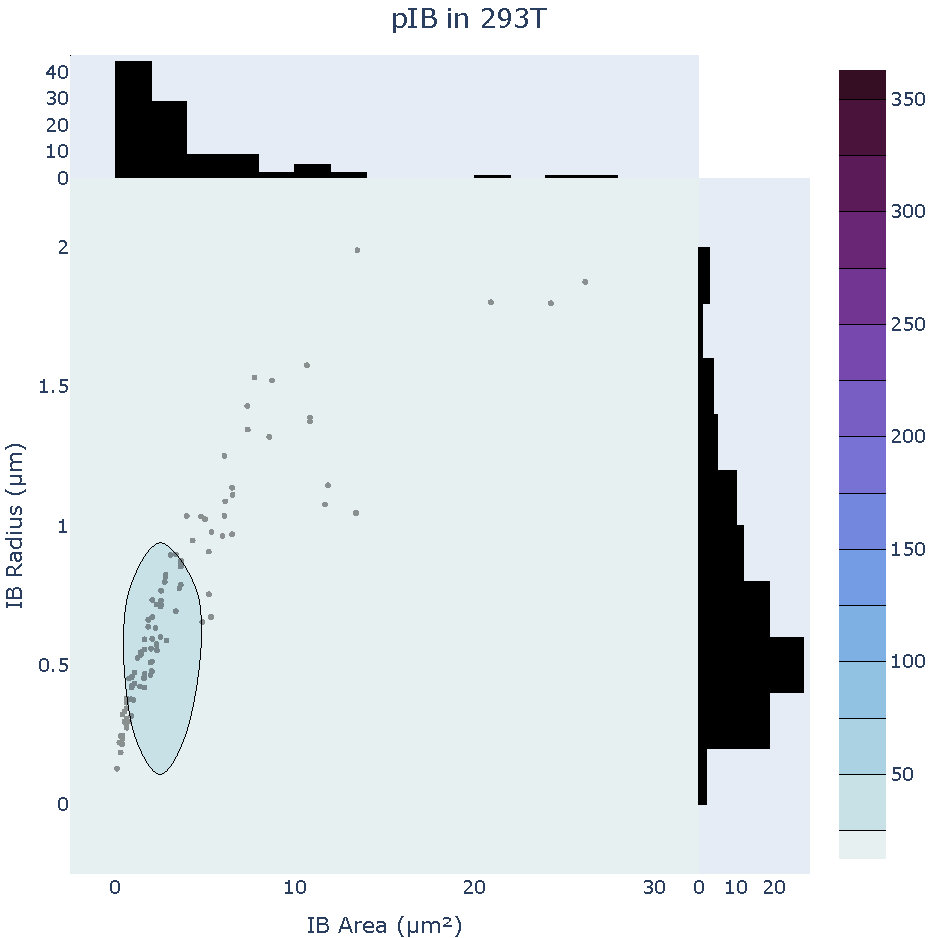
\includegraphics[width=\textwidth]{09. Chapter 4/Figs/01. pIB/01. pIB characterisation/01. heatmap_pib-293t.pdf} 
    \end{subfigure}
    \hfill
    \begin{subfigure}{0.495\textwidth}
        \caption{}
        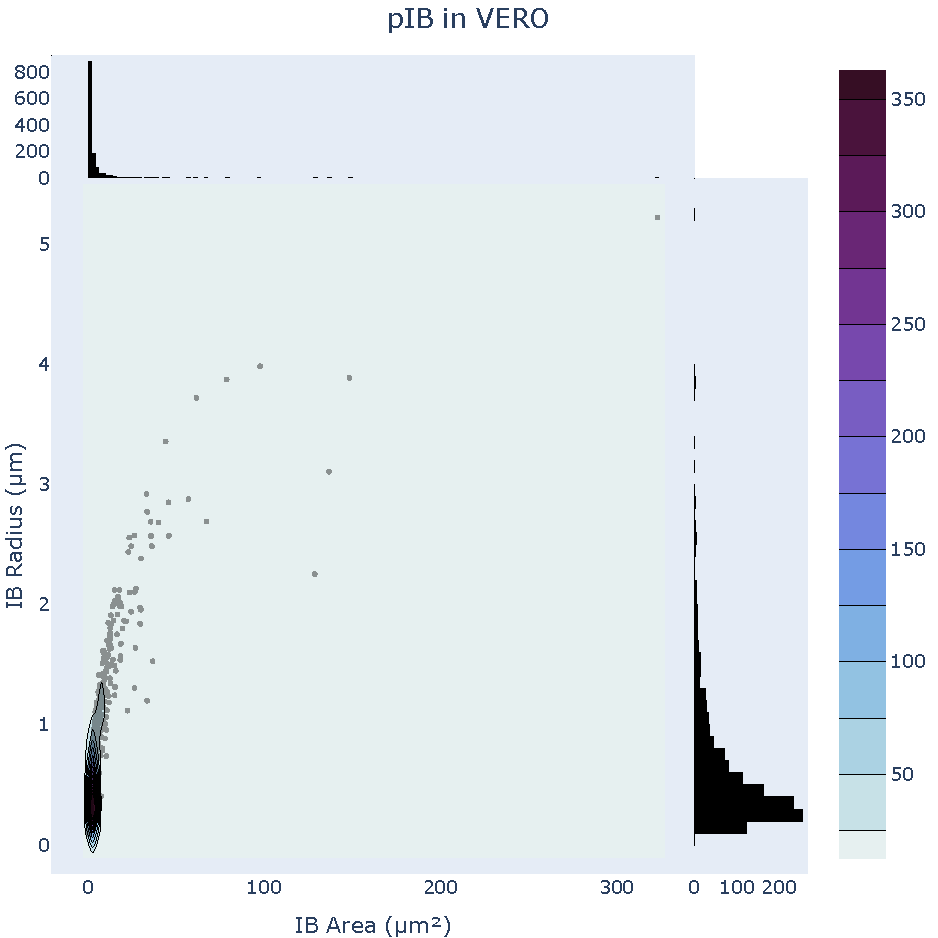
\includegraphics[width=\textwidth]{09. Chapter 4/Figs/01. pIB/01. pIB characterisation/02. heatmap_pib-vero.pdf}
    \end{subfigure}
    \caption[Size Characterisation of Pseudo Inclusion Bodies Across Different Cell Lines.]{\textbf{Size Characterisation of Pseudo Inclusion Bodies Across Different Cell Lines.} This figure presents the relationship between the measured area (\(\mu \mbox{m}^2\)) and diameter (\(\mu \mbox{m}\)) of individual pseudo inclusion bodies (pIBs) as observed within the scope of this study. Additionally, the figure includes distinct population distributions depicted alongside the plots, representing (a) 103 observations from the 293T cell line and (b) 1321 observations from the Vero cell line. Contour plots are incorporated to elucidate the underlying density of individual IBs within the plots.}
    \label{fig:Size Characterisation of Pseudo Inclusion Bodies Across Different Cell Lines}
\end{figure}

We systematically observed and annotated a total of 1424 pseudo inclusion bodies across HEK293T (103 observations) and Vero (1321 observations) cell lines. The relationship between their measured area and radia can be observed in Figure \ref{fig:Size Characterisation of Pseudo Inclusion Bodies Across Different Cell Lines}. pIBs observed in both cell lines broadly follow logaritmic curves, as expected based on the relationship of the observed values, although we can observe a sizable number of detected entities that show larger measured area compared to predicted radius. This indicates elongated ellipsioid shape. The pIBs detected in 293T cell line mainly exhibited the radia of 0.5 \(\mu \mbox{m}\), with the majority of the detected pIBs having their radia between 0.25 \(\mu \mbox{m}\) and 1 \(\mu \mbox{m}\). With regards to their associated measured area, most of the pIBs were between 0.5 \(\mu \mbox{m}^2\) and 4 \(\mu \mbox{m}^2\). In the Vero cell line we can observe a higher spread of data as we have observed pIB measuring >5 \(\mu \mbox{m}\) in radius and >300 \(\mu \mbox{m}^2\), however, majoprity of the detrected entities confronted to radia between 0.1 \(\mu \mbox{m}\) and 0.7 \(\mu \mbox{m}\), with the measured 2D area betweeen 0.1 \(\mu \mbox{m}^2\) and 4 \(\mu \mbox{m}^2\).

\begin{figure}
    \centering
    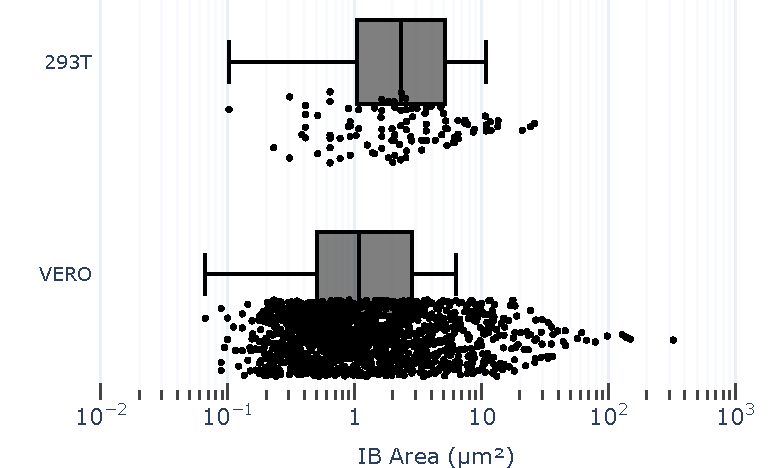
\includegraphics[width=0.75\linewidth]{09. Chapter 4/Figs/01. pIB/01. pIB characterisation/03. box-pib.pdf}
    \caption[The Distributions of pIB Areas Observed Per Cell Line.]{\textbf{The Distributions of pIB Areas Observed Per Cell Line.} The distribution of RSV pseudo inclusion body areas (\(\mu \mbox{m}^2\)), detected in this study are shown. A total of 103 observations were made in the 293T cell line, and 1321 observations in the Vero cell line.}
    \label{fig:The Distributions of pIB Areas Observed Per Cell Line}
\end{figure}

A more detailed view focusong solely on the distribution of measured areas per cell line can be observed in Figure \ref{fig:The Distributions of pIB Areas Observed Per Cell Line}. We can see that pIBs detected in Vero cell line encompas larger range in terms of the minimal and maximal measured area copared to the 293T cell line, however, the median value in the latter was higher. In more detal, in 293T cell line we have measured pIB areas ranging from sub 0.2 \(\mu \mbox{m}^2\) to supra 20 \(\mu \mbox{m}^2\), with the median value of 2.2 \(\mu \mbox{m}^2\), while in Vero cell line we have observed pIBs ranging from sub 0.07 \(\mu \mbox{m}^2\) to supra 300 \(\mu \mbox{m}^2\), with the median value of 1 \(\mu \mbox{m}^2\). Both median values are considerably smaller to what was observed in cell lines during infection (Section \ref{subsec:IFIT Subcellular Localisation During Interferon Induction and RSV Infection}, Figure \ref{fig:The Distributions of IB Areas Observed Per Cell Line}), which is in line to what was reported in literature where pIBs observed 24 hours post-transfection were considerably smaller than conventional IBs observed in infected cells after equivalent passage of time cite{Jobe2021BovineResponses}.

\begin{figure}
    \begin{subfigure}{0.495\textwidth}
        \caption{}
        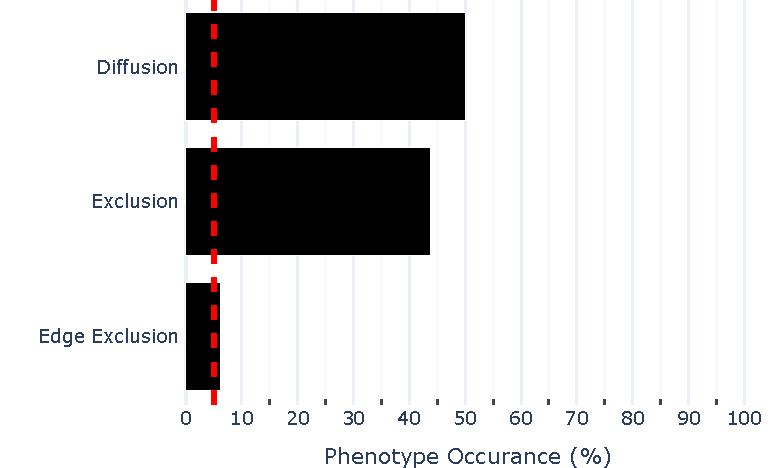
\includegraphics[width=1\linewidth]{09. Chapter 4/Figs/01. pIB/02. IFIT1/01. bar_i1_293t.pdf} 
    \end{subfigure}
    \begin{subfigure}{0.495\textwidth}
        \caption{}
        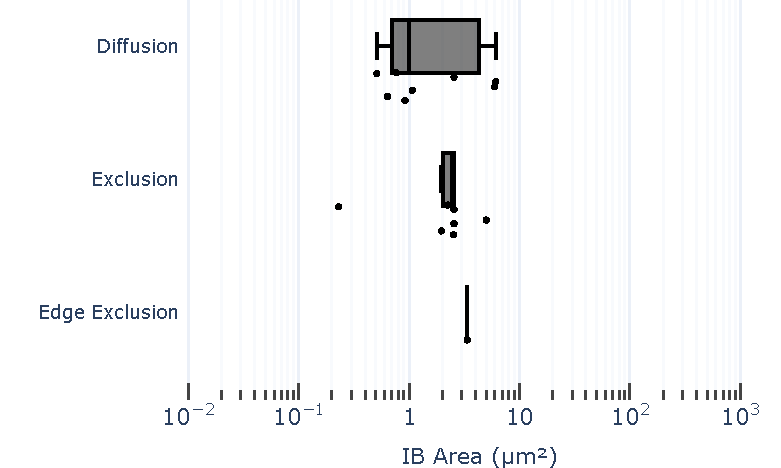
\includegraphics[width=1\linewidth]{09. Chapter 4/Figs/01. pIB/02. IFIT1/02. box_i1_293t.pdf}
    \end{subfigure}
    \caption[Phenotypic Interactions of Human IFIT1 with Human pIBs in the 293T Cell Line.]{\textbf{Phenotypic Interactions of Human IFIT1 with Human pIBs in the 293T Cell Line.} 293T cells were transfected with hRSV N and P containing plasmids using TransIT-X2 and were fixed after 24 hours. Cells were labeled with anti-RSV N and anti-IFIT1 antibodies and imaged on confocal microscope. Panel (a) shows percentual proportions of observed phenotypes between hRSV pseudo inclusion bodies and human IFIT1 (16 observations), with the red dotted line denoting the 5\% threshold, marking phenotypes considered relevant above this limit. Panel (b) shows the IB area in \(\mu \mbox{m}^2\) per observed relevant phenotype.}
    \label{fig:Phenotypic Interactions of Human IFIT1 with Human pIBs in the 293T Cell Line}
\end{figure}

\begin{figure}
    \centering
    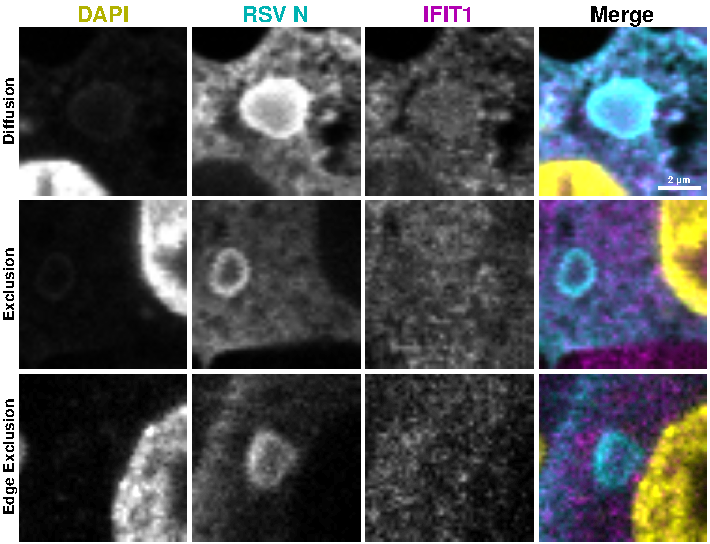
\includegraphics[width=1\linewidth]{09. Chapter 4/Figs/01. pIB/02. IFIT1/03. i1-293t-hnhp.pdf}
    \caption[Representative Images of Phenotypic Interactions of Human IFIT1 with Human pIBs in the 293T Cell Line.]{\textbf{Representative Images of Phenotypic Interactions of Human IFIT1 with Human pIBs in the 293T Cell Line.} 293T cells were transfected with hRSV N and P containing plasmids using TransIT-X2 and were fixed after 24 hours. Cellular nuclei were stained with DAPI (yellow), and cells were double-labeled with anti-RSV N (cyan) and anti-IFIT1 (magenta) antibodies. This figure showcases representative examples of relevant phenotypes in the interaction between human IFIT1 and hRSV pseudo inclusion bodies. These phenotypes are presented in descending order based on their percentage proportions. The scale bar indicates 2 \(\mu \mbox{m}\).}
    \label{fig:Representative Images of Phenotypic Interactions of Human IFIT1 with Human pIBs in the 293T Cell Line}
\end{figure}


We obtained 16 observations of endogenous human IFIT1 and its interaction with hRSV pIBs in 293T cell line. The observed phenotype frequencies, along with the measured pIB sizes can be vewed n Figure \ref{fig:Phenotypic Interactions of Human IFIT1 with Human pIBs in the 293T Cell Line}, with the representative iimagese of these phenotypes shown in Figure \ref{fig:Representative Images of Phenotypic Interactions of Human IFIT1 with Human pIBs in the 293T Cell Line}. A half of the observations displayed diffusion phenotype. This was predominantly observed in smaller pIBs with a typical size of 1 \(\mu \mbox{m}^2\) and ranging from 0.5 \(\mu \mbox{m}^2\) to 6 \(\mu \mbox{m}^2\) in size. The second most prevalent phenotype was exclusion, which occured in 44\% of cases. The pIBs associatred with this phenotype closely clustered at around 2.5 \(\mu \mbox{m}^2\), whith two exceptions i.e. one very small pIB (0.22 \(\mu \mbox{m}^2\)) and one ralitaively large pIB (5 \(\mu \mbox{m}^2\)). Lastly, we have observed one pIB with a measured area of 3.3 \(\mu \mbox{m}^2\) which exhibited size exclusion phenotype. Overall these data suggest human IFIT1 not associating with human RSV pIB structures, although this is based on a very limited set of observations.

\begin{figure}
    \begin{subfigure}{0.495\textwidth}
        \caption{}
        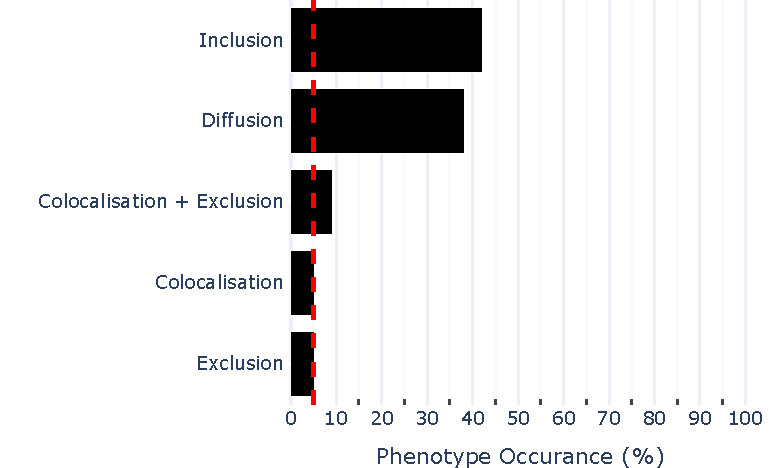
\includegraphics[width=1\linewidth]{09. Chapter 4/Figs/01. pIB/02. IFIT1/04. bar_i1_vero_hnhp.pdf} 
    \end{subfigure}
    \begin{subfigure}{0.495\textwidth}
        \caption{}
        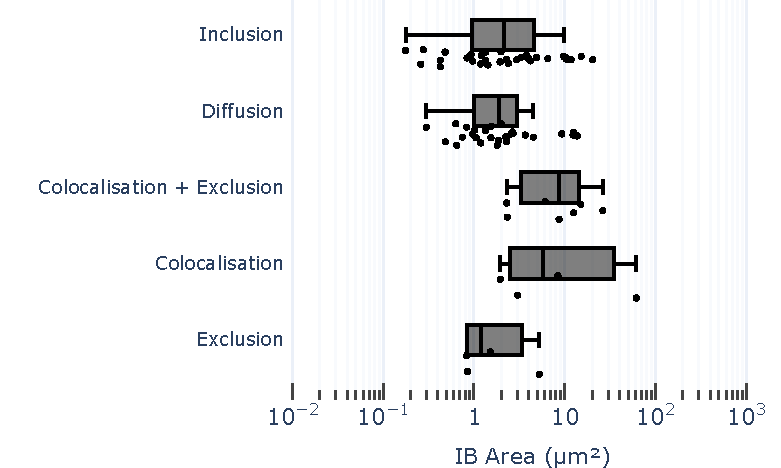
\includegraphics[width=1\linewidth]{09. Chapter 4/Figs/01. pIB/02. IFIT1/05. box_i1_vero_hnhp.pdf}
    \end{subfigure}
    \caption[Interaction Phenotypes of Monkey IFIT1 with Human pIBs in the Vero Cell Line.]{\textbf{Interaction Phenotypes of Monkey IFIT1 with Human pIBs in the Vero Cell Line.} Vero cells were transfected with hRSV N and P containing plasmids using TransIT-X2 and were fixed after 24 hours. Cells were labeled with anti-RSV N and anti-IFIT1 antibodies and imaged on confocal microscope. Panel (a) shows percentual proportions of observed phenotypes between hRSV pseudo inclusion bodies and monkey IFIT1 (76 observations), with the red dotted line denoting the 5\% threshold, marking phenotypes considered relevant above this limit. Panel (b) shows the IB area in \(\mu \mbox{m}^2\) per observed relevant phenotype.}
    \label{fig:Interaction Phenotypes of Monkey IFIT1 with Human pIBs in the VERO Cell Line}
\end{figure}

\begin{figure}
    \centering
    \includegraphics[width=1\linewidth]{09. Chapter 4/Figs/01. pIB/02. IFIT1/06. i1-vero-hnhp.pdf}
    \caption[Representative Images of Interaction Phenotypes of Monkey IFIT1 with Human pIBs in the Vero Cell Line.]{\textbf{Representative Images of Interaction Phenotypes of Monkey IFIT1 with Human pIBs in the Vero Cell Line.} Vero cells were transfected with hRSV N and P containing plasmids using TransIT-X2 and were fixed after 24 hours. Cellular nuclei were stained with DAPI (yellow), and cells were double-labeled with anti-RSV N (cyan) and anti-IFIT1 (magenta) antibodies. This figure showcases representative examples of relevant phenotypes in the interaction between monkey IFIT1 and hRSV pseudo inclusion bodies. These phenotypes are presented in descending order based on their percentage proportions. The scale bar indicates 2 \(\mu \mbox{m}\).}
    \label{fig:Representative Images of Interaction Phenotypes of Monkey IFIT1 with Human pIBs in the VERO Cell Line}
\end{figure}

Next we have evaluated endogenous monkey IFIT1 interactions with pIBs created by transfection of hRSV N and P proteins in Vero cell line. The frequencies of occurances of the interaction phenotypes based on 76 observations, along with the measured pIB areas per phenotype are shown in Figure \ref{fig:Interaction Phenotypes of Monkey IFIT1 with Human pIBs in the VERO Cell Line}. The representative images of these phenotypes are shown in Figure \ref{fig:Representative Images of Interaction Phenotypes of Monkey IFIT1 with Human pIBs in the VERO Cell Line}. 43\% of the observations show monkey IFIT1 forming intra pIB inclusion. This was followed by a diffusion phenotype, which occured in 38\% of observations. Further, 8\% of the observations showed monkey IFIT1 to be colocalisiong with the edge of the pIB structure while beiing excluded from the main pIB structure. Lastly, colocalisation and exclusion phenotypes both individually occured in 5\% of cases each. With regards to the size profile of hRSV pIBs associated with these phenotypes, inclusion was observed in a wide range of pIB sizes, ranging from sub 0.2 \(\mu \mbox{m}^2\) to supra 20 \(\mu \mbox{m}^2\) with a median size of 2 \(\mu \mbox{m}^2\). The diffusion phenotype was observed in pIBs with a smilar range of measured areas, with an identical median value of 2 \(\mu \mbox{m}^2\). These two phenotypes differ in the distribution of their values. While the pIB sizes of inclusion phenotype-associated pIBs were evenly distributed between its minimal and maximal values, diffusion-associated pIBs clustered at around 2 \(\mu \mbox{m}^2\). The colocalisation associated with pIB exclusion phenotype occured in larger pIBs with the typical area of 9 \(\mu \mbox{m}^2\) and was not observed in pIBs which were smaller than 2 \(\mu \mbox{m}^2\). The colocalisation-phenotype associated hRSV pIBs as well were of larger size, with the median value of 6 \(\mu \mbox{m}^2\), and minimal value of 2 \(\mu \mbox{m}^2\). Lastly the exclusion phenotype was was observed to be associated with 4 pIBs which had median 2D area of 1.1 \(\mu \mbox{m}^2\). Overall, although in this simplified model, the size of the pIB should not directly mean a difference in the underlying pIB complexity. Regardelss we observe size-dependent phenotype association. In smaller, sub 1 \(\mu \mbox{m}^2\) pIBs we only observed inclusiohn and diffusiion phenotyeps, which were equally prevelant in these. Larger pIBs had inclusion, diffusion and colocalisation associated with exclusion associated with them.

\begin{figure}
    \begin{subfigure}{0.495\textwidth}
        \caption{}
        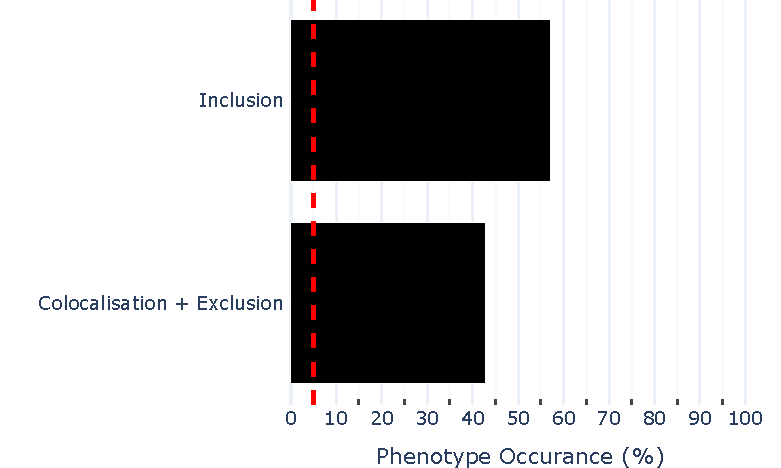
\includegraphics[width=1\linewidth]{09. Chapter 4/Figs/01. pIB/02. IFIT1/07. bar_i1_vero_bnbp.pdf}  
    \end{subfigure}
    \begin{subfigure}{0.495\textwidth}
        \caption{}
        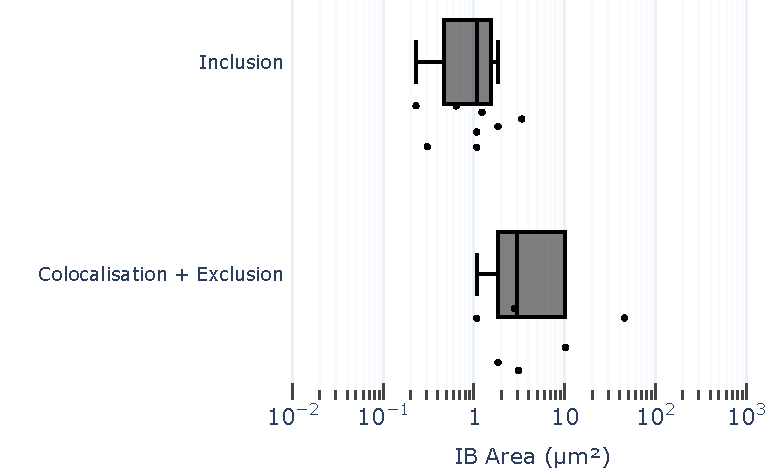
\includegraphics[width=1\linewidth]{09. Chapter 4/Figs/01. pIB/02. IFIT1/08. box_i1_vero_bnbp.pdf}
    \end{subfigure}
    \caption[Interaction Phenotypes of Monkey IFIT1 with Bovine pIBs in the Vero Cell Line.]{\textbf{Interaction Phenotypes of Monkey IFIT1 with Bovine pIBs in the Vero Cell Line.} Vero cells were transfected with bRSV N and P containing plasmids using TransIT-X2 and were fixed after 24 hours. Cells were labeled with anti-RSV N and anti-IFIT1 antibodies and imaged on confocal microscope. Panel (a) shows percentual proportions of observed phenotypes between bRSV pseudo inclusion bodies and monkey IFIT1 (14 observations), with the red dotted line denoting the 5\% threshold, marking phenotypes considered relevant above this limit. Panel (b) shows the IB area in \(\mu \mbox{m}^2\) per observed relevant phenotype.}
    \label{fig:Interaction Phenotypes of Monkey IFIT1 with Bovine pIBs in the VERO Cell Line}
\end{figure}

\begin{figure}
    \centering
    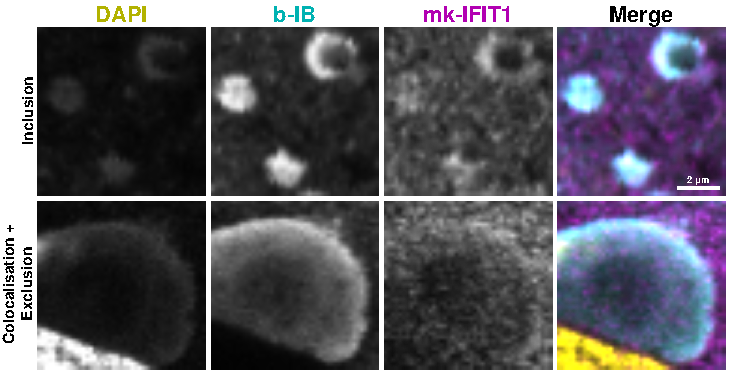
\includegraphics[width=1\linewidth]{09. Chapter 4/Figs/01. pIB/02. IFIT1/09. i1-vero-bnbp.pdf}
    \caption[Representative Images of Interaction Phenotypes of Monkey IFIT1 with Bovine pIBs in the Vero Cell Line.]{\textbf{Representative Images of Interaction Phenotypes of Monkey IFIT1 with Bovine pIBs in the Vero Cell Line.} Vero cells were transfected with bRSV N and P containing plasmids using TransIT-X2 and were fixed after 24 hours. Cellular nuclei were stained with DAPI (yellow), and cells were double-labeled with anti-RSV N (cyan) and anti-IFIT1 (magenta) antibodies. This figure showcases representative examples of relevant phenotypes in the interaction between monkey IFIT1 and bRSV pseudo inclusion bodies. These phenotypes are presented in descending order based on their percentage proportions. The scale bar indicates 2 \(\mu \mbox{m}\).}
    \label{fig:Representative Images of Interaction Phenotypes of Monkey IFIT1 with Bovine pIBs in the VERO Cell Line}
\end{figure}

Lastly we have observed monkey IFIT1 interaction,detected by human IFIT1 antibody, with bovine RSV pIBs, using the transfection of bRSV N and P containing plasmids. These plasmids consistently yielded lower transfection efficiencies and thus posed difficulties in obtaining a large amount of observations. Due to this we have failed to generate enough samples to investigate endogenous monkey IFTIs other than IFIT1 and IFIT2using the A antibody (with the respective results shown and discussed in Section \ref{subsec:Dissecting the Differential IFIT2 Antibody Staining}). Regardless, the frequencies of occurances of the interaction phenotypes based on 14 observations, along with the measured pIB areas per phenotype are shown in Figure \ref{fig:Interaction Phenotypes of Monkey IFIT1 with Bovine pIBs in the VERO Cell Line}. The representative images of these phenotypes are shown in Figure \ref{fig:Representative Images of Interaction Phenotypes of Monkey IFIT1 with Bovine pIBs in the VERO Cell Line}. We can observe results reminiscent of what was observed with IFIT2, detected by IFIT2(A) antibody during RSV infectrion. That is we observe only two phenotypes: inclusion within the pIB structures, which occurs at 56\% frequency and colocalisation associated with pIB exclusion, which occurs at 44\% frequency. The former occurs predominantly in smaller pIBs, with the median size of 1 \(\mu \mbox{m}^2\) and not bigger than 4 \(\mu \mbox{m}^2\). On the other hand, the colocalisation phenotype associated with exclusion occurs in pIBs with a typical size of 3 \(\mu \mbox{m}^2\). There is an overlap between the pIB sizes of the two phenotypes, although sub 1 \(\mu \mbox{m}^2\) pIBs are always associated with inclusion while supra 10 \(\mu \mbox{m}^2\) are always associated with colocalisation cojoined with exclusion.

Taking all of the IFIT1-pIB interaction results together it seems like there is a differential propensity for pIB interaction between endogenous human and monkey IFIT1. Saying that, data obtained from HEK293T cell line is limited in quantity and displays a size bias towards pIBs that are less than 6 \(\mu \mbox{m}^2\) in size. This does not correspond to the true diversity of pIB sizes observed in this study as the aggregate 293T suggest there is a sizable population of supra 6 \(\mu \mbox{m}^2\) pIBs that was detected in this study (Figure \ref{fig:The Distributions of pIB Areas Observed Per Cell Line}). In the Vero cell line transfected with hRSV N and P ORF-containing plasmids, we have observed phenotypes that imply direct interaction (colocalisation and colocalisation asssociated with exclusion) specificaly in larger pIBs. This implies that the limited sample size and diversity in 293T observed hRSV pIBs is not sufficient to provide true picture of IFIT1/pIB interaction. On the other hand, it can be also implicative of hIFIT1 not being recruited to the pIBs. Within the Vero cell line we also ofbserved differential results which dependent on the species of the virus. While we have only observed direct interaction phenotypes of inclusion formation and pIB edge colocalsiation with intra-pIB exclusion with the bRSV pIBs, we observed a more diverse interaction range in Vero cells with hRSV pIBs present in them. These phenotypes, however, all, with the exeption of exclusion phenotype (which occured only in 5\% of observations), implied IFIT1 having access to the pIB structure. It is intrueegin to see the differences between humand and bovine RSV pIB and their interaction with monkey IFIT1. This could suggest that the bovine pIB possibly lack mechanism that would prevent them from being targeted by the moneky IFIT1. Saying that, the bovine RSV pIB dataset lacks inthe depth with regards to the amount of observations, and thus the differences could also be atributed to low frequency of diffusion or exclusion phenotypes. In that case the results from Vero cell lines with either human or bovine RSV pIBs present would be almost identical.

\begin{figure}
    \begin{subfigure}{0.495\textwidth}
        \caption{}
        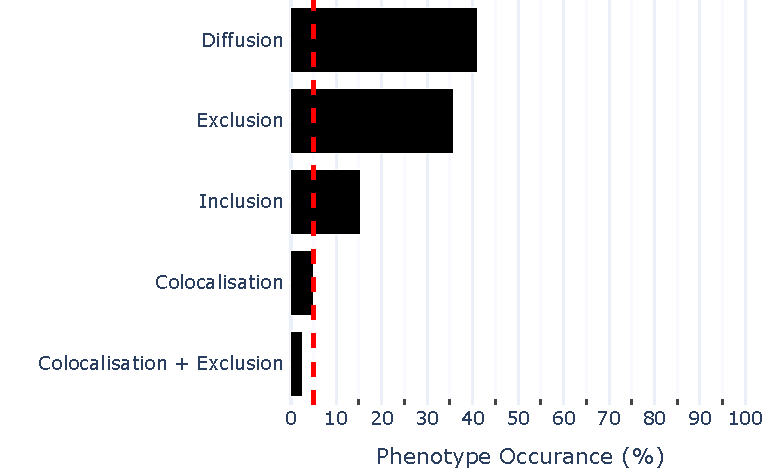
\includegraphics[width=1\linewidth]{09. Chapter 4/Figs/01. pIB/04. IFIT3/01. bar_i3_vero.pdf} 
    \end{subfigure}
    \begin{subfigure}{0.495\textwidth}
        \caption{}
        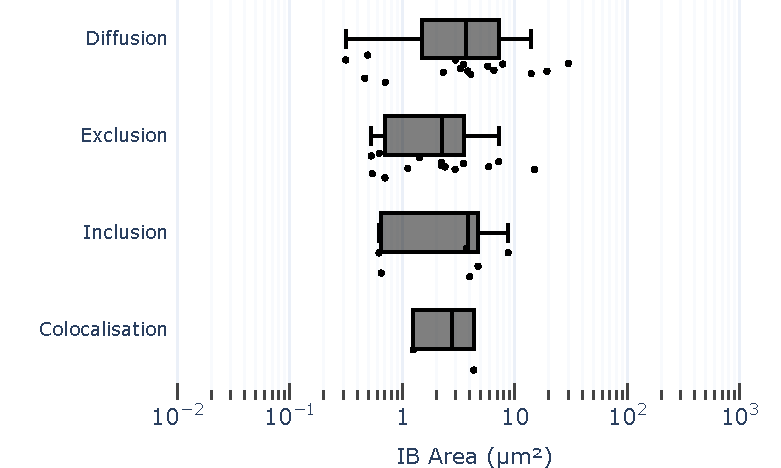
\includegraphics[width=1\linewidth]{09. Chapter 4/Figs/01. pIB/04. IFIT3/02. box_i3_vero.pdf}
    \end{subfigure}
    \caption[Interaction Phenotypes of Monkey IFIT3 with Human pIBs in the Vero Cell Line.]{\textbf{Interaction Phenotypes of Monkey IFIT3 with Human pIBs in the Vero Cell Line.} Vero cells were transfected with hRSV N and P containing plasmids using TransIT-X2 and were fixed after 24 hours. Cells were labeled with anti-RSV N and anti-IFIT3 antibodies and imaged on confocal microscope. Panel (a) shows percentual proportions of observed phenotypes between hRSV pseudo inclusion bodies and monkey IFIT3 (39 observations), with the red dotted line denoting the 5\% threshold, marking phenotypes considered relevant above this limit. Panel (b) shows the IB area in \(\mu \mbox{m}^2\) per observed relevant phenotype.}
    \label{fig:Interaction Phenotypes of Monkey IFIT3 with Human pIBs in the VERO Cell Line}
\end{figure}

\begin{figure}
    \centering
    \includegraphics[width=1\linewidth]{09. Chapter 4/Figs/01. pIB/04. IFIT3/03. i3-vero-hnhp.pdf}
    \caption[Representative Images of Interaction Phenotypes of Monkey IFIT3 with Human pIBs in the Vero Cell Line.]{\textbf{Representative Images of Interaction Phenotypes of Monkey IFIT3 with Human pIBs in the Vero Cell Line.} Vero cells were transfected with hRSV N and P containing plasmids using TransIT-X2 and were fixed after 24 hours. Cellular nuclei were stained with DAPI (yellow), and cells were double-labeled with anti-RSV N (cyan) and anti-IFIT3 (magenta) antibodies. This figure showcases representative examples of relevant phenotypes in the interaction between monkey IFIT3 and hRSV pseudo inclusion bodies. These phenotypes are presented in descending order based on their percentage proportions. The scale bar indicates 2 \(\mu \mbox{m}\).}
    \label{fig:Representative Images of Interaction Phenotypes of Monkey IFIT3 with Human pIBs in the VERO Cell Line}
\end{figure}

Next we investigated IFIT3 interaction with RSV pseudo incluson bodies. As mentioned above we failed to generate samples concisting either of HEK293T cells transfected with hRSV N and P, or Vero cells transfected with bRSV N and P, which would be also stained for IFIT3. Hence we only present the monkey IFIT3 interaction analysis with hRSV pIBs. The frequencies of observed phenotypes within the 39 observations along with the measured pIB sizes per phenotype which occur with more than 5\% frequency are shown in Figure \ref{fig:Interaction Phenotypes of Monkey IFIT3 with Human pIBs in the VERO Cell Line}. The representative images of phenotypes which occur with at  least 5\% frequency are shown in Figure \ref{fig:Representative Images of Interaction Phenotypes of Monkey IFIT3 with Human pIBs in the VERO Cell Line}. The most prevalent phenotype is diffusn throught the pIB structure, which occured at 41\% of observation. This was closely followed by an exclusion phenotype, which occured at 36\% of observations. We have observed monkey IFIT3 to be forming intra pIB inclusion in 15\% of the cxases. Laslty, 5\% of observations showed colocalisation phenotype, while 3\% of all observations shopwed colocalisation associated with exclusion. With regards of the size profile of the IBs associated with the different phenotyeps which displayed at least 5\% frequency, their median values seem to be quite similar, however they encompass a progressivelymore narrow range of values as the occurance frequency decreases. In more detail the diffusion phenotype median pIB size was 4 \(\mu \mbox{m}^2\) and it encompasses values from 0.3 \(\mu \mbox{m}^2\) to 30 \(\mu \mbox{m}^2\). The exclusion phenotype-associated median area value was 2 \(\mu \mbox{m}^2\), while the range of sizes of the detected pIBs encompassed sub 0.6 \(\mu \mbox{m}^2\) to supra 10 \(\mu \mbox{m}^2\). The size values of inclusion-associated pIBs clustered at around 3 \(\mu \mbox{m}^2\) and ranged from two observations at 6 \(\mu \mbox{m}^2\) to one observation at 9 \(\mu \mbox{m}^2\). Lastly, the pIBs associated with the colocalisation phenotype were of 1.3 \(\mu \mbox{m}^2\) and 4.3 \(\mu \mbox{m}^2\). It seems like predominantly in most cases monkey IFIT3 is not directly seen interacting with the hRSV pIB structures, however in a quater of the cases it seems to be either forming inclusions or being associated with the edge of the pIB strucutre. This data seems to confirm our earlier investigation where IFIT3 exhibited predominantly exclusion and diffusion phenotypes during RSV infection.

\begin{figure}
    \begin{subfigure}{0.495\textwidth}
        \caption{}
        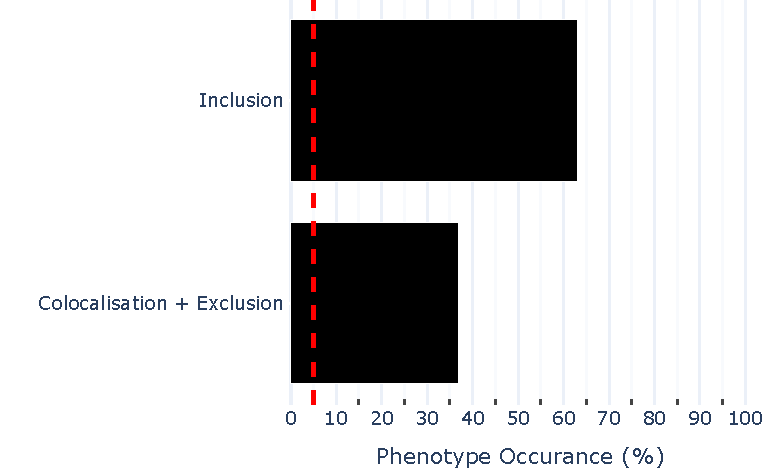
\includegraphics[width=1\linewidth]{09. Chapter 4/Figs/01. pIB/05. IFIT5/01. bar_i5_vero.pdf} 
    \end{subfigure}
    \begin{subfigure}{0.495\textwidth}
        \caption{}
        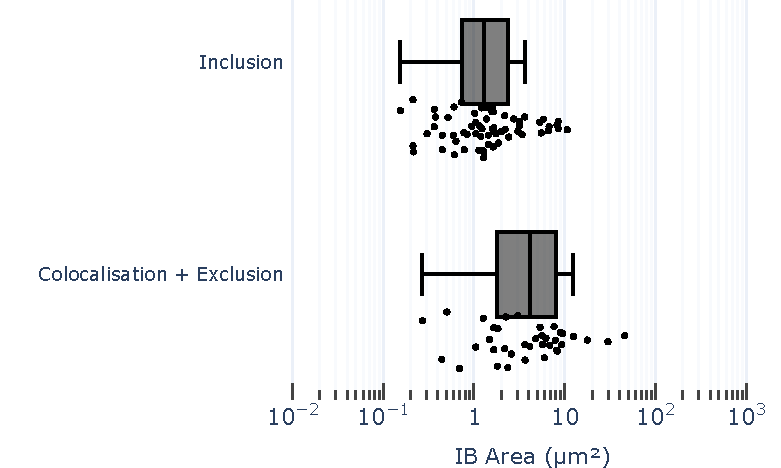
\includegraphics[width=1\linewidth]{09. Chapter 4/Figs/01. pIB/05. IFIT5/02. box_i5_vero.pdf}
    \end{subfigure}
    \caption[Interaction Phenotypes of Monkey IFIT5 with Human pIBs in the Vero Cell Line.]{\textbf{Interaction Phenotypes of Monkey IFIT5 with Human pIBs in the Vero Cell Line.} Vero cells were transfected with hRSV N and P containing plasmids using TransIT-X2 and were fixed after 24 hours. Cells were labeled with anti-RSV N and anti-IFIT5 antibodies and imaged on confocal microscope. Panel (a) shows percentual proportions of observed phenotypes between hRSV pseudo inclusion bodies and monkey IFIT5 (100 observations), with the red dotted line denoting the 5\% threshold, marking phenotypes considered relevant above this limit. Panel (b) shows the IB area in \(\mu \mbox{m}^2\) per observed relevant phenotype.}
    \label{fig:Interaction Phenotypes of Monkey IFIT5 with Human pIBs in the VERO Cell Line}
\end{figure}

\begin{figure}
    \centering
    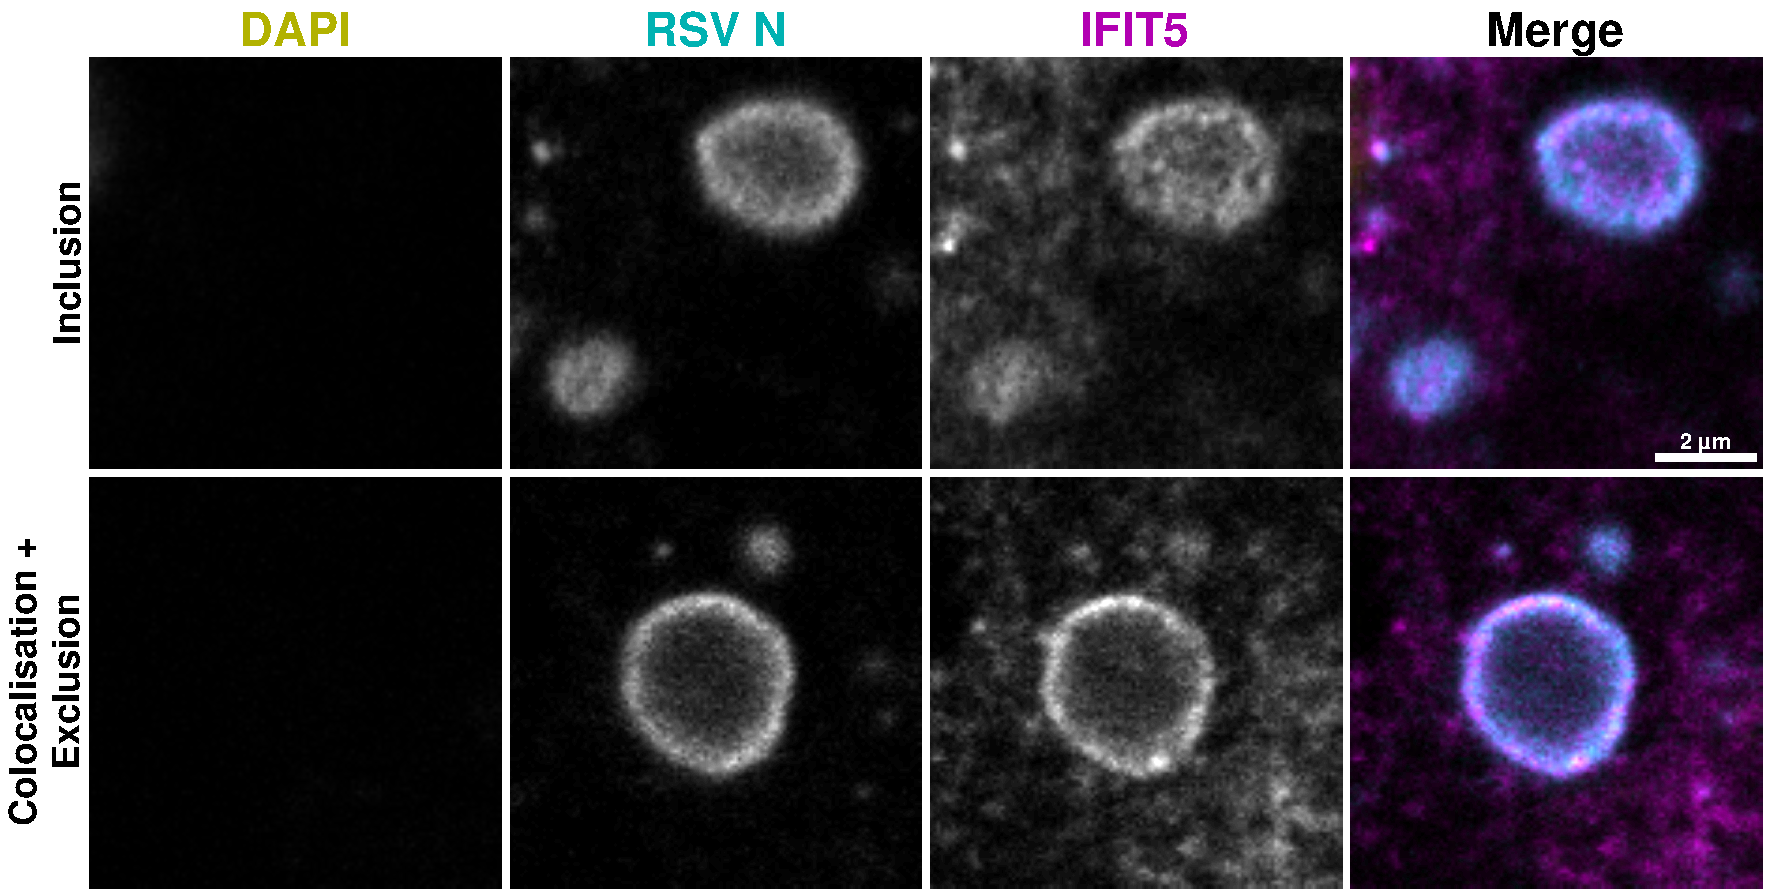
\includegraphics[width=1\linewidth]{09. Chapter 4/Figs/01. pIB/05. IFIT5/03. i5-vero-hnhp.pdf}
    \caption[Representative Images of Interaction Phenotypes of Monkey IFIT5 with Human pIBs in the Vero Cell Line.]{\textbf{Representative Images of Interaction Phenotypes of Monkey IFIT5 with Human pIBs in the Vero Cell Line.} Vero cells were transfected with hRSV N and P containing plasmids using TransIT-X2 and were fixed after 24 hours. Cellular nuclei were stained with DAPI (yellow), and cells were double-labeled with anti-RSV N (cyan) and anti-IFIT5 (magenta) antibodies. This figure showcases representative examples of relevant phenotypes in the interaction between monkey IFIT5 and hRSV pseudo inclusion bodies. These phenotypes are presented in descending order based on their percentage proportions. The scale bar indicates 2 \(\mu \mbox{m}\).}
    \label{fig:Representative Images of Interaction Phenotypes of Monkey IFIT5 with Human pIBs in the VERO Cell Line}
\end{figure}

Lastly we have investigated the IFIT5 interactions with the simplified system of RSV pseudo inclusion bodies. As mentioned previously we only managed to obtain data from Vero cell line transfected with hRSV N and P containing plasmids and thus we can only investigate the monkey IFIT5 interaction with the human pIBs. Figure \ref{fig:Interaction Phenotypes of Monkey IFIT5 with Human pIBs in the VERO Cell Line} shows the frequencies of occurances of the observed phenotypes alongside the measured pIB areas per observed phenotype from the 100 observations that were recorded. Figure \ref{fig:Representative Images of Interaction Phenotypes of Monkey IFIT5 with Human pIBs in the VERO Cell Line} shows the representative images of these pehnotypes. We have observed monkey IFIT5 to exert two hRSV pIB interaction phenotypes i.e. to be forming intra-pIB inclusion or to colocalise with the pIB boundry while being excluded from the pIB structure. The former occured in 62\% of observations, while the latter occured in 38\% of observations. The size of inclusion-associated hRSV pIBs ranged from 0.13 \(\mu \mbox{m}^2\) to 10 \(\mu \mbox{m}^2\), with atypiocal value of 1.2 \(\mu \mbox{m}^2\). On the other hand the size profile of pIBs associated with colocalisation acompalied by exclusion phenotype ranged from 0.23 \(\mu \mbox{m}^2\) to supra 40 with the median value of 4 \(\mu \mbox{m}^2\). There seams to be a differentiation of these pIBs based on size although there is a marked overlap of sizes where both phenotypes occur (between 0.23 and 10 \(\mu \mbox{m}^2\)). Interestingly, previously we have observed both human and bovine IFIT5 to be minimaly interacting with the RSV IBs, with the most prevalent observed phenotype being exclusion (Chapter \ref{ch:Subcellular Localisation of Endogenous IFIT Proteins in the Context of RSV Inclusion Bodies}). We have observed the inclusion phenotype only in 10\% of observations in MDBK cell line and the colocalisation associated with exclusioin phenotype in 5\% of observations in A549 cell line. This suggest that IFIT5 has a propensity to interact with the pseudo inclusion bodies but some factors that are present in RSV IBs during infection are preventing IFIT5 from accessing these structures.

Overall the investigaton of IFIT1, IFIT3, and IFIT5 localisation with regards to the simplified model of RSV inclusion bodies using ectopically expressed pseudo-inclusion bodies yielded somewhat interesting results, which can lead us to uncover the nature of thier interactions and the potential factors that are impeeding these intreactions during RSV infection. With regards to endogenous IFIT1, we have observed minimal interaction in human cells (HEK293T) with hRSV pIBs, although this could have been as a result of size bias of the observed pIBs. We base this assumption based on the observed monkey IFIT1 interactions with human RSV pIBs, where the strong interaction phenotypes (inclusion and colocalisation) correlated with increased pIB size, and especially based on the results from monkey IFIT1 interaction with bovine RSV pIBs where we solely observed phenotypes implying interaction. The monkey IFIT1 data supports the observations from Section \ref{subsec:Endogenous IFIT Interaction with RSV Inclusion Bodies}, where we have observed both human and bovine IFIT1 show strong interaction phenotypes (incluson or colocalisation) with RSV IBs during infection. However this was not the domiminant phenotype observed, which was exclusion. Clearly IFIT1 has a propensity to directly associate with the pIB, a process which seems to be disrupted during infection. Monkey IFIT3 displayed data consistent to what was observed in RSV infection data i.e. majority of the cases being either indirectly associated with pIBs (diffusion), or being excluded from the structures, while directly associating with these strucutres with small but considerable frequency. This suggest that the IFIT3-IB intreraction is directied via biophysical interactions with the pIB and IB structures. Lastly, monkey IFIT5 showed only strong interaction phenotypes with human pIBs. This is unexpected as during infection neither human nor bovine IFIT5 exhibited minimal direct or indirect interaction phenotypes, with the dominant observed phenotype being exclusion. This discrepancy could be due to the diffrential propensity of monkey IFIT5 for interaction with (p)IBs compared to human and bovine IFIT5, or it could mean that viral  or cellular factors associated with and influencing the RSV IBs during infection prevent IFIT5 from interaction with these structures. Overall while these experiments provided us with valuable data that confirmed ourprevious observations (as is the case for IFIT3, or IFIT1 interacting with human pIBs), it has also yielded data which is inconbsistent with previous observations. The other issue is that majority of the gathered data is based on monkey IFITs which are not relevant for human and bovine RSV infection \textit{in vivo}. Thus it is esential that these data is further validated and investrigated using human and bovine IFITs. To do this we aimed to analyse the interaction profiles of exogenbously expressed human and bovine IFITs in the context of human and bovine RSV infection.

\subsection{Overexpressed IFIT1, IFIT3, and IFIT5 During RSV Infection} \label{subsec:Overexpressed IFIT1, IFIT3, and IFIT5 During RSV Infection}
In order to validate the interaction results of monkey IFIT1, IFIT3, and IFIT5 with pseudo IBs and to investigate the maximal potential for intereactions between human and bovine IFIT1, IFIT3, and IFIT5 with human and bovine IBs in the context of infection, we further aimed to conduct IFIT overexpression expreiments coupled with RSV infection. We wanted to decrease the likelihood of nonspecific antibody staining by overexpressing FLAG-tagged IFIT proteins, which would be visualised using monoclonal anti-FLAG antibody. The usage of FLAG tag would allow for higher specificity and increased access for IB detection inside of the phase separated structures \cite{Munro1984Use70.}. To do this we needed a library of FLAG-tagged human and bovine IFIT proteins, cloned in plasmids which allow for effcient translation in transfected cells. We were kindly provided with human IFIT1, IFIT2, IFIT3, and IFIT5 ORF-containng plasmids, each tagged with FLAG in the C terminus by the Viral Gene Expressioin group from the Pirbright Institute. This group also provided a control GFP-FLAG pcDNA3.1 plasmid, which was used as a control for transfection efficiency and persistance. These were already present in a  pcDNA3.1 backbone, whcih was directly suitable for our downstream analyses. We were also kindly provided by bovine IFIT-containing plasmids by CVR Glasgow as a part of their bovine ISG plasmid library. There plasmids were consisting of SCRPSY backbone, which is optimasied for creating lentiviral praticles, and untagged bovine IFIT ORFs. Due to this reason we needed to clone these ORF into pcDNA3.1 plasmid backbone, while cocurently adding a C-terminal FLAG tag.

The schematics and decriptions of the pcDNA3.1 and SCRPSY plasmids are depicted in Section \ref{subsec:DNA Plasmids}, while the detailed description of cloning and subcling methodologies are shown in Section \ref{subsec:PCR for Cloning into pcDNA3.1} and Section \ref{subsec:Common Subcloning Methodologies} respectively. Briefly, we have designed forwards and reverse primers, specific for each bovine \textit{IFITs}, consisting of, among other elements, section of the ORF, FLAG tag, start or stop sequence, and the recognition sites of Acc65I and NotI restriction enzymes respectively. These were specificaly selected as their restrictioni sites are not preset within either of the bovine \textit{IFIT} sequence. These primers were used to PCR amplify and isolate the bovine \textit{IFIT} ORFs from the SCRPSY plasmids. These linear ORFs were subsequently subcloned into the pcDNA3.1 plasmid backbones.

To assay the subcellular localisation of exogenously expressed human and bovine IFIT proteins with regards to human and bovine RSV inclusion bodies, we have transfected Vero cells with 1 \(\mu\)g per well of a 24 well plate using TransIT-X2, as decribed in Section \ref{subsec:Transfecting Cells}, and infected the cells with MOI 1 RSV based on the standard methodology (described in Section \ref{subsec:Viral Infections, UV-Inactivation and Ruxolitinib Treatment}). There is an inherent difficulty in establishing cocurrent infection and transfection in the same cells, as doing one treatment usually puts the cell in a antiviral state, that prevents further treatment (infection or transfection). Due to this, we have to tried several methodologies to cause cocurrent infection and transfection. To obtain data that would be comparable with the data previously gathered from infectiion experiments (Chapter \ref{ch:Subcellular Localisation of Endogenous IFIT Proteins in the Context of RSV Inclusion Bodies}) i.e. RSV infection that is terminated 24 HPI, we have initialy tried cell transfection, that was follwed by RSV infection 24 hours post transfection. We used the GFP-FLAG control plasmid to easily assess transfection efficiency and persistance, while we have examined the cells for RSV cytophatic effect (e.g. syncytia formation) to confirm sucessful infection. While we were able to detect sucesful transfection 24 hours post transfection, after 24 hours of subvsequent infection none GFP-expression was detected. Next, we have tried simultanoues infection and transfection. This was done by initial inoculatyion of the cells with a virus preparation and incubation with this innoculum for an hour. Afterwards the inoculum was removed, the cells washed with PBS, after which the trabsfection mixture was added in the cell culture media. This however also resulted in minimal GFP expression. In both of these methodologies we have observed robust infection. Lastly we have emplyed initial RSV infection, followed by transfection 24 HPI. The cells were fixed 24 hours post transfection i.e. 48 hours post infection. This methogology yielded the best co-infection/transfection out of all methodologies tried. Saying this, it was still sub optimal as for some IFIT/RSV conbinations we have only detected 10-15 co-infection/transfection cells, although sufficient for confocal microscopy analysis.

This is to be expected as we know that overexpressed hIFIT1, hIFIT2, and hIFIT3 are antiviral against RSV and thus cells that would present ectopicaly expressded IFITs would therefore create an enviroment that would be unbsuitable for RSV life cycle. Along to this and as mantioned above, infected cells activate their innate antiviral pahtwasys and thus prevent another infection or transfection. This creates inherent bias whereby the cells which have the propensity to be coccurently infected and transfected are not representative of the general cellular population. With regards to the lenght of the infection, after 48 HPI we can expect the size of the IBs to be substantialy larger to what we observed at 24 HPI previously. It is reported in the literature that the mean 2D area of bRSV incusion bodies increased from 8.99 \(\mu \mbox{m}^2\) to 22.18 \(\mu \mbox{m}^2\) between 24 HPI and 48 HPI \cite{Jobe2021BovineResponses}. This would thus make it difficult to compare the co-infection/transfection data to the infection data from Chapter \ref{ch:Subcellular Localisation of Endogenous IFIT Proteins in the Context of RSV Inclusion Bodies}. We could however use the present data to investigate the potential influence of ectopicaly expressed IFIT proteins on the 2D IB area, which could be used to gauge the potential anti-RSV mechanism of these proteins. We experienced difficulties in obtaining co-infection/transfection data with several plasmids. These include bovine IFIT1, human IFIT3, and bovine IFIT5. These were possibly die to a variety of reasons e.g. decreased teransfection efficiency due to contaminats present in the plasmid preparation or the tranfection complexex failing to form properly. All of the data presented below is supported by z-stack measurements.

\begin{figure}
    \begin{subfigure}{0.495\textwidth}
        \caption{}
        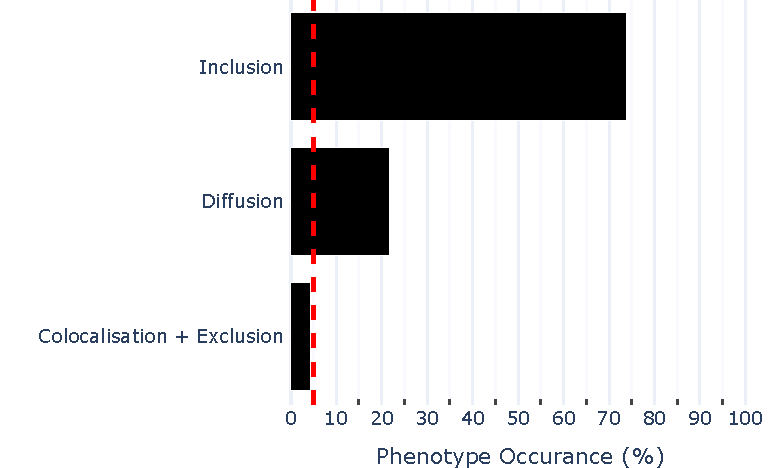
\includegraphics[width=1\linewidth]{09. Chapter 4/Figs/02. Overexpression/01. IFIT1/01. bar_i1_hrsv.pdf} 
    \end{subfigure}
    \begin{subfigure}{0.495\textwidth}
        \caption{}
        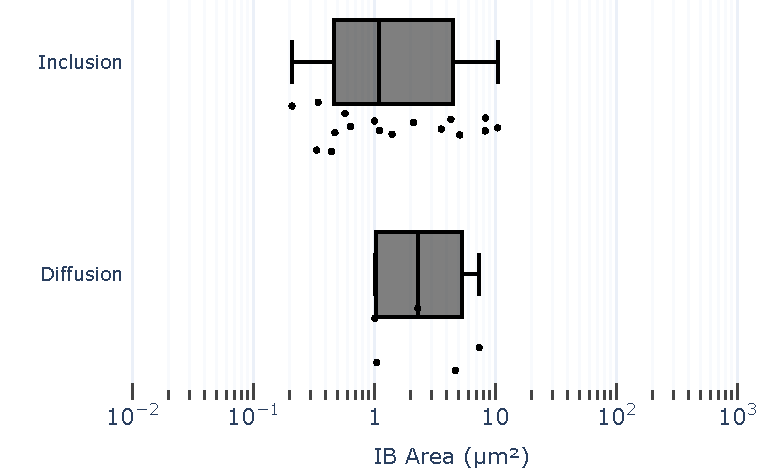
\includegraphics[width=1\linewidth]{09. Chapter 4/Figs/02. Overexpression/01. IFIT1/02. box_i1_hrsv.pdf}
    \end{subfigure}
    \caption[Observed Phenotypes of Exogenous hIFIT1 in the Context of hRSV Inclusion Bodies in Vero Cell Line.]{\textbf{Observed Phenotypes of Exogenous hIFIT1 in the Context of hRSV Inclusion Bodies in Vero Cell Line.} Vero cells were infected with human RSV at MOI 1. 24 HPI, the cells were transfected with hIFIT1-FLAG containing plasmids using TransIT-X2 and were fixed after a further 24 hours. Cells were labelled with anti-RSV N and anti-FLAG antibodies and imaged on a confocal microscope. Panel (a) shows the percentual proportions of observed phenotypes between hRSV inclusion bodies and exogenous hIFIT1 (23 observations), with the red dotted line denoting the 5\% threshold, marking phenotypes considered relevant above this limit. Panel (b) shows the IB area in \(\mu \mbox{m}^2\) per observed relevant phenotype.}
    \label{fig:Observed Phenotypes of Exogenous hIFIT1 in the Context of hRSV Inclusion Bodies in VERO Cell Line}
\end{figure}

\begin{figure}
    \centering
    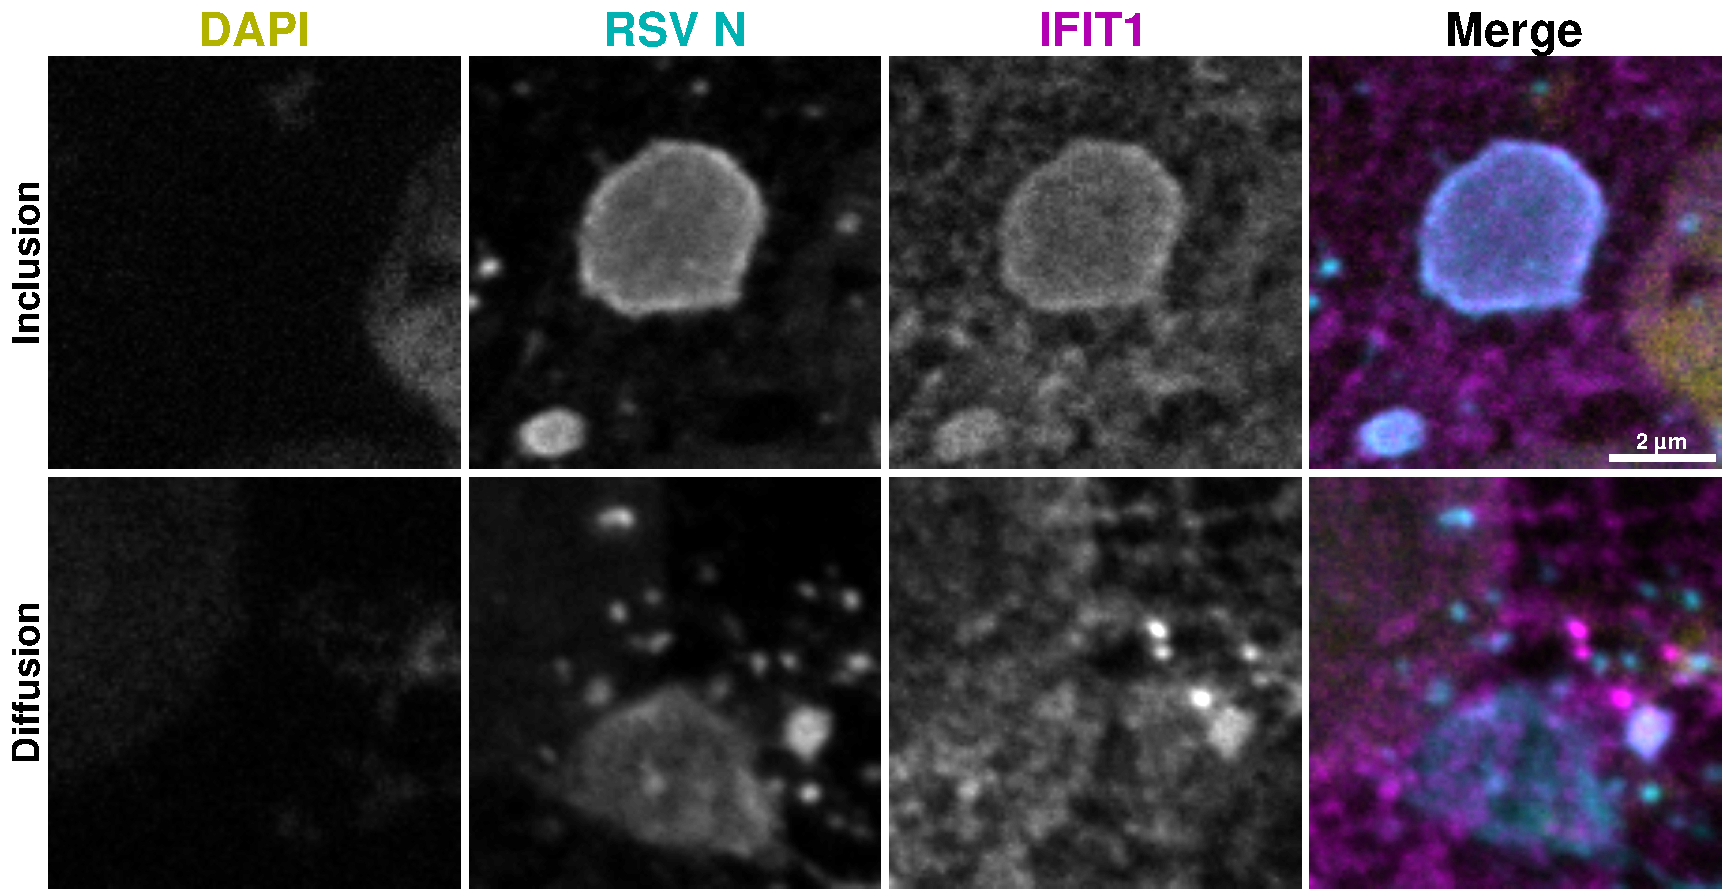
\includegraphics[width=1\linewidth]{09. Chapter 4/Figs/02. Overexpression/01. IFIT1/03. i1-hrsv.pdf}
    \caption[Representative Images of Observed Phenotypes of Exogenous hIFIT1 in the Context of hRSV Inclusion Bodies in Vero Cell Line.]{\textbf{Representative Images of Observed Phenotypes of Exogenous hIFIT1 in the Context of hRSV Inclusion Bodies in Vero Cell Line.} Vero cells were infected with human RSV at MOI 1. 24 HPI, the cells were transfected with hIFIT1-FLAG containing plasmids using TransIT-X2 and were fixed after a further 24 hours. Cellular nuclei were stained with DAPI (yellow), and cells were double-labelled with anti-RSV N (cyan) and anti-FLAG (magenta) antibodies. This figure showcases representative examples of relevant phenotypes in the interaction between exogenous hIFIT1 and hRSV inclusion bodies. These phenotypes are presented in descending order based on their percentage proportions. The scale bar indicates 2 \(\mu \mbox{m}\).}
    \label{fig:Representative Images of Observed Phenotypes of Exogenous hIFIT1 in the Context of hRSV Inclusion Bodies in VERO Cell Line}
\end{figure}

We have observed 23 instances of human IFIT1 being expressed in hRSV infected cells. The frequencies of occurances of observed phenotypes along to the measured IB sizes of phenotypes occuring with >5\% fruequency are shown in Figure \ref{fig:Observed Phenotypes of Exogenous hIFIT1 in the Context of hRSV Inclusion Bodies in VERO Cell Line}. The representative images of the latter are shown in Figure \ref{fig:Representative Images of Observed Phenotypes of Exogenous hIFIT1 in the Context of hRSV Inclusion Bodies in VERO Cell Line}. The most commonly occurng phenotype was intra-IB inclusion, which was observed in 74\% of observations. This was followed by a diffusioin phenotype (22\%), and colocalisation associated with IB exclusion (4\%). Since the latter occured in sub 5\% frequency it was exluded from the size analysis. With regards to the size of inclusion phenotype-associated IBs, they encompasses the whole size spectrum of the IBs observed in this condition (i.e. hIFIT1 and hRSV co-infection/transfection) ranging from 0.2 \(\mu \mbox{m}^2\) to 10 \(\mu \mbox{m}^2\), with the typical size of 1.1 \(\mu \mbox{m}^2\). The diffusion-associated IBs were observed to be between 1 \(\mu \mbox{m}^2\) and 7 \(\mu \mbox{m}^2\) in size, with the median value of 2.2 \(\mu \mbox{m}^2\). This shows that small sub 1 \(\mu \mbox{m}^2\) IBs specificaly present inclusion phenotyoe while the medium sized IBs dyspolay both inclusion and diffusion phenotypes. Interestiingly we have not observed IBs larger than 10 \(\mu \mbox{m}^2\), which is unusual for for IBs observed at 48 HPI. The reason could be the anti RSV action of hIFIT1.

\begin{figure}
    \begin{subfigure}{0.495\textwidth}
        \caption{}
        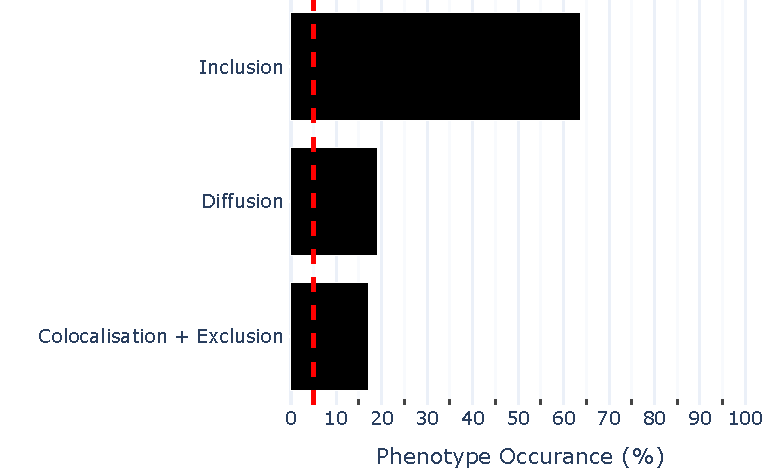
\includegraphics[width=1\linewidth]{09. Chapter 4/Figs/02. Overexpression/01. IFIT1/04. bar_i1_brsv.pdf} 
    \end{subfigure}
    \begin{subfigure}{0.495\textwidth}
        \caption{}
        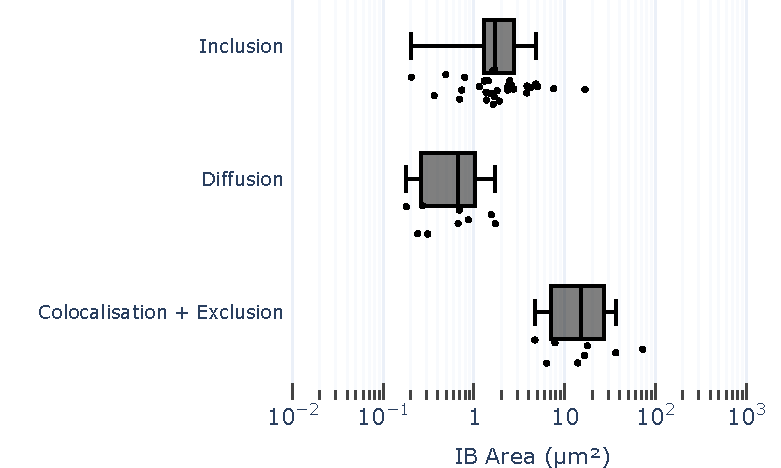
\includegraphics[width=1\linewidth]{09. Chapter 4/Figs/02. Overexpression/01. IFIT1/05. box_i1_brsv.pdf}
    \end{subfigure}
    \caption[Observed Phenotypes of Exogenous hIFIT1 in the Context of bRSV Inclusion Bodies in Vero Cell Line.]{\textbf{Observed Phenotypes of Exogenous hIFIT1 in the Context of bRSV Inclusion Bodies in Vero Cell Line.} Vero cells were infected with bovine RSV at MOI 1. 24 HPI, the cells were transfected with hIFIT1-FLAG containing plasmids using TransIT-X2 and were fixed after further 24 hours. Cells were labeled with anti-RSV N and anti-FLAG antibodies and imaged on confocal microscope. Panel (a) shows percentual proportions of observed phenotypes between bRSV inclusion bodies and exogenous hIFIT1 (47 observations), with the red dotted line denoting the 5\% threshold, marking phenotypes considered relevant above this limit. Panel (b) shows the IB area in \(\mu \mbox{m}^2\) per observed relevant phenotype.}
    \label{fig:Observed Phenotypes of Exogenous hIFIT1 in the Context of bRSV Inclusion Bodies in VERO Cell Line}
\end{figure}

\begin{figure}
    \centering
    \includegraphics[width=1\linewidth]{09. Chapter 4/Figs/02. Overexpression/01. IFIT1/06. i1-brsv.pdf}
    \caption[Representative Images of Observed Phenotypes of Exogenous hIFIT1 in the Context of bRSV Inclusion Bodies in Vero Cell Line.]{\textbf{Representative Images of Observed Phenotypes of Exogenous hIFIT1 in the Context of bRSV Inclusion Bodies in Vero Cell Line.} Vero cells were infected with bovine RSV at MOI 1. 24 HPI, the cells were transfected with hIFIT1-FLAG containing plasmids using TransIT-X2 and were fixed after further 24 hours. Cellular nuclei were stained with DAPI (yellow), and cells were double-labeled with anti-RSV N (cyan) and anti-FLAG (magenta) antibodies. This figure showcases representative examples of relevant phenotypes in the interaction between exogenous hIFIT1 and bRSV inclusion bodies. These phenotypes are presented in descending order based on their percentage proportions. The scale bar indicates 2 \(\mu \mbox{m}\).}
    \label{fig:Representative Images of Observed Phenotypes of Exogenous hIFIT1 in the Context of bRSV Inclusion Bodies in VERO Cell Line}
\end{figure}

Next we intestigated the interaction of ectopicaly expressed human IFIT1 with regards to bRSV incusion bodies. We have obtained 47 observation. The frequencies of occurance of the observed phenotypes alonbg with the measured IB sizes per associated phenotypes are shown in Figure \ref{fig:Observed Phenotypes of Exogenous hIFIT1 in the Context of bRSV Inclusion Bodies in VERO Cell Line}. The representative images are shown in Figure \ref{fig:Representative Images of Observed Phenotypes of Exogenous hIFIT1 in the Context of bRSV Inclusion Bodies in VERO Cell Line}. We have observed identical phenotypes to what was observed during hRSv infection, with almost the identical frequencies of occurance. The most common interaction phenotype was inclusion, which occured in 64\% of observations. This was followed by the diffusion and colocalisation associated wth intra IB exclusiion, which occured at 19\% and 16\% respectively. We see a relatvely well diferensiation of the observed phenotypes based on the observed IB areas. Although the incluson-phenotype associated IB areas ranged from 0.2 \(\mu \mbox{m}^2\) to supra 10 \(\mu \mbox{m}^2\) with a typical size of 1.8 \(\mu \mbox{m}^2\), most of the IBs associated with this phenotype custered between 1 and 5 \(\mu \mbox{m}^2\). The diffusion phgenotype occured in smaller IBs which ranged from sub 0.2 \(\mu \mbox{m}^2\) to supra 1 \(\mu \mbox{m}^2\), wth the median size of 0.8 \(\mu \mbox{m}^2\). Lastly, the colocalisation associated with excluson was observed only in large and very large IBs, which size ranged from sub 5 \(\mu \mbox{m}^2\) to 70 \(\mu \mbox{m}^2\), with the median size of 14 \(\mu \mbox{m}^2\). Clearly there is a size separation between the IB association with either diffusion (small IBs) or colocalsation acompanied with exclusion (large IBs) phenotypes. The inclusion phenotype was most comonly observed in the IBs with the size between these two groups, although it was observed in extremely sized IBs from both sides. This differenation could be as a result of differential maturation status of the incusion bodies. It is possible that newly formed small IBs are initially IFIT1-less, although IFIT1 has access to these structures. Afterwards IFIT1 associates and concentrates inside these scructures. As they mature and increase in size and complexity, as well as become more gel like, IFIT1 transclocate to the periphery of the IB.

IFIT1 summary OE + pIB + infecton

proobs if larger IB in hRSV OE coloc + excl would be more visible


good amount of inclusion in infection (a549 + mdbk)

no strong interaction in 293t but no large IBs
loads of iinclusion in vero hnhp
only strong interactions in bnbp

if more larger ibs in hRSV oe than both oe incl -  diff - coloc + excl
but presence of large IBs could mean that antiviral action not mediated via preventing large IB from forming



\begin{figure}
    \begin{subfigure}{0.495\textwidth}
        \caption{}
        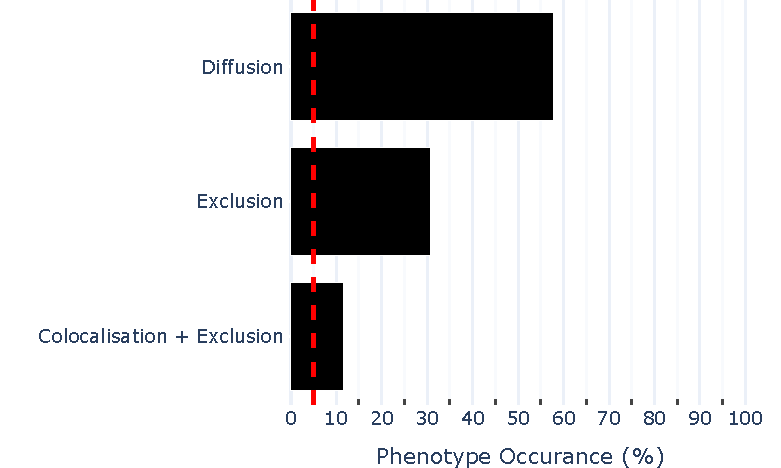
\includegraphics[width=1\linewidth]{09. Chapter 4/Figs/02. Overexpression/03. IFIT3/01. bar_i3_hrsv.pdf} 
    \end{subfigure}
    \begin{subfigure}{0.495\textwidth}
        \caption{}
        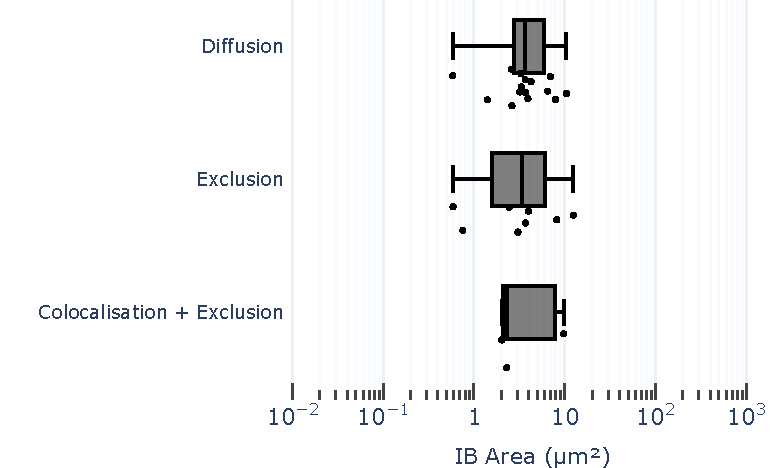
\includegraphics[width=1\linewidth]{09. Chapter 4/Figs/02. Overexpression/03. IFIT3/02. box_i3_hrsv.pdf}
    \end{subfigure}
    \caption[Observed Phenotypes of Exogenous bIFIT3 in the Context of hRSV Inclusion Bodies in Vero Cell Line.]{\textbf{Observed Phenotypes of Exogenous bIFIT3 in the Context of hRSV Inclusion Bodies in Vero Cell Line.} Vero cells were infected with human RSV at MOI 1. 24 HPI, the cells were transfected with bIFIT3-FLAG containing plasmids using TransIT-X2 and were fixed after further 24 hours. Cells were labeled with anti-RSV N and anti-FLAG antibodies and imaged on confocal microscope. Panel (a) shows percentual proportions of observed phenotypes between hRSV inclusion bodies and exogenous bIFIT3 (26 observations), with the red dotted line denoting the 5\% threshold, marking phenotypes considered relevant above this limit. Panel (b) shows the IB area in \(\mu \mbox{m}^2\) per observed relevant phenotype.}
    \label{fig:Observed Phenotypes of Exogenous bIFIT3 in the Context of hRSV Inclusion Bodies in VERO Cell Line}
\end{figure}

\begin{figure}
    \centering
    \includegraphics[width=1\linewidth]{09. Chapter 4/Figs/02. Overexpression/03. IFIT3/03. bi3-hrsv.pdf}
    \caption[Representative Images of Observed Phenotypes of Exogenous bIFIT3 in the Context of hRSV Inclusion Bodies in Vero Cell Line.]{\textbf{Representative Images of Observed Phenotypes of Exogenous bIFIT3 in the Context of hRSV Inclusion Bodies in Vero Cell Line.} Vero cells were infected with human RSV at MOI 1. 24 HPI, the cells were transfected with bIFIT3-FLAG containing plasmids using TransIT-X2 and were fixed after further 24 hours. Cellular nuclei were stained with DAPI (yellow), and cells were double-labeled with anti-RSV N (cyan) and anti-FLAG (magenta) antibodies. This figure showcases representative examples of relevant phenotypes in the interaction between exogenous bIFIT3 and hRSV inclusion bodies. These phenotypes are presented in descending order based on their percentage proportions. The scale bar indicates 2 \(\mu \mbox{m}\).}
    \label{fig:Representative Images of Observed Phenotypes of Exogenous bIFIT3 in the Context of hRSV Inclusion Bodies in VERO Cell Line}
\end{figure}

Next we set to nvestiigate the exogenous bovine IFIT3 intrreaction with hRSV IBs. Within 26 total observations we have identified 3 intreraction phenotypes, all of which occured above 5\% frequency. The respective phenotypes, ther frequences along with the mearured 2D area of the IBs is shown in Figure \ref{fig:Observed Phenotypes of Exogenous bIFIT3 in the Context of hRSV Inclusion Bodies in VERO Cell Line}. The representative images of these phenotypes are shown in Figure \ref{fig:Representative Images of Observed Phenotypes of Exogenous bIFIT3 in the Context of hRSV Inclusion Bodies in VERO Cell Line}. Unlike what we observed with human IFIT1, the predominant phenotypes do not imply interaction. The most comonly observed phenotype was diffusion (57\%), followed by exclusion (31\%), and colocalisaion associated with intra-IB exclusion (12\%). Although showing minute diffrences in the median observed IB sizes, all phenotypes were associated with almost identicaly sized IBs. In more detail diffusion-associated IBs ranged in size from 0.6 \(\mu \mbox{m}^2\) to supra 10 \(\mu \mbox{m}^2\), with the median value of 4 \(\mu \mbox{m}^2\). The size of exclusion-associated IBs also ranged from 0.6 \(\mu \mbox{m}^2\) to supra 10 \(\mu \mbox{m}^2\), but showed a typical value of 3.3 \(\mu \mbox{m}^2\). Lastly, the colocalisation associated with exclusion was observed to be associated with 3 IBs, which had sizes of 2 \(\mu \mbox{m}^2\), 2.1 \(\mu \mbox{m}^2\), and 10 \(\mu \mbox{m}^2\). This data suggest that these phenotypes occur independently of IB maturity. Interestingly we have failed to observe IBs with 2D areas above 10 \(\mu \mbox{m}^2\). This could be due to the the limited number of observations. It could also be explained by seemingly IB-intreaction independent anti-RSV action of bovine IFIT3, which limits the maximum size these structures can be.

\begin{figure}
    \begin{subfigure}{0.495\textwidth}
        \caption{}
        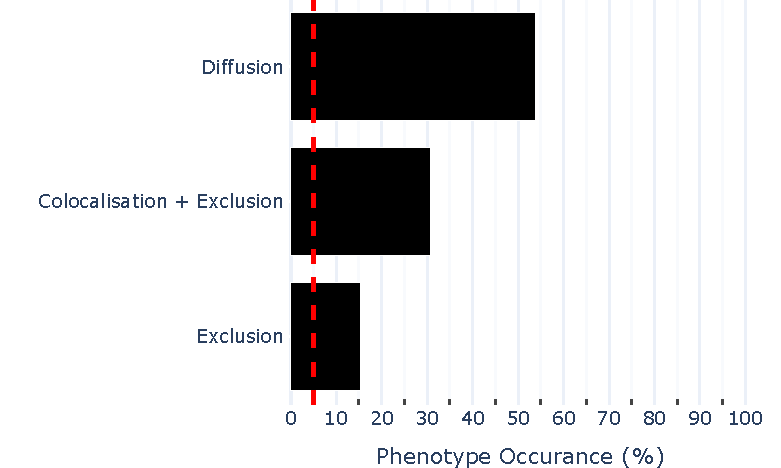
\includegraphics[width=1\linewidth]{09. Chapter 4/Figs/02. Overexpression/03. IFIT3/04. bar_i3_brsv.pdf} 
    \end{subfigure}
    \begin{subfigure}{0.495\textwidth}
        \caption{}
        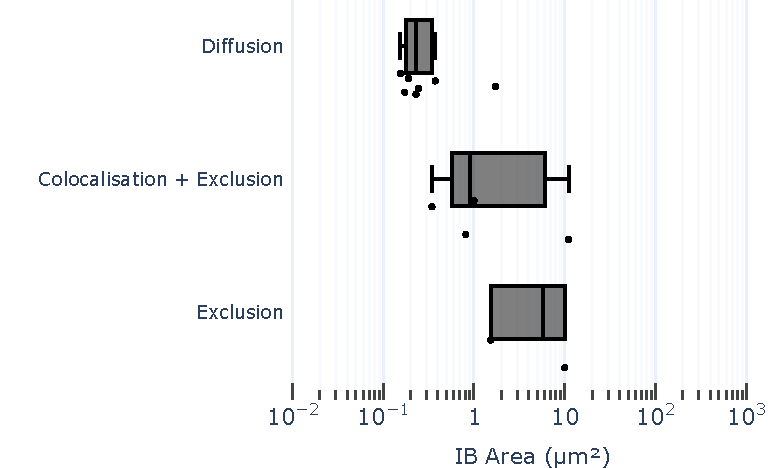
\includegraphics[width=1\linewidth]{09. Chapter 4/Figs/02. Overexpression/03. IFIT3/05. box_i3_brsv.pdf}
    \end{subfigure}
    \caption[Observed Phenotypes of Exogenous bIFIT3 in the Context of bRSV Inclusion Bodies in Vero Cell Line.]{\textbf{Observed Phenotypes of Exogenous bIFIT3 in the Context of bRSV Inclusion Bodies in Vero Cell Line.} Vero cells were infected with bovine RSV at MOI 1. 24 HPI, the cells were transfected with bIFIT3-FLAG containing plasmids using TransIT-X2 and were fixed after further 24 hours. Cells were labeled with anti-RSV N and anti-FLAG antibodies and imaged on confocal microscope. Panel (a) shows percentual proportions of observed phenotypes between bRSV inclusion bodies and exogenous bIFIT3 (13 observations), with the red dotted line denoting the 5\% threshold, marking phenotypes considered relevant above this limit. Panel (b) shows the IB area in \(\mu \mbox{m}^2\) per observed relevant phenotype.}
    \label{fig:Observed Phenotypes of Exogenous bIFIT3 in the Context of bRSV Inclusion Bodies in VERO Cell Line}
\end{figure}

\begin{figure}
    \centering
    \includegraphics[width=1\linewidth]{09. Chapter 4/Figs/02. Overexpression/03. IFIT3/06. bi3-brsv.pdf}
    \caption[Representative Images of Observed Phenotypes of Exogenous bIFIT3 in the Context of bRSV Inclusion Bodies in Vero Cell Line.]{\textbf{Representative Images of Observed Phenotypes of Exogenous bIFIT3 in the Context of bRSV Inclusion Bodies in Vero Cell Line.} Vero cells were infected with bovine RSV at MOI 1. 24 HPI, the cells were transfected with bIFIT3-FLAG containing plasmids using TransIT-X2 and were fixed after further 24 hours. Cellular nuclei were stained with DAPI (yellow), and cells were double-labeled with anti-RSV N (cyan) and anti-FLAG (magenta) antibodies. This figure showcases representative examples of relevant phenotypes in the interaction between exogenous bIFIT3 and bRSV inclusion bodies. These phenotypes are presented in descending order based on their percentage proportions. The scale bar indicates 2 \(\mu \mbox{m}\).}
    \label{fig:Representative Images of Observed Phenotypes of Exogenous bIFIT3 in the Context of bRSV Inclusion Bodies in VERO Cell Line}
\end{figure}

To validate the previous data and to establish if the seemingly non interactive nature of bovine IFIT3 with human IBs is due to the species difference we have set to investigate the interaction phenotypes between ectopicaly expressed bovine IFIT3 bRSV IBs. We obtained only 13 observations in ths analysis. The observed phenotypes along with their frequencies of occurance along with the IB sizes are shown in Figure \ref{fig:Observed Phenotypes of Exogenous bIFIT3 in the Context of bRSV Inclusion Bodies in VERO Cell Line}. The representative images of these phenotypes are shown in Figure \ref{fig:Representative Images of Observed Phenotypes of Exogenous bIFIT3 in the Context of bRSV Inclusion Bodies in VERO Cell Line}. In 54\% of observations we have observed bovine IFIT3 to be diffused throught the bRSV IBs. This was followed by colocalisation acompanied with excluision (31\%) and excluson (15\%) phenotypes. Unlike what was observed when we investigated the interaction of exogenous bIFIT3 with hRSV IBs, there seems to be a size distinction of IBs associated with the different phenotypes. The diffusion phenotype was observed predominantly in very small IBs, which size ranged from sub 0.2 \(\mu \mbox{m}^2\) to sub 2 \(\mu \mbox{m}^2\), with the median value of 0.9 \(\mu \mbox{m}^2\)where most of the IBs clustered. bIFIT3 was observed to colocalise with IB edge while beng excluded from ther centre of these structures in IBs with median size of 0.9 \(\mu \mbox{m}^2\). Lastly, the exclusion phenotype was associated with two IBs of sizes of 1.5 \(\mu \mbox{m}^2\) and 10 \(\mu \mbox{m}^2\). It is to be noted that the population of observed IBs is of a smaller size and we have failed to observe IBs with area larger than 10 \(\mu \mbox{m}^2\), which is unusual for 48 HPI RSV infection. This could be atreributed to the overall small amount of observations or to the potential IB interction-independent anti-RSV action of bovine IFIT3.







reasonably consistent results

minimal strong interaction phenotypes in infection (other than mdbk)

some strong interaction phenotypes in pIB

some strong interaction phenotypes in oe


very small ibs in oe so i3 could act ifit ndependently
small amount of direct interaction, maybe as a result of ifit123 formation?






\begin{figure}
    \begin{subfigure}{0.495\textwidth}
        \caption{}
        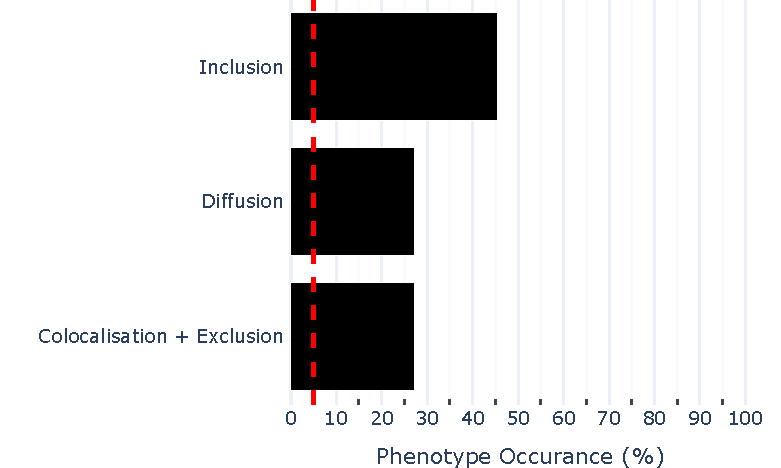
\includegraphics[width=1\linewidth]{09. Chapter 4/Figs/02. Overexpression/04. IFIT5/01. bar_i5_hrsv.pdf} 
    \end{subfigure}
    \begin{subfigure}{0.495\textwidth}
        \caption{}
        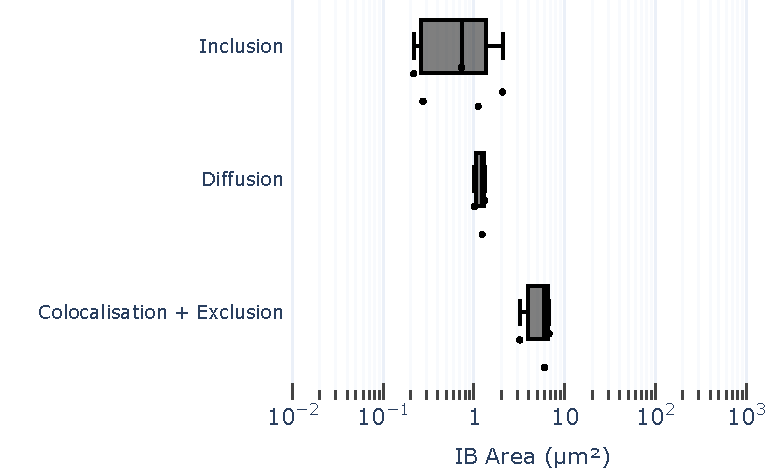
\includegraphics[width=1\linewidth]{09. Chapter 4/Figs/02. Overexpression/04. IFIT5/02. box_i5_hrsv.pdf}
    \end{subfigure}
    \caption[Observed Phenotypes of Exogenous hIFIT5 in the Context of hRSV Inclusion Bodies in Vero Cell Line.]{\textbf{Observed Phenotypes of Exogenous hIFIT5 in the Context of hRSV Inclusion Bodies in Vero Cell Line.} Vero cells were infected with human RSV at MOI 1. 24 HPI, the cells were transfected with hIFIT5-FLAG containing plasmids using TransIT-X2 and were fixed after further 24 hours. Cells were labeled with anti-RSV N and anti-FLAG antibodies and imaged on confocal microscope. Panel (a) shows percentual proportions of observed phenotypes between hRSV inclusion bodies and exogenous hIFIT5 (11 observations), with the red dotted line denoting the 5\% threshold, marking phenotypes considered relevant above this limit. Panel (b) shows the IB area in \(\mu \mbox{m}^2\) per observed relevant phenotype.}
    \label{fig:Observed Phenotypes of Exogenous hIFIT5 in the Context of hRSV Inclusion Bodies in VERO Cell Line}
\end{figure}

\begin{figure}
    \centering
    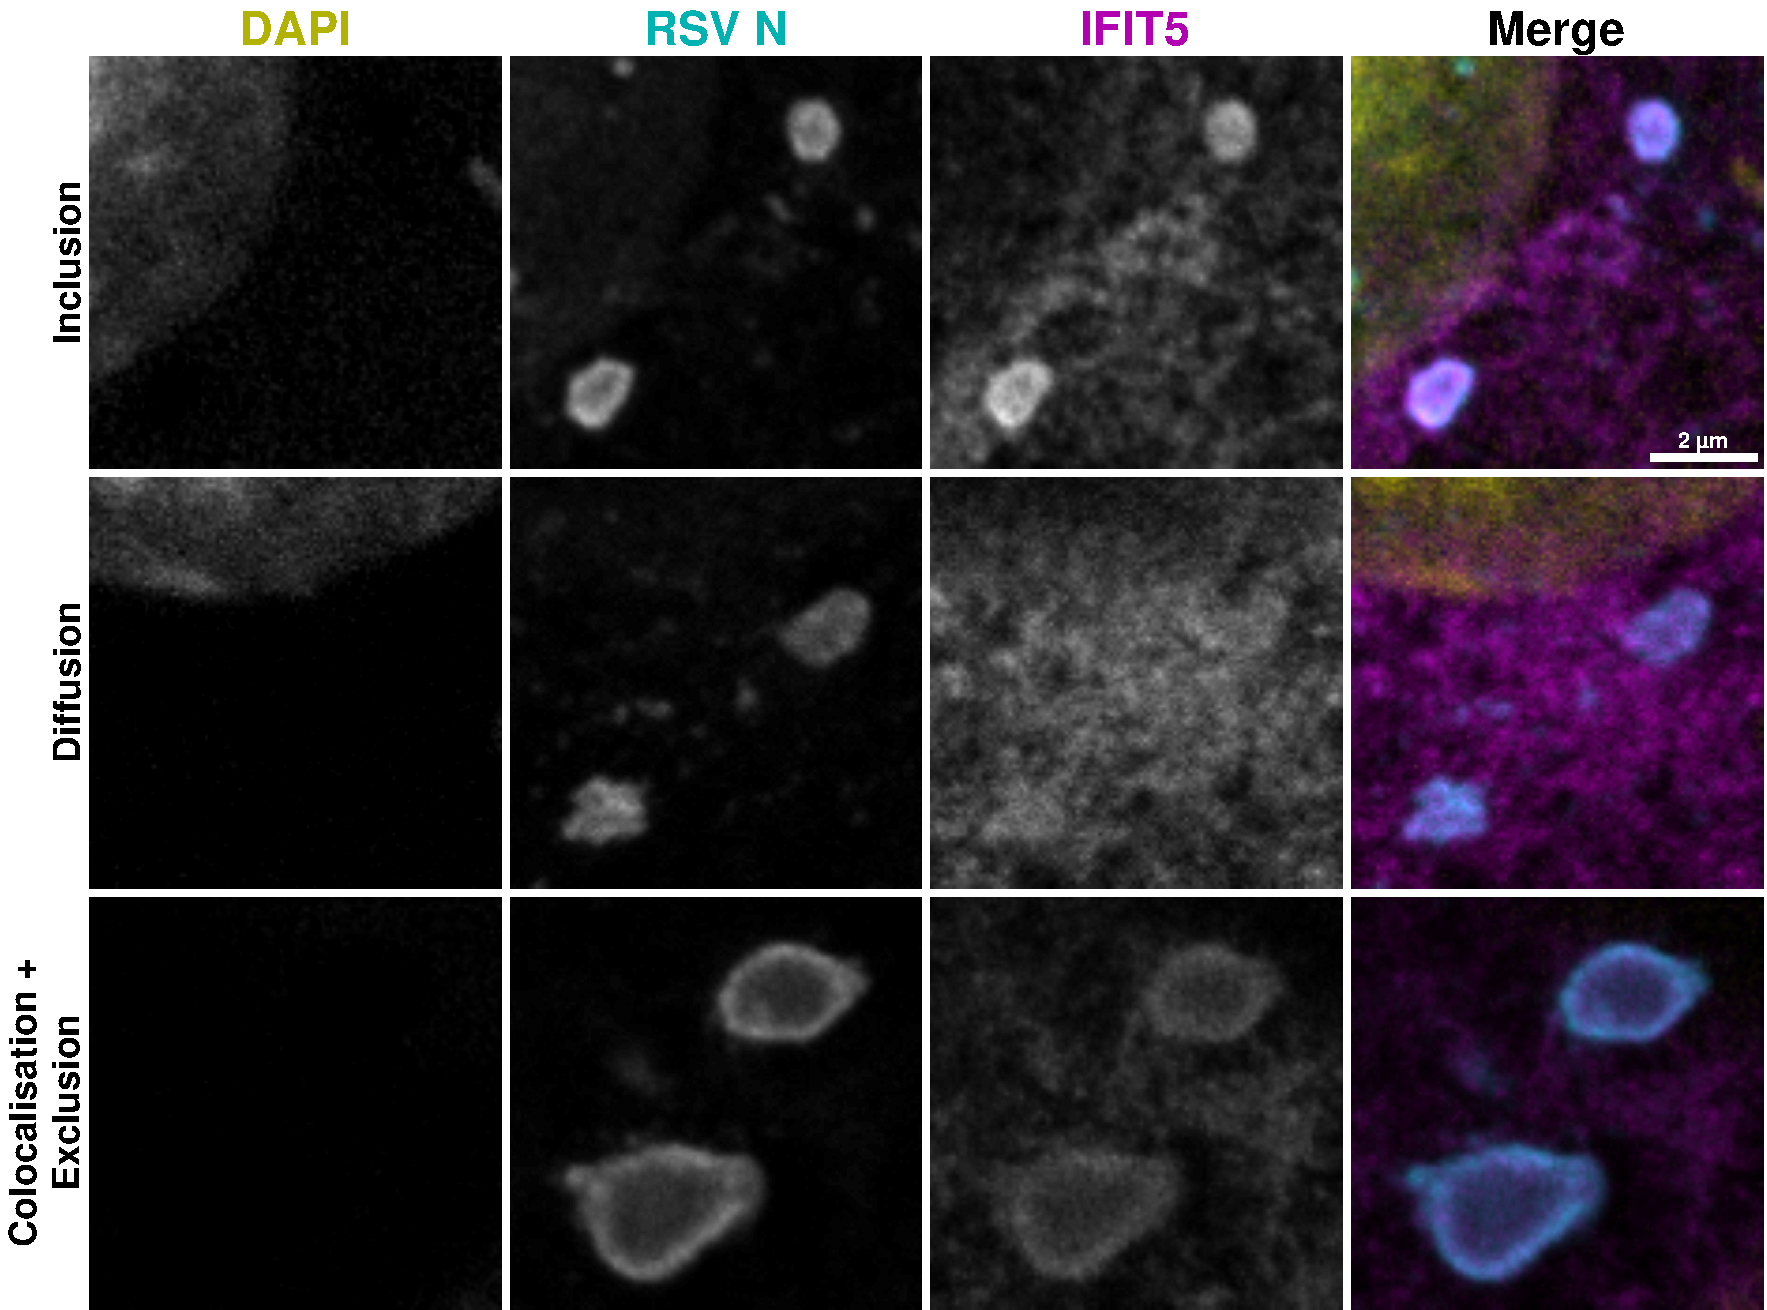
\includegraphics[width=1\linewidth]{09. Chapter 4/Figs/02. Overexpression/04. IFIT5/03. i5-hrsv.pdf}
    \caption[Representative Images of Observed Phenotypes of Exogenous hIFIT5 in the Context of hRSV Inclusion Bodies in Vero Cell Line.]{\textbf{Representative Images of Observed Phenotypes of Exogenous hIFIT5 in the Context of hRSV Inclusion Bodies in Vero Cell Line.} Vero cells were infected with human RSV at MOI 1. 24 HPI, the cells were transfected with hIFIT5-FLAG containing plasmids using TransIT-X2 and were fixed after further 24 hours. Cellular nuclei were stained with DAPI (yellow), and cells were double-labeled with anti-RSV N (cyan) and anti-FLAG (magenta) antibodies. This figure showcases representative examples of relevant phenotypes in the interaction between exogenous hIFIT5 and hRSV inclusion bodies. These phenotypes are presented in descending order based on their percentage proportions. The scale bar indicates 2 \(\mu \mbox{m}\).}
    \label{fig:Representative Images of Observed Phenotypes of Exogenous hIFIT5 in the Context of hRSV Inclusion Bodies in VERO Cell Line}
\end{figure}

Lastly we investigated the interaction of exogenously expressed human IFIT5 with hRSV IBs. We have collected 11 observations which showed 3 interaction phenotypes. These and their associated frequencies of occurances along with the measured IB sizes can be viewed in Figure \ref{fig:Observed Phenotypes of Exogenous hIFIT5 in the Context of hRSV Inclusion Bodies in VERO Cell Line}. The representative images of these phenotypes are shown in Figure \ref{fig:Representative Images of Observed Phenotypes of Exogenous hIFIT5 in the Context of hRSV Inclusion Bodies in VERO Cell Line}. The most comonly observed intreaction phenotype was intra-IB inclusion, which occured in 45\% of observations. This was followed by diffusion and colocalisation associated with exclusoion phenotypes, both of which accured in 26\% of observations. The inclusion phenotype occured in relatively small IBs, which ranged from sub 0.2 \(\mu \mbox{m}^2\) to 2 \(\mu \mbox{m}^2\) in size, with the median value of 0.7 \(\mu \mbox{m}^2\). The diffusion associated IBs toghtly clustered around their median size of 1.2 \(\mu \mbox{m}^2\). Lastly, the colocalisation associated with exclusion phenotype-associated IBs were larger in size, with a typical size of 6 \(\mu \mbox{m}^2\). It is evident that there is IB size-dependentr discintion of phenotypes. In small, sub 1 \(\mu \mbox{m}^2\) IBs human IFIT5 concentrates withing these structures. Asd the IBs increase in size and mature, the inclusion phenotype is maintaned, but also accompanied by diffusion phenotype. Lastly as the IBs further increase in size and reach the limt where IBAGs were reported to occur form the literature, human IFIT5 translocate from the IB interior to the IB boundry. It is to be noted that we have not observed IBs above 7 \(\mu \mbox{m}^2\) in size, suggesting yet again that we are dealing with a incomplete dataset or the increased concentraton of IFIT5 prevents larger IBs from forming.

\begin{figure}
    \begin{subfigure}{0.495\textwidth}
        \caption{}
        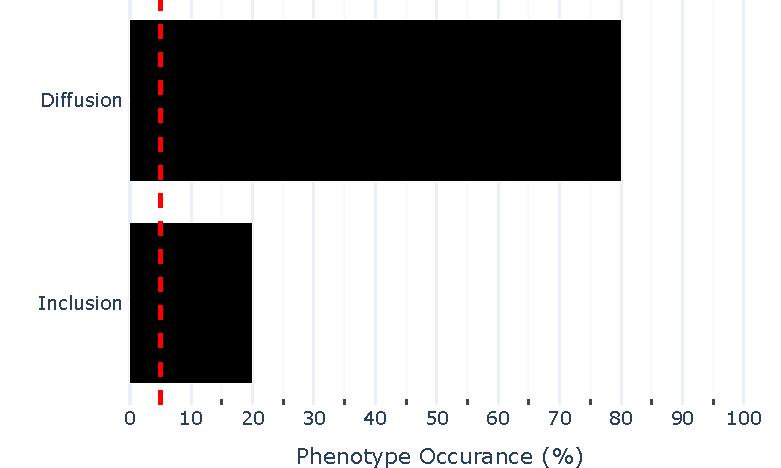
\includegraphics[width=1\linewidth]{09. Chapter 4/Figs/02. Overexpression/04. IFIT5/04. bar_i5_brsv.pdf} 
    \end{subfigure}
    \begin{subfigure}{0.495\textwidth}
        \caption{}
        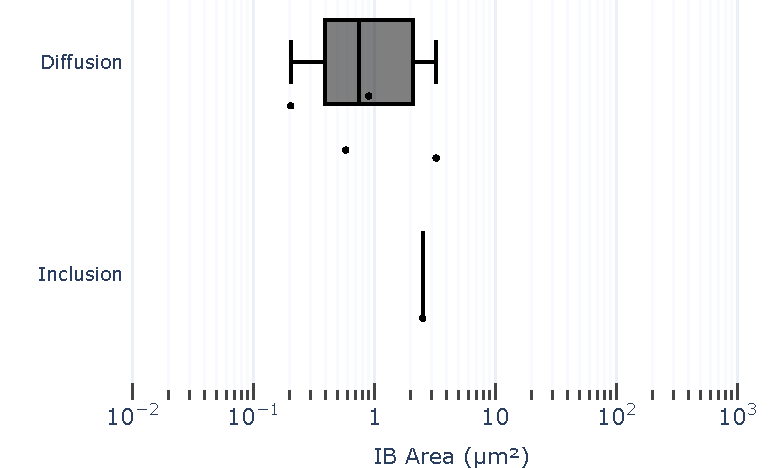
\includegraphics[width=1\linewidth]{09. Chapter 4/Figs/02. Overexpression/04. IFIT5/05. box_i5_brsv.pdf}
    \end{subfigure}
    \caption[Observed Phenotypes of Exogenous hIFIT5 in the Context of bRSV Inclusion Bodies in Vero Cell Line.]{\textbf{Observed Phenotypes of Exogenous hIFIT5 in the Context of bRSV Inclusion Bodies in Vero Cell Line.} Vero cells were infected with bovine RSV at MOI 1. 24 HPI, the cells were transfected with hIFIT5-FLAG containing plasmids using TransIT-X2 and were fixed after further 24 hours. Cells were labeled with anti-RSV N and anti-FLAG antibodies and imaged on confocal microscope. Panel (a) shows percentual proportions of observed phenotypes between bRSV inclusion bodies and exogenous hIFIT5 (5 observations), with the red dotted line denoting the 5\% threshold, marking phenotypes considered relevant above this limit. Panel (b) shows the IB area in \(\mu \mbox{m}^2\) per observed relevant phenotype.}
    \label{fig:Observed Phenotypes of Exogenous hIFIT5 in the Context of bRSV Inclusion Bodies in VERO Cell Line}
\end{figure}

\begin{figure}
    \centering
    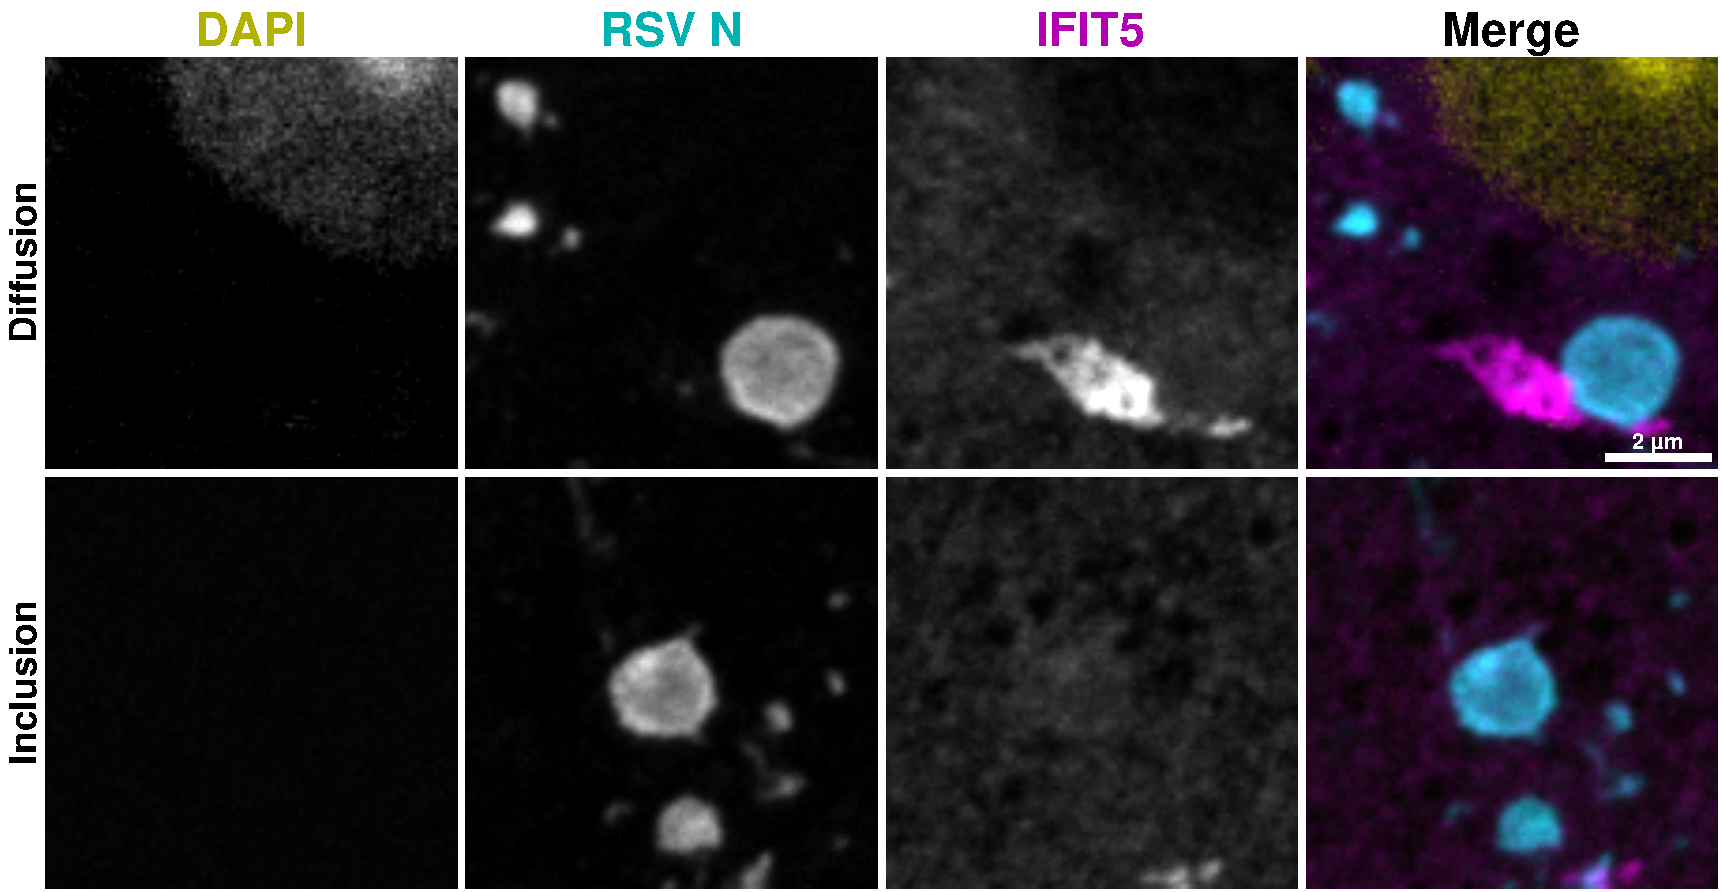
\includegraphics[width=1\linewidth]{09. Chapter 4/Figs/02. Overexpression/04. IFIT5/06. i5-brsv.pdf}
    \caption[Representative Images of Observed Phenotypes of Exogenous hIFIT5 in the Context of bRSV Inclusion Bodies in Vero Cell Line.]{\textbf{Representative Images of Observed Phenotypes of Exogenous hIFIT5 in the Context of bRSV Inclusion Bodies in Vero Cell Line.} Vero cells were infected with bovine RSV at MOI 1. 24 HPI, the cells were transfected with hIFIT5-FLAG containing plasmids using TransIT-X2 and were fixed after further 24 hours. Cellular nuclei were stained with DAPI (yellow), and cells were double-labeled with anti-RSV N (cyan) and anti-FLAG (magenta) antibodies. This figure showcases representative examples of relevant phenotypes in the interaction between exogenous hIFIT5 and bRSV inclusion bodies. These phenotypes are presented in descending order based on their percentage proportions. The scale bar indicates 2 \(\mu \mbox{m}\).}
    \label{fig:Representative Images of Observed Phenotypes of Exogenous hIFIT5 in the Context of bRSV Inclusion Bodies in VERO Cell Line}
\end{figure}

Finally we have investigated the intraction betwenn exogenously expressed human IFT5 and bRSV IBs. We have observed only 5 IB/IFIT5 interactions. Regardless, the observed phenotypes, their frequency of occurance, along with the measured IB areas are shown in Figure \ref{fig:Observed Phenotypes of Exogenous hIFIT5 in the Context of bRSV Inclusion Bodies in VERO Cell Line}, with the representative images of these phenotypes shown in Figure \ref{fig:Representative Images of Observed Phenotypes of Exogenous hIFIT5 in the Context of bRSV Inclusion Bodies in VERO Cell Line}. The most commonly occuring phenotypic interaction was diffusioin, which occured in 80\% of observations. IBs associated with this phenotype ranged from 0.2 \(\mu \mbox{m}^2\) to supra 3 \(\mu \mbox{m}^2\) in size, with the median measured area of 0.7 \(\mu \mbox{m}^2\). Following this we have observed one IB of 2.3 \(\mu \mbox{m}^2\) in size, inside which hIFIT5 was  observed to be concentrating and forming intra-IB inclusion. These seems to be a hint of phenotype separation based on IB size, similar to what we observed previoiously with hRSV infecton (Figure \ref{fig:Observed Phenotypes of Exogenous hIFIT5 in the Context of hRSV Inclusion Bodies in VERO Cell Line}), however this is difficult to completely assess based on 5 observations. Along this linesm we have failed to observe IBs larger than 4 \(\mu \mbox{m}^2\). Based on the hRSV results we hypothetise that these IBs would shown colocalisaton associated with exclusion phenotype.



infection mainly exclusion and edge exclusion (strong iinteraction >15\%)
mki5 + pib - only strong interacton

oe small amount of observations

i5 seems lke it can interact with these structures and does when OE
also possibly decreases the ib size
maybe not enough i5 during infection to do the effect

IFIT5 summary OE + pIB + infecton










final summary of all
\subsection{Dissecting the Differential IFIT2 Antibody Staining} \label{subsec:Dissecting the Differential IFIT2 Antibody Staining}
In Chapter \ref{ch:Subcellular Localisation of Endogenous IFIT Proteins in the Context of RSV Inclusion Bodies}, a striking differential staining pattern was observed between the two utilised anti-IFIT2 antibodies concerning the interaction of IFIT2 with human or bovine RSV inclusion bodies. The IFIT2(A) antibody revealed both human and bovine IFIT2 forming intra-IB inclusions in smaller IBs. Moreover, it observed IFIT2 to colocalise with the IB edge while being excluded from the IB centre in larger IBs. In contrast, IFIT2(B) predominantly detected IFIT2 to be excluded from IB structures, irrespective of IB size, occasionally showing IFIT2 to be equally distributed between the cytoplasm and IB structures. Additionally, a differential staining pattern was observed concerning the general subcellular localisation of IFIT2 in mock-treated cells, which was more pronounced in bovine cells. While both antibodies displayed general cytoplasmic staining of bovine IFIT2, IFIT2(A) staining revealed perinuclear concentrations resembling the Golgi apparatus. In contrast, IFIT2(B) antibody showed colocalisation of IFIT2 with the mitotic spindle. It appears that these two polyclonal antibodies are detecting two different entities, possibly two populations of IFIT2, basally present in both human and bovine cells. These populations may be detected by the antibodies based on differential epitope recognition. This difference could arise from one antibody detecting IFIT2 in complex with its interaction partners, such as IFIT1, IFIT3, MAVS, HOMER3, or double-stranded RNA, while the other antibody detects naked IFIT2 entities. The precise nature, however, remains to be elucidated.

To investigate this, we initially employed the same methodologies as were used in Section \ref{subsec:IFIT1, IFIT3, and IFIT5 Localisation with Regards to RSV Pseudo-IBs}. Specifically, we aimed to explore IFIT2 localisation concerning human and bovine RSV pseudo-inclusion bodies (pIBs), as detected by the IFIT2(A) and IFIT2(B) antibodies. We utilised the HEK293T and Vero cell lines to probe for endogenous human and monkey IFIT2, respectively. We induced hRSV pIBs in both HEK293T and Vero cell lines using the pcDNA3.1 plasmids containing ORFs for hRSV \textit{N} and \textit{P}. However, we encountered challenges in generating a sufficient amount of bRSV pIB-expressing Vero cells for staining with both IFIT2(A) and IFIT2(B) antibodies, and thus, the latter is missing from the analysis. This limitation may be attributed to contaminations in the plasmid preparations or a decrease in the quality of these plasmids.

\begin{figure}
    \centering
    \includegraphics[width=1\linewidth]{09. Chapter 4/Figs/01. pIB/03. IFIT2/01. Single Transfection/01. 293t-ifit2a.pdf}
    \caption[IFIT2(A) Antibody Detects Increased IFIT2 Expression Following hRSV P Transfection.]{\textbf{IFIT2(A) Antibody Detects Increased IFIT2 Expression Following hRSV P Transfection.} HEK293T cells were either mock transfected, or single transfected with empty vector, hRSV N containing plasmid, or hRSV P containing plasmid using TransIT-X2 and were fixed after 24 hours. Cellular nuclei were stained with DAPI (yellow), and cells were double-labelled with either anti-RSV N (cyan), or anti-RSV P (cyan) and anti-IFIT2(A) (magenta) antibodies. The scale bar indicates 50 \(\mu \mbox{m}\).}
    \label{fig:IFIT2(A) Antibody Detects Increased IFIT2 Expression Following hRSV P Transfection}
\end{figure}

\begin{figure}
    \centering
    \includegraphics[width=1\linewidth]{09. Chapter 4/Figs/01. pIB/03. IFIT2/01. Single Transfection/02. 293t-ifit2b.pdf}
    \caption[IFIT2(B) Antibody Does Not Detect Increased IFIT2 Expression Following hRSV P Transfection.]{\textbf{IFIT2(B) Antibody Does Not Detect Increased IFIT2 Expression Following hRSV P Transfection.} HEK293T cells were either mock transfected, or single transfected with empty vector, hRSV N containing plasmid, or hRSV P containing plasmid using TransIT-X2 and were fixed after 24 hours. Cellular nuclei were stained with DAPI (yellow), and cells were double-labelled with either anti-RSV N (cyan), or anti-RSV P (cyan) and anti-IFIT2(B) (magenta) antibodies. The scale bar indicates 50 \(\mu \mbox{m}\).}
    \label{fig:IFIT2(B) Antibody Does Not Detect Increased IFIT2 Expression Following hRSV P Transfection}
\end{figure}

During the fundamental control experiments, which involved assessing single RSV \textit{N} and \textit{P} transfections and transfections with an empty pcDNA3.1 plasmid, while comparing these to mock-transfected cells, we uncovered a differentiation between IFIT2(A) and IFIT2(B) staining. Notably, we observed IFIT2 induction in response to transfection with the hRSV \textit{P}-containing plasmid, a response not observed during transfection with the empty vector or the hRSV \textit{N}-containing plasmid. This induction was detected exclusively using IFIT2(A) (Figure \ref{fig:IFIT2(A) Antibody Detects Increased IFIT2 Expression Following hRSV P Transfection}), while IFIT2(B) staining did not reveal this phenotype (Figure \ref{fig:IFIT2(B) Antibody Does Not Detect Increased IFIT2 Expression Following hRSV P Transfection}). Similar control experiments for IFIT1, IFIT3, and IFIT5 yielded staining patterns consistent with the observations made with IFIT2(B) antibody (data not shown). Additionally, we observed differential subcellular localisation of IFIT2 between the two antibodies, consistent with the findings in Chapter \ref{ch:Subcellular Localisation of Endogenous IFIT Proteins in the Context of RSV Inclusion Bodies} in the MDBK cell line. IFIT2(A)-stained HEK293T mock cells showed perinuclear IFIT2 concentrations resembling lipid droplets or aggregosomes, based on definitions and examples provided by the Human Protein Atlas \cite{Thul2017AProteome}. In contrast, IFIT2(B) antibody revealed IFIT2 localising to the mitotic spindle. This data raises several questions. Firstly, given that \textit{IFIT} genes should share similar genomic regulation, the mechanism through which \textit{IFIT2} is induced following RSV \textit{P} exogenous expression needs clarification. Is this induction mediated directly by the action of the P protein, suggesting its relevance to infection? Such a scenario would imply a potential direct antiviral role of IFIT2 against RSV. Secondly, the apparent inability of IFIT2(B) antibody to detect this increased nascent IFIT2 prompts further inquiry. If the previously mentioned differential target epitope hypothesis based on IFIT2 interaction partners holds true, it suggests that IFIT2(B) antibody detects IFIT2 complexes and is thus blind to newly synthesised IFIT2, which has not yet formed these complexes. Additional experiments are warranted to validate this proposition.

\begin{figure}
    \begin{subfigure}{0.495\textwidth}
        \caption{}
        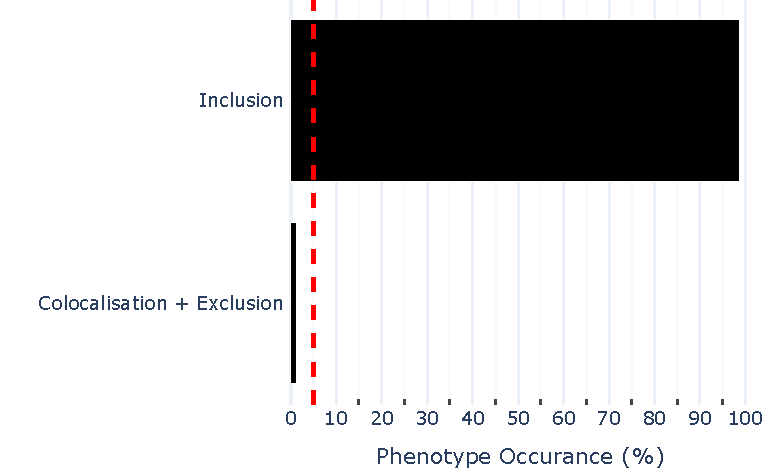
\includegraphics[width=1\linewidth]{09. Chapter 4/Figs/01. pIB/03. IFIT2/02. IFIT2A/01. bar_i2a_293t.pdf}
    \end{subfigure}
    \begin{subfigure}{0.495\textwidth}
        \caption{}
        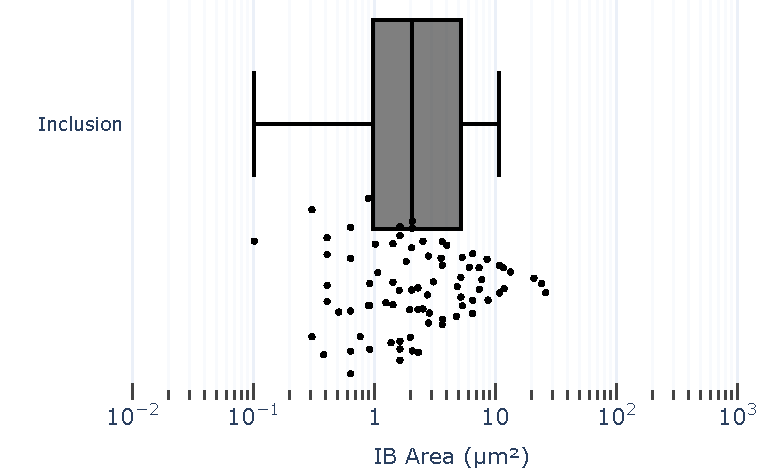
\includegraphics[width=1\linewidth]{09. Chapter 4/Figs/01. pIB/03. IFIT2/02. IFIT2A/02. box_i2a_293t.pdf}
    \end{subfigure}
    \caption[Observed Phenotypes of Endogenous Human IFIT2 in the Context of hRSV Pseudo Inclusion Bodies in 293T Cell Line, as Detected by IFIT2(A) Antibody.]{\textbf{Observed Phenotypes of Endogenous Human IFIT2 in the Context of hRSV Pseudo Inclusion Bodies in 293T Cell Line, as Detected by IFIT2(A) Antibody.} 293T cells were transfected with hRSV N and P containing plasmids using TransIT-X2 and were fixed after 24 hours. Cells were labelled with anti-RSV N and anti-IFIT2(A) antibodies and imaged on a confocal microscope. Panel (a) shows the percentual proportions of observed phenotypes between hRSV pseudo inclusion bodies and human IFIT2 (81 observations), with the red dotted line denoting the 5\% threshold, marking phenotypes considered relevant above this limit. Panel (b) shows the IB area in \(\mu \mbox{m}^2\) per observed relevant phenotype.}
    \label{fig:Observed Phenotypes of Endogenous Human IFIT2 in the Context of hRSV Pseudo Inclusion Bodies in 293T Cell Line, as Detected by IFIT2(A) Antibody}
\end{figure}

\begin{figure}
    \centering
    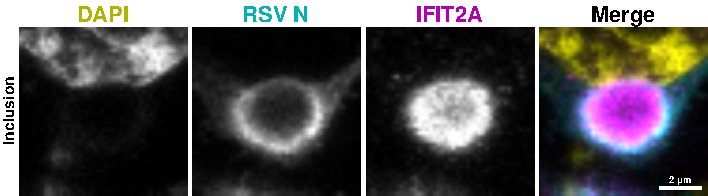
\includegraphics[width=1\linewidth]{09. Chapter 4/Figs/01. pIB/03. IFIT2/02. IFIT2A/03. i2a-293t-hnhp.pdf} 
    \caption[Representative Images of Observed Phenotypes of Endogenous Human IFIT2 in the Context of hRSV Pseudo Inclusion Bodies in 293T Cell Line, as Detected by IFIT2(A) Antibody.]{\textbf{Representative Images of Observed Phenotypes of Endogenous Human IFIT2 in the Context of hRSV Pseudo Inclusion Bodies in 293T Cell Line, as Detected by IFIT2(A) Antibody.} 293T cells were transfected with hRSV N and P containing plasmids using TransIT-X2 and were fixed after 24 hours. Cellular nuclei were stained with DAPI (yellow), and cells were double-labelled with anti-RSV N (cyan) and anti-IFIT2(A) (magenta) antibodies. This figure showcases representative examples of relevant phenotypes in the interaction between human IFIT2 and hRSV pseudo-inclusion bodies. These phenotypes are presented in descending order based on their percentage proportions. The scale bar indicates 2 \(\mu \mbox{m}\).}
    \label{fig:Representative Images of Observed Phenotypes of Endogenous Human IFIT2 in the Context of hRSV Pseudo Inclusion Bodies in 293T Cell Line, as Detected by IFIT2(A) Antibody}
\end{figure}

Next, we embarked on investigating the interaction phenotypes of IFIT2 with RSV pseudo IBs, as detected by the two antibodies. We initially focused on the signal identified by the IFIT2(A) antibody. We acquired 81 observations of human IFIT2 interacting with hRSV pIBs from the HEK293T cell line. Figure \ref{fig:Observed Phenotypes of Endogenous Human IFIT2 in the Context of hRSV Pseudo Inclusion Bodies in 293T Cell Line, as Detected by IFIT2(A) Antibody} displays the observed phenotypes, their frequencies of occurrences, and the pIB sizes associated with phenotypic interactions occurring with a frequency higher than 5\%. Representative images of phenotypes occurring at more than 5\% frequency are shown in Figure \ref{fig:Representative Images of Observed Phenotypes of Endogenous Human IFIT2 in the Context of hRSV Pseudo Inclusion Bodies in 293T Cell Line, as Detected by IFIT2(A) Antibody}. Predominantly, we observed IFIT2 forming intra-pIB inclusions, a phenotype occurring in 98\% of cases. In the remaining 2\% of observations, IFIT2 colocalised with the pIB boundary while being excluded from the pIB center. The sizes of inclusion-associated pIBs conformed to the general distribution of all observed pIBs in the HEK293T cell line, ranging from 0.1 \(\mu \mbox{m}^2\) to 25 \(\mu \mbox{m}^2\) in size, with a median area of 2 \(\mu \mbox{m}^2\). In contrast to observations with monkey IFIT1 and IFIT5, where the inclusion and colocalisation associated with exclusion phenotypes seemed to be restricted to small and large pIBs, respectively, we do not observe this distinction with endogenous human IFIT2. This suggests that IFIT2, as detected by the IFIT2(A) antibody, forms intra-pIB inclusions irrespective of their size.

\begin{figure}
    \begin{subfigure}{0.495\textwidth}
        \caption{}
        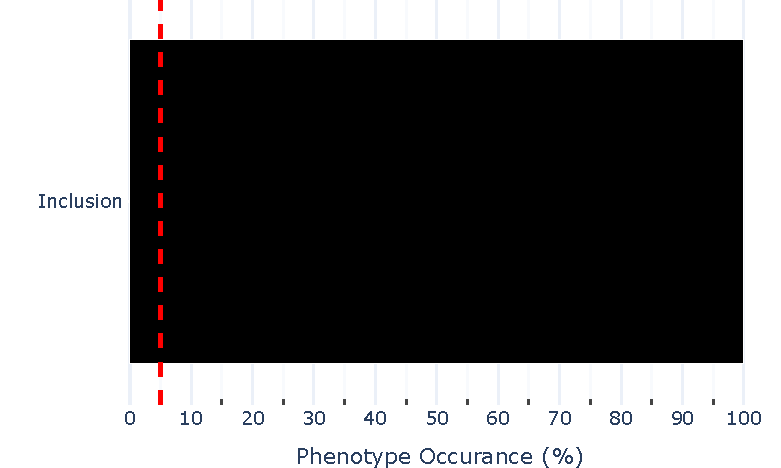
\includegraphics[width=1\linewidth]{09. Chapter 4/Figs/01. pIB/03. IFIT2/02. IFIT2A/04. bar_i2a_vero_hnhp.pdf} 
    \end{subfigure}
    \begin{subfigure}{0.495\textwidth}
        \caption{}
        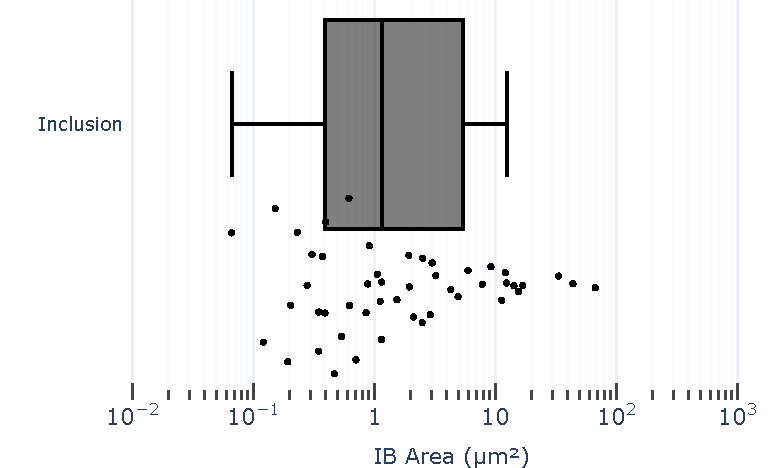
\includegraphics[width=1\linewidth]{09. Chapter 4/Figs/01. pIB/03. IFIT2/02. IFIT2A/05. box_i2a_vero_hnhp.pdf}
    \end{subfigure}
    \caption[Observed Phenotypes of Endogenous Monkey IFIT2 in the Context of hRSV Pseudo Inclusion Bodies in Vero Cell Line, as Detected by IFIT2(A) Antibody.]{\textbf{Observed Phenotypes of Endogenous Monkey IFIT2 in the Context of hRSV Pseudo Inclusion Bodies in Vero Cell Line, as Detected by IFIT2(A) Antibody.} Vero cells were transfected with hRSV N and P containing plasmids using TransIT-X2 and were fixed after 24 hours. Cells were labelled with anti-RSV N and anti-IFIT2(A) antibodies and imaged on a confocal microscope. Panel (a) shows the percentual proportions of observed phenotypes between hRSV pseudo inclusion bodies and monkey IFIT2 (48 observations), with the red dotted line denoting the 5\% threshold, marking phenotypes considered relevant above this limit. Panel (b) shows the IB area in \(\mu \mbox{m}^2\) per observed relevant phenotype.}
    \label{fig:Observed Phenotypes of Endogenous Monkey IFIT2 in the Context of hRSV Pseudo Inclusion Bodies in Vero Cell Line, as Detected by IFIT2(A) Antibody}
\end{figure}

\begin{figure}
    \centering
    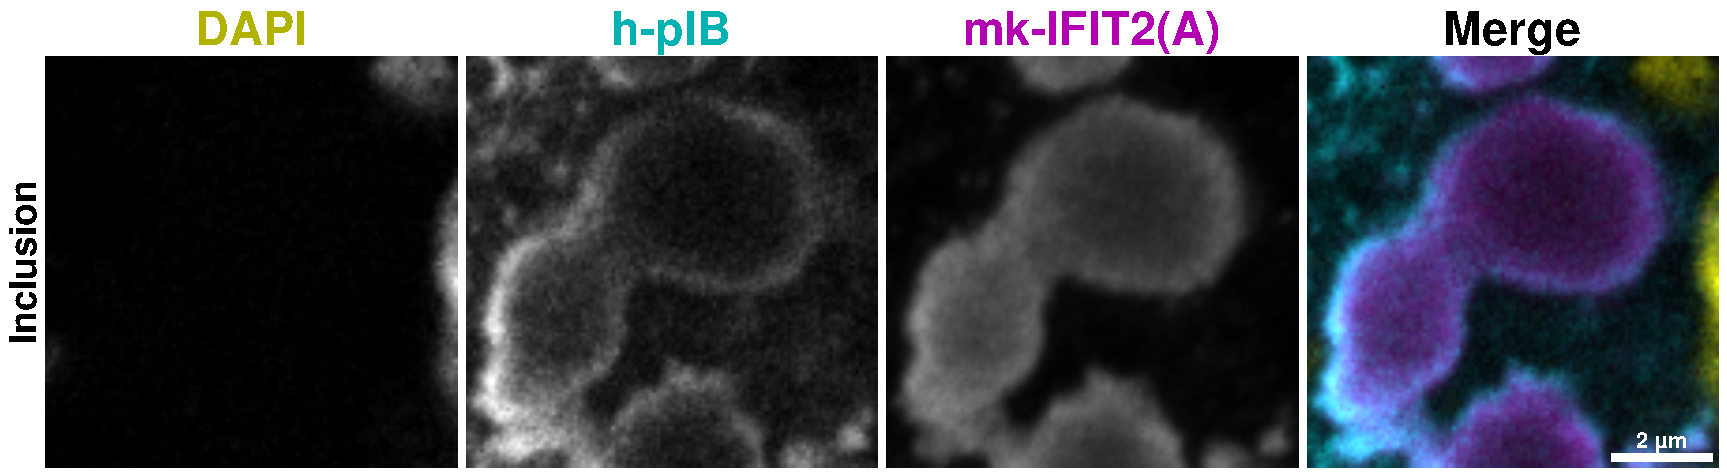
\includegraphics[width=1\linewidth]{09. Chapter 4/Figs/01. pIB/03. IFIT2/02. IFIT2A/06. i2a-vero-hnhp.pdf}  
    \caption[Representative Images of Observed Phenotypes of Endogenous Monkey IFIT2 in the Context of hRSV Pseudo Inclusion Bodies in Vero Cell Line, as Detected by IFIT2(A) Antibody.]{\textbf{Representative Images of Observed Phenotypes of Endogenous Monkey IFIT2 in the Context of hRSV Pseudo Inclusion Bodies in Vero Cell Line, as Detected by IFIT2(A) Antibody.} Vero cells were transfected with hRSV N and P containing plasmids using TransIT-X2 and were fixed after 24 hours. Cellular nuclei were stained with DAPI (yellow), and cells were double-labelled with anti-RSV N (cyan) and anti-IFIT2(A) (magenta) antibodies. This figure showcases representative examples of relevant phenotypes in the interaction between monkey IFIT2 and hRSV pseudo-inclusion bodies. These phenotypes are presented in descending order based on their percentage proportions. The scale bar indicates 2 \(\mu \mbox{m}\).}
    \label{fig:Representative Images of Observed Phenotypes of Endogenous Monkey IFIT2 in the Context of hRSV Pseudo Inclusion Bodies in Vero Cell Line, as Detected by IFIT2(A) Antibody}
\end{figure}

Further, we examined the interaction between monkey IFIT2 and hRSV pIBs using the IFIT2(A) antibody. To accomplish this, we transfected Vero cells with plasmids containing hRSV \textit{N} and \textit{P}. We obtained 48 observations, all of which conformed to the inclusion phenotype (Figure \ref{fig:Observed Phenotypes of Endogenous Monkey IFIT2 in the Context of hRSV Pseudo Inclusion Bodies in Vero Cell Line, as Detected by IFIT2(A) Antibody}, panel a). The measured area of these hRSV pIBs is shown in Figure \ref{fig:Observed Phenotypes of Endogenous Monkey IFIT2 in the Context of hRSV Pseudo Inclusion Bodies in Vero Cell Line, as Detected by IFIT2(A) Antibody}, panel b. The representative image is displayed in Figure \ref{fig:Representative Images of Observed Phenotypes of Endogenous Monkey IFIT2 in the Context of hRSV Pseudo Inclusion Bodies in Vero Cell Line, as Detected by IFIT2(A) Antibody}. The distribution of the pIB sizes is almost identical to the aggregate dataset of all pIBs observed in the Vero cell line, ranging from sub 0.07 \(\mu \mbox{m}^2\) to supra 60 \(\mu \mbox{m}^2\), with a typical value of 1.2 \(\mu \mbox{m}^2\). This data is consistent with our observations in HEK293T cells.

\begin{figure}
    \begin{subfigure}{0.495\textwidth}
        \caption{}
        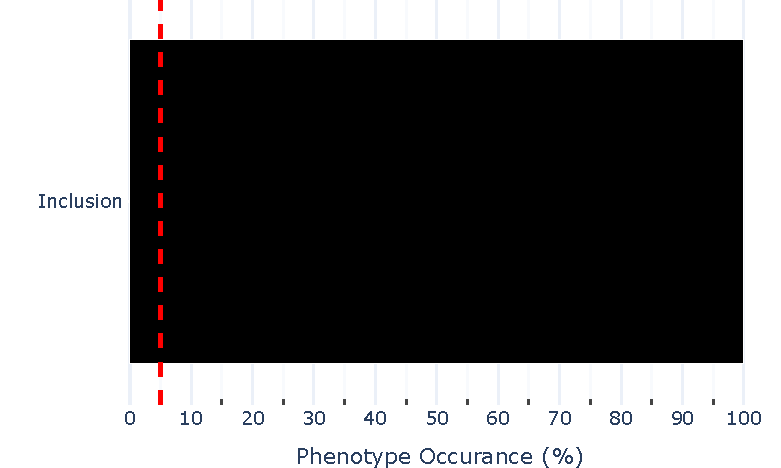
\includegraphics[width=1\linewidth]{09. Chapter 4/Figs/01. pIB/03. IFIT2/02. IFIT2A/07. bar_i2a_vero_bnbp.pdf} 
    \end{subfigure}
    \begin{subfigure}{0.495\textwidth}
        \caption{}
        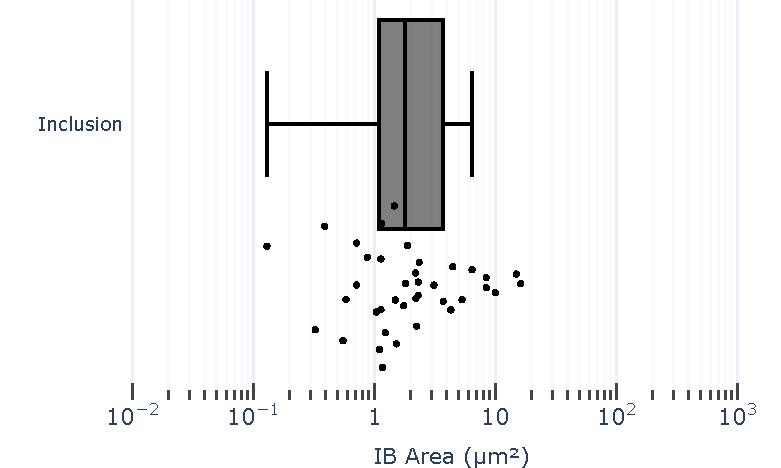
\includegraphics[width=1\linewidth]{09. Chapter 4/Figs/01. pIB/03. IFIT2/02. IFIT2A/08. box_i2a_vero_bnbp.pdf}
    \end{subfigure}
    \caption[Observed Phenotypes of Endogenous Monkey IFIT2 in the Context of bRSV Pseudo Inclusion Bodies in Vero Cell Line, as Detected by IFIT2(A) Antibody.]{\textbf{Observed Phenotypes of Endogenous Monkey IFIT2 in the Context of bRSV Pseudo Inclusion Bodies in Vero Cell Line, as Detected by IFIT2(A) Antibody.} Vero cells were transfected with bRSV N and P containing plasmids using TransIT-X2 and were fixed after 24 hours. Cells were labelled with anti-RSV N and anti-IFIT2(A) antibodies and imaged on a confocal microscope. Panel (a) shows the percentual proportions of observed phenotypes between bRSV pseudo inclusion bodies and monkey IFIT2 (38 observations), with the red dotted line denoting the 5\% threshold, marking phenotypes considered relevant above this limit. Panel (b) shows the IB area in \(\mu \mbox{m}^2\) per observed relevant phenotype.}
    \label{fig:Observed Phenotypes of Endogenous Monkey IFIT2 in the Context of bRSV Pseudo Inclusion Bodies in Vero Cell Line, as Detected by IFIT2(A) Antibody}
\end{figure}

\begin{figure}
    \centering
    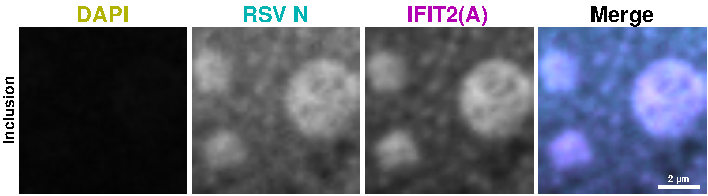
\includegraphics[width=1\linewidth]{09. Chapter 4/Figs/01. pIB/03. IFIT2/02. IFIT2A/09. i2a-vero-bnbp.pdf} 
    \caption[Representative Images of Observed Phenotypes of Endogenous Monkey IFIT2 in the Context of bRSV Pseudo Inclusion Bodies in Vero Cell Line, as Detected by IFIT2(A) Antibody.]{\textbf{Representative Images of Observed Phenotypes of Endogenous Monkey IFIT2 in the Context of bRSV Pseudo Inclusion Bodies in Vero Cell Line, as Detected by IFIT2(A) Antibody.} Vero cells were transfected with bRSV N and P containing plasmids using TransIT-X2 and were fixed after 24 hours. Cellular nuclei were stained with DAPI (yellow), and cells were double-labelled with anti-RSV N (cyan) and anti-IFIT2(A) (magenta) antibodies. This figure showcases representative examples of relevant phenotypes in the interaction between monkey IFIT2 and bRSV pseudo-inclusion bodies. These phenotypes are presented in descending order based on their percentage proportions. The scale bar indicates 2 \(\mu \mbox{m}\).}
    \label{fig:Representative Images of Observed Phenotypes of Endogenous Monkey IFIT2 in the Context of bRSV Pseudo Inclusion Bodies in Vero Cell Line, as Detected by IFIT2(A) Antibody}
\end{figure}

Finally, we explored the interaction between monkey IFIT2 and bRSV pIBs using the IFIT2(A) antibody. This involved the transfection of Vero cells with bRSV \textit{N} and \textit{P} containing plasmids, resulting in 38 observations, all of which displayed the inclusion phenotype (Figure \ref{fig:Observed Phenotypes of Endogenous Monkey IFIT2 in the Context of bRSV Pseudo Inclusion Bodies in Vero Cell Line, as Detected by IFIT2(A) Antibody}, panel a). The measured area of these bRSV pIBs is illustrated in Figure \ref{fig:Observed Phenotypes of Endogenous Monkey IFIT2 in the Context of bRSV Pseudo Inclusion Bodies in Vero Cell Line, as Detected by IFIT2(A) Antibody}, panel b. Additionally, a representative image is provided in Figure \ref{fig:Representative Images of Observed Phenotypes of Endogenous Monkey IFIT2 in the Context of bRSV Pseudo Inclusion Bodies in Vero Cell Line, as Detected by IFIT2(A) Antibody}. While the observed pIBs may not perfectly represent the entirety of pIB observations in the Vero cell line, they span a significant range of pIB sizes. Consequently, we can confidently conclude that monkey IFIT2 forms intra-pIB inclusions regardless of the pIB's size. Specifically, these observed pIBs vary in size from 0.12 \(\mu \mbox{m}^2\) to 16 \(\mu \mbox{m}^2\), with a median value of 1.8 \(\mu \mbox{m}^2\). In summary, the IFIT2(A) antibody consistently detects IFIT2 forming intra-pIB inclusions, demonstrating the robustness of this interaction across different host cells, viral species, and pIB sizes.

\begin{figure}
    \begin{subfigure}{0.495\textwidth}
        \caption{}
        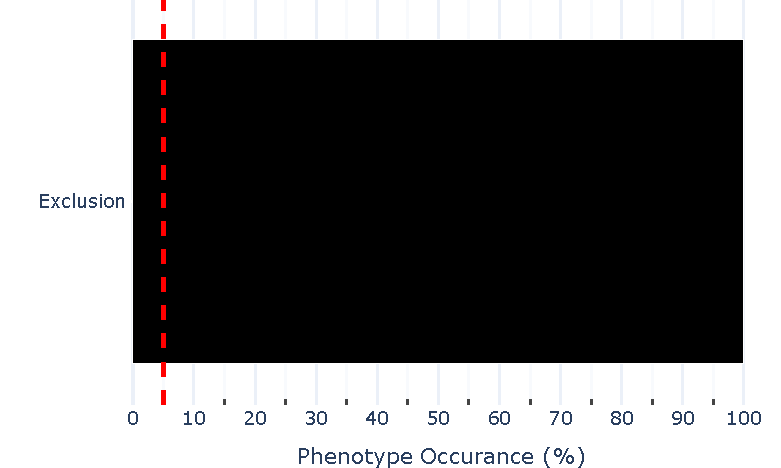
\includegraphics[width=1\linewidth]{09. Chapter 4/Figs/01. pIB/03. IFIT2/03. IFIT2B/01. bar_i2b_293t.pdf} 
    \end{subfigure}
    \begin{subfigure}{0.495\textwidth}
        \caption{}
        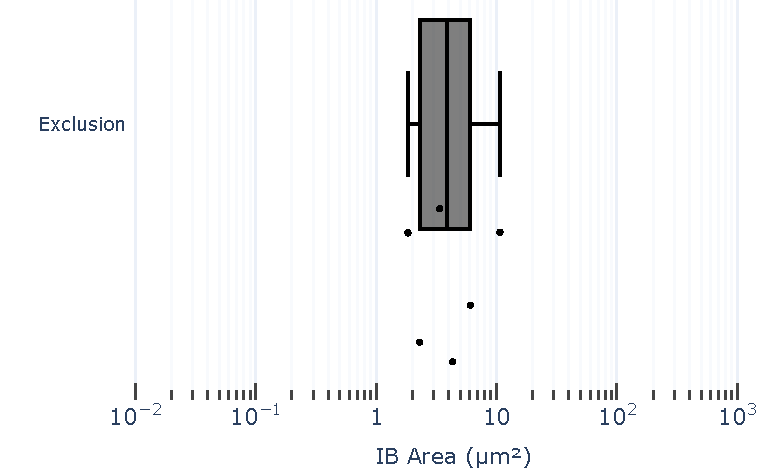
\includegraphics[width=1\linewidth]{09. Chapter 4/Figs/01. pIB/03. IFIT2/03. IFIT2B/02. box_i2b_293t.pdf}
    \end{subfigure}
    \caption[Observed Phenotypes of Endogenous Human IFIT2 in the Context of hRSV Pseudo Inclusion Bodies in 293T Cell Line, as Detected by IFIT2(B) Antibody.]{\textbf{Observed Phenotypes of Endogenous Human IFIT2 in the Context of hRSV Pseudo Inclusion Bodies in 293T Cell Line, as Detected by IFIT2(B) Antibody.} 293T cells were transfected with hRSV N and P containing plasmids using TransIT-X2 and were fixed after 24 hours. Cells were labelled with anti-RSV N and anti-IFIT2(B) antibodies and imaged on a confocal microscope. Panel (a) shows the percentual proportions of observed phenotypes between hRSV pseudo inclusion bodies and human IFIT2 (6 observations), with the red dotted line denoting the 5\% threshold, marking phenotypes considered relevant above this limit. Panel (b) shows the IB area in \(\mu \mbox{m}^2\) per observed relevant phenotype.}
    \label{fig:Observed Phenotypes of Endogenous Human IFIT2 in the Context of hRSV Pseudo Inclusion Bodies in 293T Cell Line, as Detected by IFIT2(B) Antibody}
\end{figure}

\begin{figure}
    \centering
    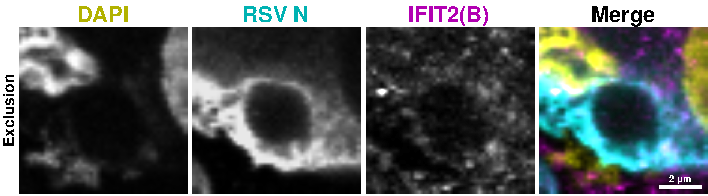
\includegraphics[width=1\linewidth]{09. Chapter 4/Figs/01. pIB/03. IFIT2/03. IFIT2B/03. i2b-293t-hnhp.pdf} 
    \caption[Representative Images of Observed Phenotypes of Endogenous Human IFIT2 in the Context of hRSV Pseudo Inclusion Bodies in 293T Cell Line, as Detected by IFIT2(B) Antibody.]{\textbf{Representative Images of Observed Phenotypes of Endogenous Human IFIT2 in the Context of hRSV Pseudo Inclusion Bodies in 293T Cell Line, as Detected by IFIT2(B) Antibody.} 293T cells were transfected with hRSV N and P containing plasmids using TransIT-X2 and were fixed after 24 hours. Cellular nuclei were stained with DAPI (yellow), and cells were double-labelled with anti-RSV N (cyan) and anti-IFIT2(B) (magenta) antibodies. This figure showcases representative examples of relevant phenotypes in the interaction between human IFIT2 and hRSV pseudo-inclusion bodies. These phenotypes are presented in descending order based on their percentage proportions. The scale bar indicates 2 \(\mu \mbox{m}\).}
    \label{fig:Representative Images of Observed Phenotypes of Endogenous Human IFIT2 in the Context of hRSV Pseudo Inclusion Bodies in 293T Cell Line, as Detected by IFIT2(B) Antibody}
\end{figure}

Next, we directed our attention to assessing the interaction of IFIT2 with hRSV pIBs, as detected by the IFIT2(B) antibody. Initially, we investigated the interaction of human IFIT2 with hRSV pIBs obtained from the HEK293T cell line. However, we obtained only 6 observations, all of which exhibited an exclusion phenotype (Figure \ref{fig:Observed Phenotypes of Endogenous Human IFIT2 in the Context of hRSV Pseudo Inclusion Bodies in 293T Cell Line, as Detected by IFIT2(B) Antibody}, panel a). The measured area of these hRSV pIBs is displayed in Figure \ref{fig:Observed Phenotypes of Endogenous Human IFIT2 in the Context of hRSV Pseudo Inclusion Bodies in 293T Cell Line, as Detected by IFIT2(B) Antibody}, panel b. The representative image of this phenotype is presented in Figure \ref{fig:Representative Images of Observed Phenotypes of Endogenous Human IFIT2 in the Context of hRSV Pseudo Inclusion Bodies in 293T Cell Line, as Detected by IFIT2(B) Antibody}. Although the observed pIBs were limited to 6, they encompass the range where the majority of the total observed hRSV pIB sizes were situated, ranging from sub 2 \(\mu \mbox{m}^2\) to supra 10 \(\mu \mbox{m}^2\), with a typical value of 4 \(\mu \mbox{m}^2\).

\begin{figure}
    \begin{subfigure}{0.495\textwidth}
        \caption{}
        \includegraphics[width=1\linewidth]{09. Chapter 4/Figs/01. pIB/03. IFIT2/03. IFIT2B/04. bar_i2b_vero_hnhp.pdf} 
    \end{subfigure}
    \begin{subfigure}{0.495\textwidth}
        \caption{}
        \includegraphics[width=1\linewidth]{09. Chapter 4/Figs/01. pIB/03. IFIT2/03. IFIT2B/05. box_i2b_vero_hnhp.pdf}
    \end{subfigure}
    \caption[Observed Phenotypes of Endogenous Monkey IFIT2 in the Context of hRSV Pseudo Inclusion Bodies in Vero Cell Line, as Detected by IFIT2(B) Antibody.]{\textbf{Observed Phenotypes of Endogenous Monkey IFIT2 in the Context of hRSV Pseudo Inclusion Bodies in Vero Cell Line, as Detected by IFIT2(B) Antibody.} Vero cells were transfected with hRSV N and P containing plasmids using TransIT-X2 and were fixed after 24 hours. Cells were labelled with anti-RSV N and anti-IFIT2(B) antibodies and imaged on a confocal microscope. Panel (a) shows the percentual proportions of observed phenotypes between hRSV pseudo inclusion bodies and monkey IFIT2 (76 observations), with the red dotted line denoting the 5\% threshold, marking phenotypes considered relevant above this limit. Panel (b) shows the IB area in \(\mu \mbox{m}^2\) per observed relevant phenotype.}
    \label{fig:Observed Phenotypes of Endogenous Monkey IFIT2 in the Context of hRSV Pseudo Inclusion Bodies in Vero Cell Line, as Detected by IFIT2(B) Antibody}
\end{figure}

\begin{figure}
    \centering
    \includegraphics[width=1\linewidth]{09. Chapter 4/Figs/01. pIB/03. IFIT2/03. IFIT2B/06. i2b-vero-hnhp.pdf} 
    \caption[Representative Images of Observed Phenotypes of Endogenous Monkey IFIT2 in the Context of hRSV Pseudo Inclusion Bodies in Vero Cell Line, as Detected by IFIT2(B) Antibody.]{\textbf{Representative Images of Observed Phenotypes of Endogenous Monkey IFIT2 in the Context of hRSV Pseudo Inclusion Bodies in Vero Cell Line, as Detected by IFIT2(B) Antibody.} Vero cells were transfected with hRSV N and P containing plasmids using TransIT-X2 and were fixed after 24 hours. Cellular nuclei were stained with DAPI (yellow), and cells were double-labelled with anti-RSV N (cyan) and anti-IFIT2(B) (magenta) antibodies. This figure showcases representative examples of relevant phenotypes in the interaction between monkey IFIT2 and hRSV pseudo-inclusion bodies. These phenotypes are presented in descending order based on their percentage proportions. The scale bar indicates 2 \(\mu \mbox{m}\).}
    \label{fig:Representative Images of Observed Phenotypes of Endogenous Monkey IFIT2 in the Context of hRSV Pseudo Inclusion Bodies in Vero Cell Line, as Detected by IFIT2(B) Antibody}
\end{figure}

Finally, we examined the interaction of endogenous monkey IFIT2 with hRSV pIBs, as detected by the IFIT2(B) antibody. Figure \ref{fig:Observed Phenotypes of Endogenous Monkey IFIT2 in the Context of hRSV Pseudo Inclusion Bodies in Vero Cell Line, as Detected by IFIT2(B) Antibody} presents the observed interaction phenotypes, their respective frequencies of occurrence, and the associated pIB sizes denoted per observed phenotype. Representative images of these interactions are shown in Figure \ref{fig:Representative Images of Observed Phenotypes of Endogenous Monkey IFIT2 in the Context of hRSV Pseudo Inclusion Bodies in Vero Cell Line, as Detected by IFIT2(B) Antibody}. Among the 76 observations, two phenotypes were identified: exclusion and diffusion. The former was predominant, appearing in 91\% of observations, while the latter occurred in 9\% of cases. The exclusion phenotype spanned a wide range of pIB sizes, representative of the aggregate distribution of all pIB sizes detected in the Vero cell line. Specifically, they ranged from 0.2 \(\mu \mbox{m}^2\) to 21 \(\mu \mbox{m}^2\), with a typical size of 2 \(\mu \mbox{m}^2\). The diffusion phenotype, however, predominantly occurred in smaller pIBs, ranging from 0.43 \(\mu \mbox{m}^2\) to 1 \(\mu \mbox{m}^2\), with a median size of 0.63 \(\mu \mbox{m}^2\).

Overall, our observations of IFIT2 interaction with RSV pIBs were consistent with those observed with endogenous human and bovine IFIT2 during RSV infection in Section \ref{subsec:Endogenous IFIT Interaction with RSV Inclusion Bodies}. The IFIT2(B) antibody detected endogenous human and monkey IFIT2 to be excluded from hRSV pIBs, with the exception of monkey IFIT2, where diffusion was also observed in 9\% of cases. In contrast, the IFIT2(A) antibody detected IFIT2 forming intra-pIBs solely, regardless of the host species or the species of the virus from which the pIBs originated. This differs from our observations during infection, where both human and bovine IFIT2, as detected by the IFIT2(A) antibody, were observed to form intra-IB inclusions in smaller IBs and to colocalise with the IB edge while being excluded from the IB interior in larger IBs. Nevertheless, a distinct difference is evident in observed IFIT2 using the two antibodies, and further investigation is needed to understand the nature of the differences observed by these antibodies. Employing a distinct epitope, such as the FLAG tag, could enhance our confidence in detecting the entire IFIT2 population.

To address this, we utilised the human IFIT2-FLAG-containing plasmid, provided by the Viral Gene Expression group at the Pirbright Institute, and the bovine IFIT2-FLAG-containing plasmid, prepared as described in Section \ref{sec:DNA Work} and Section \ref{subsec:Overexpressed IFIT1, IFIT3, and IFIT5 During RSV Infection}. We chose to initially assess these in the context of human and bovine RSV pseudo-inclusion bodies, as these yielded more defined interaction phenotypes as detected by the IFIT2(A) and IFIT2(B) antibodies. This approach also offers higher transfection efficiency compared to co-infection/transfection. After overexpressing the FLAG-tagged IFIT2, we aimed not only to probe the FLAG tag to obtain ground truth about IFIT2 subcellular localisation with respect to RSV pIBs but also to probe with the IFIT2(A) and IFIT2(B) antibodies to determine if their differential IFIT2 detection remains unchanged.

\begin{figure}
    \begin{subfigure}{0.495\textwidth}
        \caption{}
        \includegraphics[width=1\linewidth]{09. Chapter 4/Figs/01. pIB/03. IFIT2/04. IFIT2-FLAG/01. IFIT2A/01. bar_i2a_hnhp.pdf} 
    \end{subfigure}
    \begin{subfigure}{0.495\textwidth}
        \caption{}
        \includegraphics[width=1\linewidth]{09. Chapter 4/Figs/01. pIB/03. IFIT2/04. IFIT2-FLAG/01. IFIT2A/02. box_i2a_hnhp.pdf}
    \end{subfigure}
    \caption[Observed Phenotypes of Exogenous Human IFIT2 in the Context of hRSV Pseudo Inclusion Bodies in Vero Cell Line, as Detected by IFIT2(A) Antibody.]{\textbf{Observed Phenotypes of Exogenous Human IFIT2 in the Context of hRSV Pseudo Inclusion Bodies in Vero Cell Line, as Detected by IFIT2(A) Antibody.} Vero cells were transfected with hRSV N and P, along with human IFIT2-FLAG containing plasmids using TransIT-X2 and were fixed after 24 hours. Cells were labelled with anti-RSV N and anti-IFIT2(A) antibodies and imaged on a confocal microscope. Panel (a) shows the percentual proportions of observed phenotypes between hRSV pseudo inclusion bodies and exogenous human IFIT2 (56 observations), with the red dotted line denoting the 5\% threshold, marking phenotypes considered relevant above this limit. Panel (b) shows the IB area in \(\mu \mbox{m}^2\) per observed relevant phenotype.}
    \label{fig:Observed Phenotypes of Exogenous Human IFIT2 in the Context of hRSV Pseudo Inclusion Bodies in Vero Cell Line, as Detected by IFIT2(A) Antibody}
\end{figure}

\begin{figure}
    \centering
    \includegraphics[width=1\linewidth]{09. Chapter 4/Figs/01. pIB/03. IFIT2/04. IFIT2-FLAG/01. IFIT2A/03. i2a-hi2f-hnhp.pdf}
    \caption[Representative Images of Observed Phenotypes of Exogenous Human IFIT2 in the Context of hRSV Pseudo Inclusion Bodies in Vero Cell Line, as Detected by IFIT2(A) Antibody.]{\textbf{Representative Images of Observed Phenotypes of Exogenous Human IFIT2 in the Context of hRSV Pseudo Inclusion Bodies in Vero Cell Line, as Detected by IFIT2(A) Antibody.} Vero cells were transfected with hRSV N and P, along with human IFIT2-FLAG containing plasmids using TransIT-X2 and were fixed after 24 hours. Cellular nuclei were stained with DAPI (yellow), and cells were double-labelled with anti-RSV N (cyan) and anti-IFIT2(A) (magenta) antibodies. This figure showcases representative examples of relevant phenotypes in the interaction between exogenous human IFIT2 and hRSV pseudo-inclusion bodies. These phenotypes are presented in descending order based on their percentage proportions. The scale bar indicates 2 \(\mu \mbox{m}\).}
    \label{fig:Representative Images of Observed Phenotypes of Exogenous Human IFIT2 in the Context of hRSV Pseudo Inclusion Bodies in Vero Cell Line, as Detected by IFIT2(A) Antibody}
\end{figure}

Initially, we expressed human IFIT2-FLAG in the context of hRSV pseudo-IBs in the Vero cell line and detected IFIT2 using the IFIT2(A) antibody. Successful transfection of hIFIT2-FLAG was determined by an increased IFIT2 signal compared to the surrounding cells (data not shown). We observed 56 instances, all displaying the inclusion phenotype (Figure \ref{fig:Observed Phenotypes of Exogenous Human IFIT2 in the Context of hRSV Pseudo Inclusion Bodies in Vero Cell Line, as Detected by IFIT2(A) Antibody}, panel a). The observed pIBs ranged in size from 0.09 \(\mu \mbox{m}^2\) to 29 \(\mu \mbox{m}^2\), with a median value of 0.9 \(\mu \mbox{m}^2\) (Figure \ref{fig:Observed Phenotypes of Exogenous Human IFIT2 in the Context of hRSV Pseudo Inclusion Bodies in Vero Cell Line, as Detected by IFIT2(A) Antibody}, panel b). Notably, we observed IFIT2 forming inclusions within nuclear pIBs as well, a phenomenon which will be described in more detail below. The representative images of cellular and nuclear inclusions are presented in Figure \ref{fig:Representative Images of Observed Phenotypes of Exogenous Human IFIT2 in the Context of hRSV Pseudo Inclusion Bodies in Vero Cell Line, as Detected by IFIT2(A) Antibody}.

\begin{figure}
    \begin{subfigure}{0.495\textwidth}
        \caption{}
        \includegraphics[width=1\linewidth]{09. Chapter 4/Figs/01. pIB/03. IFIT2/04. IFIT2-FLAG/02. IFIT2B/01. bar_i2b_hnhp.pdf}
    \end{subfigure}
    \begin{subfigure}{0.495\textwidth}
        \caption{}
        \includegraphics[width=1\linewidth]{09. Chapter 4/Figs/01. pIB/03. IFIT2/04. IFIT2-FLAG/02. IFIT2B/02. box_i2a_hnhp.pdf}
    \end{subfigure}
    \caption[Observed Phenotypes of Exogenous Human IFIT2 in the Context of hRSV Pseudo Inclusion Bodies in Vero Cell Line, as Detected by IFIT2(B) Antibody.]{\textbf{Observed Phenotypes of Exogenous Human IFIT2 in the Context of hRSV Pseudo Inclusion Bodies in Vero Cell Line, as Detected by IFIT2(B) Antibody.} Vero cells were transfected with hRSV N and P, along with human IFIT2-FLAG containing plasmids using TransIT-X2 and were fixed after 24 hours. Cells were labelled with anti-RSV N and anti-IFIT2(B) antibodies and imaged on a confocal microscope. Panel (a) shows the percentual proportions of observed phenotypes between hRSV pseudo inclusion bodies and exogenous human IFIT2 (44 observations), with the red dotted line denoting the 5\% threshold, marking phenotypes considered relevant above this limit. Panel (b) shows the IB area in \(\mu \mbox{m}^2\) per observed relevant phenotype.}
    \label{fig:Observed Phenotypes of Exogenous Human IFIT2 in the Context of hRSV Pseudo Inclusion Bodies in Vero Cell Line, as Detected by IFIT2(B) Antibody}
\end{figure}

\begin{figure}
    \centering
    \includegraphics[width=1\linewidth]{09. Chapter 4/Figs/01. pIB/03. IFIT2/04. IFIT2-FLAG/02. IFIT2B/03. i2b-hi2f-hnhp.pdf}
    \caption[Representative Images of Observed Phenotypes of Exogenous Human IFIT2 in the Context of hRSV Pseudo Inclusion Bodies in Vero Cell Line, as Detected by IFIT2(B) Antibody.]{\textbf{Representative Images of Observed Phenotypes of Exogenous Human IFIT2 in the Context of hRSV Pseudo Inclusion Bodies in Vero Cell Line, as Detected by IFIT2(B) Antibody.} Vero cells were transfected with hRSV N and P, along with human IFIT2-FLAG containing plasmids using TransIT-X2 and were fixed after 24 hours. Cellular nuclei were stained with DAPI (yellow), and cells were double-labelled with anti-RSV N (cyan) and anti-IFIT2(B) (magenta) antibodies. This figure showcases representative examples of relevant phenotypes in the interaction between exogenous human IFIT2 and hRSV pseudo-inclusion bodies. These phenotypes are presented in descending order based on their percentage proportions. The scale bar indicates 2 \(\mu \mbox{m}\).}
    \label{fig:Representative Images of Observed Phenotypes of Exogenous Human IFIT2 in the Context of hRSV Pseudo Inclusion Bodies in Vero Cell Line, as Detected by IFIT2(B) Antibody}
\end{figure}

Next, we replicated the previous experiment using the IFIT2(B) antibody for the detection of exogenous human IFIT2-FLAG. We obtained 44 observations of IFIT2-pIB interactions. The observed interactions, their frequencies of occurrence, along with the pIB sizes associated with phenotypes occurring with more than 5\% frequency, are illustrated in Figure \ref{fig:Observed Phenotypes of Exogenous Human IFIT2 in the Context of hRSV Pseudo Inclusion Bodies in Vero Cell Line, as Detected by IFIT2(B) Antibody}. Representative images of these interactions are shown in Figure \ref{fig:Representative Images of Observed Phenotypes of Exogenous Human IFIT2 in the Context of hRSV Pseudo Inclusion Bodies in Vero Cell Line, as Detected by IFIT2(B) Antibody}. Surprisingly, the most common interaction phenotype was inclusion, occurring in half of the observations. This was closely followed by the exclusion phenotype, which occurred in 47\% of cases. Lastly, we observed 3\% of observations conforming to the diffusion phenotype. While the inclusion phenotype occurred in pIBs of a broad size range, from 0.21 \(\mu \mbox{m}^2\) to 7.2 \(\mu \mbox{m}^2\), with a median value of 3.2 \(\mu \mbox{m}^2\), the exclusion phenotype occurred predominantly in smaller pIBs, ranging from sub 0.2 \(\mu \mbox{m}^2\) to 3.5 \(\mu \mbox{m}^2\), with a median value of 0.4 \(\mu \mbox{m}^2\). We observed the exclusion-associated pIBs to be located within the boundary of a nucleus. Taken together, both IFIT2(A) and IFIT2(B) antibodies detect exogenously expressed hIFIT2-FLAG forming intra-pIB inclusions. However, a discrepancy persists between the antibodies; IFIT2(A) detected IFIT2 forming inclusions within nuclear pIBs, while IFIT2(B) antibody observed IFIT2 to be excluded from these. Both antibodies did not detect IFIT2 within the nucleoplasm. Due to the persistent differential staining of the two antibodies, it is imperative to probe the exogenous IFIT2 using the anti-FLAG antibody.

\begin{figure}
    \begin{subfigure}{0.495\textwidth}
        \caption{}
        \includegraphics[width=1\linewidth]{09. Chapter 4/Figs/01. pIB/03. IFIT2/04. IFIT2-FLAG/03. FLAG/01. bar_hi2f_hnhp.pdf}
    \end{subfigure}
    \begin{subfigure}{0.495\textwidth}
        \caption{}
        \includegraphics[width=1\linewidth]{09. Chapter 4/Figs/01. pIB/03. IFIT2/04. IFIT2-FLAG/03. FLAG/02. box_hi2f_hnhp.pdf}
    \end{subfigure}
    \caption[Observed Phenotypes of Exogenous Human IFIT2 in the Context of hRSV Pseudo Inclusion Bodies in Vero Cell Line, as Detected by FLAG Antibody.]{\textbf{Observed Phenotypes of Exogenous Human IFIT2 in the Context of hRSV Pseudo Inclusion Bodies in Vero Cell Line, as Detected by FLAG Antibody.} Vero cells were transfected with hRSV N and P, along with human IFIT2-FLAG containing plasmids using TransIT-X2 and were fixed after 24 hours. Cells were labelled with anti-RSV N and anti-FLAG antibodies and imaged on a confocal microscope. Panel (a) shows the percentual proportions of observed phenotypes between hRSV pseudo inclusion bodies and exogenous human IFIT2 (116 observations), with the red dotted line denoting the 5\% threshold, marking phenotypes considered relevant above this limit. Panel (b) shows the IB area in \(\mu \mbox{m}^2\) per observed relevant phenotype.}
    \label{fig:Observed Phenotypes of Exogenous Human IFIT2 in the Context of hRSV Pseudo Inclusion Bodies in Vero Cell Line, as Detected by FLAG Antibody}
\end{figure}

\begin{figure}
    \centering
    \includegraphics[width=1\linewidth]{09. Chapter 4/Figs/01. pIB/03. IFIT2/04. IFIT2-FLAG/03. FLAG/03. hi2f-hnhp.pdf}
    \caption[Representative Images of Observed Phenotypes of Exogenous Human IFIT2 in the Context of hRSV Pseudo Inclusion Bodies in Vero Cell Line, as Detected by FLAG Antibody.]{\textbf{Representative Images of Observed Phenotypes of Exogenous Human IFIT2 in the Context of hRSV Pseudo Inclusion Bodies in Vero Cell Line, as Detected by FLAG Antibody.} Vero cells were transfected with hRSV N and P, along with human IFIT2-FLAG containing plasmids using TransIT-X2 and were fixed after 24 hours. Cellular nuclei were stained with DAPI (yellow), and cells were double-labelled with anti-RSV N (cyan) and anti-FLAG (magenta) antibodies. This figure showcases representative examples of relevant phenotypes in the interaction between exogenous human IFIT2 and hRSV pseudo-inclusion bodies. These phenotypes are presented in descending order based on their percentage proportions. The scale bar indicates 2 \(\mu \mbox{m}\).}
    \label{fig:Representative Images of Observed Phenotypes of Exogenous Human IFIT2 in the Context of hRSV Pseudo Inclusion Bodies in Vero Cell Line, as Detected by FLAG Antibody}
\end{figure}

Using the anti-FLAG antibody, we probed the true localisation of exogenously expressed human IFIT2-FLAG and its interaction with hRSV pIBs. The frequencies of occurrences of observed interaction phenotypes, based on 116 observations, along with the measured pIB sizes associated with the phenotypes, are depicted in Figure \ref{fig:Observed Phenotypes of Exogenous Human IFIT2 in the Context of hRSV Pseudo Inclusion Bodies in Vero Cell Line, as Detected by FLAG Antibody}. Representative images of these phenotypes are shown in Figure \ref{fig:Representative Images of Observed Phenotypes of Exogenous Human IFIT2 in the Context of hRSV Pseudo Inclusion Bodies in Vero Cell Line, as Detected by FLAG Antibody}. The most common phenotype was exclusion from the pIB structures, occurring in 49\% of observations. This was followed by intra-pIB inclusions, occurring at a frequency of 35\%. Lastly, we detected IFIT2 to be diffused equally throughout the cytoplasm and the pIB structure in 21\% of observations. Exclusion appeared predominantly in smaller sub 1 \(\mu \mbox{m}^2\) pIBs, although we observed 4 pIBs associated with this phenotype that were larger than this. In more detail, exclusion-associated pIBs ranged from 0.09 \(\mu \mbox{m}^2\) to 9 \(\mu \mbox{m}^2\), with a typical value of 0.23 \(\mu \mbox{m}^2\). These pIBs were also located within the boundary of the nucleus. The inclusion-associated pIBs ranged from 0.2 \(\mu \mbox{m}^2\) to 9 \(\mu \mbox{m}^2\), with a median value of 2.1 \(\mu \mbox{m}^2\). Lastly, while the diffusion phenotype occurred predominantly with small, sub 1 \(\mu \mbox{m}^2\) pIBs, we observed 6 outliers that were each progressively larger. In general, the diffusion-associated pIBs ranged from 0.09 \(\mu \mbox{m}^2\) to 55 \(\mu \mbox{m}^2\), with a median value of just 0.7 \(\mu \mbox{m}^2\).

These data are consistent with what was observed in overexpressed hIFIT2-FLAG as detected by the IFIT2(B) antibody, suggesting that this antibody more realistically portrays the IFIT2 population. It is intriguing that ectopic expression of IFIT2 suddenly enables the IFIT2(B) antibody to detect IFIT2 forming intra-pIB inclusions. This observation is difficult to explain, but we suspect it may result from exogenous IFIT2-FLAG losing some of its interaction partners, potentially due to the C-terminal FLAG tag. This data also indicates that our previous assumption was correct, meaning the real interaction of IFIT2 with both IB and pIB involves both exclusion and strong interaction phenotypes (inclusion or colocalisation associated with exclusion), occurring approximately in the same frequency. Another intriguing fact is that while both IFIT2(B) and FLAG antibodies did not detect IFIT2 interaction with the nucleus-associated pIBs, the IFIT2(A) antibody was able to detect inclusions. This could possibly be explained by IFIT2(A) off-target effects or by some mechanism which we do not comprehend yet.

\begin{figure}
    \begin{subfigure}{0.495\textwidth}
        \caption{}
        \includegraphics[width=1\linewidth]{09. Chapter 4/Figs/01. pIB/03. IFIT2/04. IFIT2-FLAG/03. FLAG/04. bar_bi2f_hnhp.pdf} 
    \end{subfigure}
    \begin{subfigure}{0.495\textwidth}
        \caption{}
        \includegraphics[width=1\linewidth]{09. Chapter 4/Figs/01. pIB/03. IFIT2/04. IFIT2-FLAG/03. FLAG/05. box_bi2f_hnhp.pdf}
    \end{subfigure}
    \caption[Observed Phenotypes of Exogenous Bovine IFIT2 in the Context of hRSV Pseudo Inclusion Bodies in Vero Cell Line, as Detected by FLAG Antibody.]{\textbf{Observed Phenotypes of Exogenous Bovine IFIT2 in the Context of hRSV Pseudo Inclusion Bodies in Vero Cell Line, as Detected by FLAG Antibody.} Vero cells were transfected with hRSV N (or N-GFP) and P, along with bovine IFIT2-FLAG containing plasmids using TransIT-X2 and were fixed after 24 hours. Cells were labelled with anti-RSV N and anti-FLAG antibodies and imaged on a confocal microscope. The N-GFP containing pIBs were visualised using the innate fluorescence of the GFP. Panel (a) shows the percentual proportions of observed phenotypes between hRSV pseudo inclusion bodies and exogenous bovine IFIT2 (142 observations), with the red dotted line denoting the 5\% threshold, marking phenotypes considered relevant above this limit. Panel (b) shows the IB area in \(\mu \mbox{m}^2\) per observed relevant phenotype.}
    \label{fig:Observed Phenotypes of Exogenous Bovine IFIT2 in the Context of hRSV Pseudo Inclusion Bodies in Vero Cell Line, as Detected by FLAG Antibody}
\end{figure}

\begin{figure}
    \centering
    \includegraphics[width=1\linewidth]{09. Chapter 4/Figs/01. pIB/03. IFIT2/04. IFIT2-FLAG/03. FLAG/06. bi2f-hnhp.pdf}
    \caption[Representative Images of Observed Phenotypes of Exogenous Bovine IFIT2 in the Context of hRSV Pseudo Inclusion Bodies in Vero Cell Line, as Detected by FLAG Antibody.]{\textbf{Representative Images of Observed Phenotypes of Exogenous Bovine IFIT2 in the Context of hRSV Pseudo Inclusion Bodies in Vero Cell Line, as Detected by FLAG Antibody.} Vero cells were transfected with hRSV N (or N-GFP) and P, along with bovine IFIT2-FLAG containing plasmids using TransIT-X2 and were fixed after 24 hours. Cellular nuclei were stained with DAPI (yellow), and cells were double-labelled with anti-RSV N (cyan) and anti-FLAG (magenta) antibodies. The N-GFP containing pIBs were visualised using the innate fluorescence of the GFP (colocalisation + exclusion phenotype). This figure showcases representative examples of relevant phenotypes in the interaction between exogenous bovine IFIT2 and hRSV pseudo-inclusion bodies. These phenotypes are presented in descending order based on their percentage proportions. The scale bar indicates 2 \(\mu \mbox{m}\).}
    \label{fig:Representative Images of Observed Phenotypes of Exogenous Bovine IFIT2 in the Context of hRSV Pseudo Inclusion Bodies in Vero Cell Line, as Detected by FLAG Antibody}
\end{figure}

We continued the investigation of IFIT2-FLAG interaction with pIB structures, focusing solely on the FLAG antibody for detection. Attempts to obtain data from exogenous human IFIT2-FLAG with regards to bRSV pIBs were unsuccessful, as we failed to detect a single cell co-transfected by all three required plasmids. Consequently, we proceeded with the investigation involving exogenously expressed bovine IFIT2-FLAG in the context of human and bovine RSV pseudo-inclusion bodies. Firstly, we explored overexpressed bIFIT2-FLAG and its interaction with hRSV pIBs induced by co-transfecting RSV \textit{P}-containing plasmid with either hRSV \textit{N}- or \textit{N-GFP}-containing plasmids. The GFP signal, which is more sensitive, revealed N being distributed through the pIB. These samples, obtained from the Vero cell line, were detected using the anti-FLAG antibody. We obtained 142 observations of bIFIT2-hRSV pIB interactions, revealing a diverse range of interaction phenotypes. These phenotypes, along with their occurrence frequencies and the measured sizes of pIBs per observed phenotype occurring with more than 5\% frequency, are illustrated in Figure \ref{fig:Observed Phenotypes of Exogenous Bovine IFIT2 in the Context of hRSV Pseudo Inclusion Bodies in Vero Cell Line, as Detected by FLAG Antibody}. Representative images of these phenotypes are shown in Figure \ref{fig:Representative Images of Observed Phenotypes of Exogenous Bovine IFIT2 in the Context of hRSV Pseudo Inclusion Bodies in Vero Cell Line, as Detected by FLAG Antibody}.

We observed bovine IFIT2-FLAG to form intra-pIB inclusions in 46\% of all observations. This was followed by the colocalisation associated with exclusion phenotype, occurring in 31\% of cases, predominantly in pIBs created using the transfection of hRSV \textit{P} and \textit{N-GFP} containing plasmids. The next most prevalent phenotype was colocalisation, which occurred in 12\% of observations. Therefore, exogenous bovine IFIT2 displays strong interaction phenotypes with an 89\% frequency. The remaining 11\% of observations consisted of exclusion (6\%), edge exclusion (4\%), and diffusion (1\%) phenotypes. Inclusion occurred in pIBs spanning the entire size spectrum, from sub 0.2 \(\mu \mbox{m}^2\) to a maximum of 120 \(\mu \mbox{m}^2\), with a median value of 1 \(\mu \mbox{m}^2\). This phenotype was the most common among all pIBs smaller than 1 \(\mu \mbox{m}^2\) and was the only phenotype occurring in pIBs sub 0.5 \(\mu \mbox{m}^2\) in size. The colocalisation associated with exclusion phenotype occurred in pIBs ranging from 0.9 \(\mu \mbox{m}^2\) to 21 \(\mu \mbox{m}^2\) in size, with a typical value of 2.8 \(\mu \mbox{m}^2\). The same median value was observed for the colocalisation phenotype; however, the overall distribution shifted towards smaller sizes, ranging from 0.7 \(\mu \mbox{m}^2\) to 7.5 \(\mu \mbox{m}^2\). Lastly, the exclusion phenotype displayed the most compact size range, from 0.53 \(\mu \mbox{m}^2\) to sub 3 \(\mu \mbox{m}^2\), with a median value of 1.7 \(\mu \mbox{m}^2\). This data suggests a size separation of observed phenotypes, where IFIT2 associated with small pIBs forms inclusions inside them, while the IFIT2 associated with medium-sized pIBs mainly conforms to colocalisation phenotypes, either without or with associated exclusion.

\begin{figure}
    \begin{subfigure}{0.495\textwidth}
        \caption{}
        \includegraphics[width=1\linewidth]{09. Chapter 4/Figs/01. pIB/03. IFIT2/04. IFIT2-FLAG/03. FLAG/07. bar_bi2f_bnbp.pdf} 
    \end{subfigure}
    \begin{subfigure}{0.495\textwidth}
        \caption{}
        \includegraphics[width=1\linewidth]{09. Chapter 4/Figs/01. pIB/03. IFIT2/04. IFIT2-FLAG/03. FLAG/08. box_bi2f_bnbp.pdf}
    \end{subfigure}
    \caption[Observed Phenotypes of Exogenous Bovine IFIT2 in the Context of bRSV Pseudo Inclusion Bodies in Vero Cell Line, as Detected by FLAG Antibody.]{\textbf{Observed Phenotypes of Exogenous Bovine IFIT2 in the Context of bRSV Pseudo Inclusion Bodies in Vero Cell Line, as Detected by FLAG Antibody.} Vero cells were transfected with bRSV N and P, along with bovine IFIT2-FLAG containing plasmids using TransIT-X2 and were fixed after 24 hours. Cells were labelled with anti-RSV N and anti-FLAG antibodies and imaged on a confocal microscope. Panel (a) shows the percentual proportions of observed phenotypes between bRSV pseudo inclusion bodies and exogenous bovine IFIT2 (22 observations), with the red dotted line denoting the 5\% threshold, marking phenotypes considered relevant above this limit. Panel (b) shows the IB area in \(\mu \mbox{m}^2\) per observed relevant phenotype.}
    \label{fig:Observed Phenotypes of Exogenous Bovine IFIT2 in the Context of bRSV Pseudo Inclusion Bodies in Vero Cell Line, as Detected by FLAG Antibody}
\end{figure}

\begin{figure}
    \centering
    \includegraphics[width=1\linewidth]{09. Chapter 4/Figs/01. pIB/03. IFIT2/04. IFIT2-FLAG/03. FLAG/09. bi2f-bnbp.pdf}
    \caption[Representative Images of Observed Phenotypes of Exogenous Bovine IFIT2 in the Context of bRSV Pseudo Inclusion Bodies in Vero Cell Line, as Detected by FLAG Antibody.]{\textbf{Representative Images of Observed Phenotypes of Exogenous Bovine IFIT2 in the Context of bRSV Pseudo Inclusion Bodies in Vero Cell Line, as Detected by FLAG Antibody.} Vero cells were transfected with bRSV N and P, along with bovine IFIT2-FLAG containing plasmids using TransIT-X2 and were fixed after 24 hours. Cellular nuclei were stained with DAPI (yellow), and cells were double-labelled with anti-RSV N (cyan) and anti-FLAG (magenta) antibodies. This figure showcases representative examples of relevant phenotypes in the interaction between exogenous bovine IFIT2 and bRSV pseudo-inclusion bodies. These phenotypes are presented in descending order based on their percentage proportions. The scale bar indicates 2 \(\mu \mbox{m}\).}
    \label{fig:Representative Images of Observed Phenotypes of Exogenous Bovine IFIT2 in the Context of bRSV Pseudo Inclusion Bodies in Vero Cell Line, as Detected by FLAG Antibody}
\end{figure}

Finally, we explored the phenotypic interactions resulting from the exogenous expression of bovine IFIT2-FLAG in conjunction with bRSV pIBs, as detected by the anti-FLAG antibody. Due to challenges encountered during bRSV \textit{P} and \textit{N}-containing plasmid transfection, our dataset comprises only 22 observations. All of these observations consistently revealed IFIT2 forming intra-pIB inclusions (Figure \ref{fig:Observed Phenotypes of Exogenous Bovine IFIT2 in the Context of bRSV Pseudo Inclusion Bodies in Vero Cell Line, as Detected by FLAG Antibody}, panel a). The representative image of this interaction is displayed in Figure \ref{fig:Representative Images of Observed Phenotypes of Exogenous Bovine IFIT2 in the Context of bRSV Pseudo Inclusion Bodies in Vero Cell Line, as Detected by FLAG Antibody}. Intriguingly, predominantly small pIBs were observed in this dataset, ranging from 0.11 $\mu \mbox{m}^2$ to 3.5 $\mu \mbox{m}^2$, with a median size of only 0.41 $\mu \mbox{m}^2$ (Figure \ref{fig:Observed Phenotypes of Exogenous Bovine IFIT2 in the Context of bRSV Pseudo Inclusion Bodies in Vero Cell Line, as Detected by FLAG Antibody}, panel b). It is plausible that with the observation of larger pIBs, IFIT2 would interact by colocalising with their boundaries, similar to our observations with hRSV pIBs.

Collectively, we assert that probing for the localisation of exogenous human and bovine IFIT2-FLAG with the anti-FLAG antibody yields genuine IFIT2 localisation, independent of potential epitope concealment during interactions with its binding partners. Through this method, we uncovered that exogenously expressed human IFIT2, in relation to hRSV pIBs, manifests phenotypes previously delineated using IFIT2(A) and IFIT2(B) antibodies, i.e., exclusion, inclusion, and diffusion phenotypes. Conversely, exogenously expressed bovine IFIT2-FLAG predominantly exhibited strong interaction phenotypes with both human and bovine pIBs. Specifically, we observed diverse phenotypic interactions of bIFIT2 with hRSV pIBs, ranging from inclusion and colocalisation to exclusion and diffusion. However, 89\% of observations consisted of inclusion, colocalisation associated with exclusion, and colocalisation phenotypes. Regarding bIFIT2 interaction with bRSV pIBs, our results were consistent with those observed with hRSV pIBs. Although this dataset lacked large pIBs, it is conceivable that their presence would reveal colocalisation phenotypes. The striking differences in IFIT2/pIB interaction phenotypes, suggesting opposite spectrums of interaction (colocalisation/inclusion vs exclusion phenotypes), are intriguing. Drawing from the literature, where the expression of IFIT3 protein inhibits the function of IFIT2 (apoptosis) by creating IFIT2/IFIT3 heterodimers \cite{Mears2018BetterResponse, Stawowczyk2011TheApoptosis}, we hypothesised that this interaction could underlie the observed differences in localisations. To explore this, we attempted to induce human or bovine pIBs while co-transfecting the IFIT2-FLAG plasmid along with the human IFIT3 plasmid, containing an HA tag in its C-terminus. Despite numerous attempts, we failed to achieve sufficient IFIT3 signal in cells coexpressing RSV pseudo-IBs and IFIT2.

\begin{figure}
    \begin{subfigure}{0.495\textwidth}
        \caption{}
        \includegraphics[width=1\linewidth]{09. Chapter 4/Figs/02. Overexpression/02. IFIT2/01. bar_hi2f_hrsv.pdf} 
    \end{subfigure}
    \begin{subfigure}{0.495\textwidth}
        \caption{}
        \includegraphics[width=1\linewidth]{09. Chapter 4/Figs/02. Overexpression/02. IFIT2/02. box_hi2f_hrsv.pdf}
    \end{subfigure}
    \caption[Observed Phenotypes of Exogenous hIFIT2 in the Context of hRSV Inclusion Bodies in Vero Cell Line.]{\textbf{Observed Phenotypes of Exogenous hIFIT2 in the Context of hRSV Inclusion Bodies in Vero Cell Line.} Vero cells were infected with human RSV at MOI 1. 24 HPI, the cells were transfected with hIFIT2-FLAG containing plasmids using TransIT-X2 and were fixed after a further 24 hours. Cells were labelled with anti-RSV N and anti-FLAG antibodies and imaged on a confocal microscope. Panel (a) shows the percentual proportions of observed phenotypes between hRSV inclusion bodies and exogenous hIFIT2 (155 observations), with the red dotted line denoting the 5\% threshold, marking phenotypes considered relevant above this limit. Panel (b) shows the IB area in \(\mu \mbox{m}^2\) per observed relevant phenotype.}
    \label{fig:Observed Phenotypes of Exogenous hIFIT2 in the Context of hRSV Inclusion Bodies in Vero Cell Line}
\end{figure}

\begin{figure}
    \centering
    \includegraphics[width=1\linewidth]{09. Chapter 4/Figs/02. Overexpression/02. IFIT2/03. hi2f-hrsv.pdf}
    \caption[Representative Images of Observed Phenotypes of Exogenous hIFIT2 in the Context of hRSV Inclusion Bodies in Vero Cell Line.]{\textbf{Representative Images of Observed Phenotypes of Exogenous hIFIT2 in the Context of hRSV Inclusion Bodies in Vero Cell Line.} Vero cells were infected with human RSV at MOI 1. 24 HPI, the cells were transfected with hIFIT2-FLAG containing plasmids using TransIT-X2 and were fixed after a further 24 hours. Cellular nuclei were stained with DAPI (yellow), and cells were double-labelled with anti-RSV N (cyan) and anti-FLAG (magenta) antibodies. This figure showcases representative examples of relevant phenotypes in the interaction between exogenous hIFIT2 and hRSV inclusion bodies. These phenotypes are presented in descending order based on their percentage proportions. The scale bar indicates 2 \(\mu \mbox{m}\).}
    \label{fig:Representative Images of Observed Phenotypes of Exogenous hIFIT2 in the Context of hRSV Inclusion Bodies in Vero Cell Line}
\end{figure}

Subsequently, we endeavoured to validate the data acquired from exogenously expressed human and bovine IFIT2-FLAG in the context of human or bovine RSV pIBs by inducing the expression of human and bovine IFIT2-FLAG in hRSV- and bRSV-infected cells. The experimental methodology follows the description in Section \ref{subsec:Overexpressed IFIT1, IFIT3, and IFIT5 During RSV Infection}. In brief, Vero cells were initially infected with either human or bovine RSV at MOI 1 according to the standard protocol. At 24 HPI, the cells were transfected with either human or bovine IFIT2-FLAG-containing plasmids and were fixed after an additional 24 hours.

Initially, we examined the interaction phenotypes of exogenously expressed human IFIT2-FLAG with hRSV inclusion bodies, resulting in 155 observations. The frequencies of observed phenotypes, along with the IB sizes detected per phenotype occurring with a frequency higher than 5\%, are depicted in Figure \ref{fig:Observed Phenotypes of Exogenous hIFIT2 in the Context of hRSV Inclusion Bodies in Vero Cell Line}. Representative images of these phenotypes are shown in Figure \ref{fig:Representative Images of Observed Phenotypes of Exogenous hIFIT2 in the Context of hRSV Inclusion Bodies in Vero Cell Line}. A diverse range of interaction phenotypes was observed, with the most common being the diffusion phenotype occurring in 48\% of all observations. Following this, we observed inclusion (22\%), colocalisation associated with exclusion (14\%), exclusion (9\%), and colocalisation of IFIT2 with the IB boundary, while being excluded from the middle except for IFIT2 spots resembling IBAGs (5\% of all observations). Additionally, colocalisation and exclusion associated with the presence of IFIT2 spots within the IB boundary were observed in only 1\% of observations and thus were not included in the IB size analysis. Regarding the size of IBs associated with different phenotypes, a clear size separation based on median IB size is evident, although there is some overlap between phenotypes.

The diffusion phenotype predominantly occurred in smaller, sub-1 $\mu \mbox{m}^2$ IBs, with occurrences in medium-sized and large IBs (size range from 0.18 $\mu \mbox{m}^2$ to 19 $\mu \mbox{m}^2$, with a typical size of 0.9 $\mu \mbox{m}^2$). Inclusion-associated IBs ranged from 0.37 $\mu \mbox{m}^2$ to 19 $\mu \mbox{m}^2$, with a median value of 2.1 $\mu \mbox{m}^2$. Colocalisation associated with exclusion occurred in IBs ranging from 0.8 $\mu \mbox{m}^2$ to 25 $\mu \mbox{m}^2$, with a median value of 7 $\mu \mbox{m}^2$. The exclusion phenotype occurred in IBs ranging from 1.5 $\mu \mbox{m}^2$ to 130 $\mu \mbox{m}^2$, with a median size of 11 $\mu \mbox{m}^2$. These larger IBs often exhibited a distinct morphology compared to IBs associated with other phenotypes (Figure \ref{fig:Representative Images of Observed Phenotypes of Exogenous hIFIT2 in the Context of hRSV Inclusion Bodies in Vero Cell Line}), suggesting degradation of inclusion bodies. Lastly, colocalisation of IFIT2 with the IB boundary, while being excluded from the middle except for IFIT2 spots, occurred in very large IBs ranging from 11 $\mu \mbox{m}^2$ to 83 $\mu \mbox{m}^2$, with a median size of 32 $\mu \mbox{m}^2$.

In summary, these findings indicate that hIFIT2 is associated with small (sub-1 $\mu \mbox{m}^2$) IBs predominantly through diffusion and occasionally forming inclusions. Medium-sized IBs (between 1 $\mu \mbox{m}^2$ and 10 $\mu \mbox{m}^2$) exhibit diffusion, inclusion, and colocalisation associated with exclusion phenotypes. Large IBs (above 10 $\mu \mbox{m}^2$) have the potential to display all phenotypic interactions, with predominant interaction phenotypes becoming colocalisation associated with exclusion (with or without spots) and the exclusion phenotype as their size increases. From the literature, we understand that as IBs increase in size, they mature, become more complex (e.g., the appearance of IBAGs), and their structure becomes more gel-like \cite{Weber1995NonstructuralSerum, Fricke2013P38Assembly, Rincheval2017FunctionalVirus, Jobe2021BovineResponses}. This suggests that the interaction of exogenous human IFIT2 with hRSV inclusion bodies depends on their maturation level. Furthermore, this data indicates that hIFIT2 exhibits an approximately equal frequency of phenotypes suggesting IB interaction (inclusion and colocalisation) and those implying no or minimal interaction (diffusion and exclusion). Overall, this data replicates what was observed with endogenous human and bovine IFIT2s during RSV infection or human and monkey IFIT2 in the context of RSV pIBs, assuming that IFIT2(A) and IFIT2(B) antibodies collectively detect the entire IFIT2 population.

\begin{figure}
    \begin{subfigure}{0.495\textwidth}
        \caption{}
        \includegraphics[width=1\linewidth]{09. Chapter 4/Figs/02. Overexpression/02. IFIT2/04. bar_bi2f_hrsv.pdf} 
    \end{subfigure}
    \begin{subfigure}{0.495\textwidth}
        \caption{}
        \includegraphics[width=1\linewidth]{09. Chapter 4/Figs/02. Overexpression/02. IFIT2/05. box_bi2f_hrsv.pdf}
    \end{subfigure}
    \caption[Observed Phenotypes of Exogenous bIFIT2 in the Context of hRSV Inclusion Bodies in Vero Cell Line.]{\textbf{Observed Phenotypes of Exogenous bIFIT2 in the Context of hRSV Inclusion Bodies in Vero Cell Line.} Vero cells were infected with human RSV at MOI 1. 24 HPI, the cells were transfected with bIFIT2-FLAG containing plasmids using TransIT-X2 and were fixed after a further 24 hours. Cells were labelled with anti-RSV N and anti-FLAG antibodies and imaged on a confocal microscope. Panel (a) shows the percentual proportions of observed phenotypes between hRSV inclusion bodies and exogenous bIFIT2 (62 observations), with the red dotted line denoting the 5\% threshold, marking phenotypes considered relevant above this limit. Panel (b) shows the IB area in \(\mu \mbox{m}^2\) per observed relevant phenotype.}
    \label{fig:Observed Phenotypes of Exogenous bIFIT2 in the Context of hRSV Inclusion Bodies in Vero Cell Line}
\end{figure}

\begin{figure}
    \centering
    \includegraphics[width=1\linewidth]{09. Chapter 4/Figs/02. Overexpression/02. IFIT2/06. bi2f-hrsv.pdf}
    \caption[Representative Images of Observed Phenotypes of Exogenous bIFIT2 in the Context of hRSV Inclusion Bodies in Vero Cell Line.]{\textbf{Representative Images of Observed Phenotypes of Exogenous bIFIT2 in the Context of hRSV Inclusion Bodies in Vero Cell Line.} Vero cells were infected with human RSV at MOI 1. 24 HPI, the cells were transfected with bIFIT2-FLAG containing plasmids using TransIT-X2 and were fixed after a further 24 hours. Cellular nuclei were stained with DAPI (yellow), and cells were double-labelled with anti-RSV N (cyan) and anti-FLAG (magenta) antibodies. This figure showcases representative examples of relevant phenotypes in the interaction between exogenous bIFIT2 and hRSV inclusion bodies. These phenotypes are presented in descending order based on their percentage proportions. The scale bar indicates 2 \(\mu \mbox{m}\).}
    \label{fig:Representative Images of Observed Phenotypes of Exogenous bIFIT2 in the Context of hRSV Inclusion Bodies in Vero Cell Line}
\end{figure}

Next, we set to investigate the interaction of exogenously expressed human IFIT2-FLAG with bRSV inclusion bodies. Despite numerous attempts, we were unable to observe a single co-infected/transfected cell. Consequently, we redirected our attention to the examination of exogenously expressed bovine IFIT2-FLAG and its localisation with hRSV inclusion bodies. Within the 62 detected bIFIT2/hRSV IB interactions, we identified three distinct interaction phenotypes. The frequencies of occurrences for each phenotype, along with the IB sizes per phenotype, are illustrated in Figure \ref{fig:Observed Phenotypes of Exogenous bIFIT2 in the Context of hRSV Inclusion Bodies in Vero Cell Line}. Representative images of these bIFIT2/hRSV IB interactions are displayed in Figure \ref{fig:Representative Images of Observed Phenotypes of Exogenous bIFIT2 in the Context of hRSV Inclusion Bodies in Vero Cell Line}. The most frequently occurring interaction phenotype was exclusion, observed in 66\% of observations. The sizes of IBs associated with this phenotype spanned the entire IB size spectrum, ranging from 0.11 $\mu \mbox{m}^2$ to 30 $\mu \mbox{m}^2$, with a typical size of 1 $\mu \mbox{m}^2$. The next most frequent phenotype was colocalisation associated with exclusion, observed in 17\% of all observations. This phenotype predominantly occurred in larger IBs, ranging in size from 0.7 $\mu \mbox{m}^2$ to 15 $\mu \mbox{m}^2$, with a median size of 5 $\mu \mbox{m}^2$. Lastly, bIFIT2 was observed to be diffused equally between the cytoplasm and IB structures in 16\% of the observations. The diffusion-associated IBs were of smaller size, ranging from 0.12 $\mu \mbox{m}^2$ to 1.3 $\mu \mbox{m}^2$, with a median value of 0.55 $\mu \mbox{m}^2$. Overall, the exclusion phenotype was the most common and occurred across the entire size spectrum. The remaining third of bIFIT2/hRSV IB interactions was almost equally divided between colocalisation associated with exclusion and the diffusion phenotype, occurring in a size-specific manner.

\begin{figure}
    \begin{subfigure}{0.495\textwidth}
        \caption{}
        \includegraphics[width=1\linewidth]{09. Chapter 4/Figs/02. Overexpression/02. IFIT2/07. bar_bi2f_brsv.pdf} 
    \end{subfigure}
    \begin{subfigure}{0.495\textwidth}
        \caption{}
        \includegraphics[width=1\linewidth]{09. Chapter 4/Figs/02. Overexpression/02. IFIT2/08. box_bi2f_brsv.pdf}
    \end{subfigure}
    \caption[Observed Phenotypes of Exogenous bIFIT2 in the Context of bRSV Inclusion Bodies in Vero Cell Line.]{\textbf{Observed Phenotypes of Exogenous bIFIT2 in the Context of bRSV Inclusion Bodies in Vero Cell Line.} Vero cells were infected with human RSV at MOI 1. 24 HPI, the cells were transfected with bIFIT2-FLAG containing plasmids using TransIT-X2 and were fixed after a further 24 hours. Cells were labelled with anti-RSV N and anti-FLAG antibodies and imaged on a confocal microscope. Panel (a) shows the percentual proportions of observed phenotypes between bRSV inclusion bodies and exogenous bIFIT2 (31 observations), with the red dotted line denoting the 5\% threshold, marking phenotypes considered relevant above this limit. Panel (b) shows the IB area in \(\mu \mbox{m}^2\) per observed relevant phenotype.}
    \label{fig:Observed Phenotypes of Exogenous bIFIT2 in the Context of bRSV Inclusion Bodies in Vero Cell Line}
\end{figure}

\begin{figure}
    \centering
    \includegraphics[width=1\linewidth]{09. Chapter 4/Figs/02. Overexpression/02. IFIT2/09. bi2f-brsv.pdf}
    \caption[Representative Images of Observed Phenotypes of Exogenous bIFIT2 in the Context of bRSV Inclusion Bodies in Vero Cell Line.]{\textbf{Representative Images of Observed Phenotypes of Exogenous bIFIT2 in the Context of bRSV Inclusion Bodies in Vero Cell Line.} Vero cells were infected with human RSV at MOI 1. 24 HPI, the cells were transfected with bIFIT2-FLAG containing plasmids using TransIT-X2 and were fixed after a further 24 hours. Cellular nuclei were stained with DAPI (yellow), and cells were double-labelled with anti-RSV N (cyan) and anti-FLAG (magenta) antibodies. This figure showcases representative examples of relevant phenotypes in the interaction between exogenous bIFIT2 and bRSV inclusion bodies. These phenotypes are presented in descending order based on their percentage proportions. The scale bar indicates 2 \(\mu \mbox{m}\).}
    \label{fig:Representative Images of Observed Phenotypes of Exogenous bIFIT2 in the Context of bRSV Inclusion Bodies in Vero Cell Line}
\end{figure}

Finally, we investigated the interaction of exogenously expressed bovine IFIT2-FLAG with bRSV inclusion bodies, resulting in 31 IB/bIFIT2 interaction observations. The frequencies of observed interaction phenotypes, along with the IB sizes associated with these phenotypes, are shown in Figure \ref{fig:Observed Phenotypes of Exogenous bIFIT2 in the Context of bRSV Inclusion Bodies in Vero Cell Line}. Representative images of these phenotypes are displayed in Figure \ref{fig:Representative Images of Observed Phenotypes of Exogenous bIFIT2 in the Context of bRSV Inclusion Bodies in Vero Cell Line}. In the majority of cases (94\%), exogenous bIFIT2 was observed to be excluded from bRSV IBs. This exclusion occurred in both small and large IBs, ranging from 0.54 $\mu \mbox{m}^2$ to 37 $\mu \mbox{m}^2$, with a typical size of 3.9 $\mu \mbox{m}^2$. Additionally, we obtained two observations of the diffusion phenotype in two IBs, sized 0.8 $\mu \mbox{m}^2$ and 1.8 $\mu \mbox{m}^2$. Based on observations from exogenously expressed bIFIT2 during hRSV infection experiments, we hypothesise that with a larger dataset, we might also observe bIFIT2 to colocalise with the edge of larger IBs while being excluded from their centre.

In conclusion, we observed differential interactions of exogenously expressed human and bovine IFIT2 with human and bovine IBs in co-infected/transfected cells. Overall, hIFIT2-FLAG exhibited localisations that did not imply interaction in 58\% of observations (i.e., diffusion and exclusion phenotypes). In the remaining 42\% of observations, it was either within intra-IB inclusions or colocalised with the IB structure while being excluded from the IB edge. This data is consistent with what was observed with endogenous human and bovine IFIT2 during human and bovine RSV infection, as well as with what was observed with human and monkey IFIT2 and their interaction with human or bovine RSV pIBs, assuming that IFIT2(A) and IFIT2(B) antibodies collectively detect the entire IFIT2 population. On the other hand, bIFIT2-FLAG was observed to show non-interactive phenotypes in 84\% of observations during hRSV infection and completely non-interactive during bRSV infection, although this dataset was limited in size. The remaining observations in the hRSV infection dataset showed colocalisation associated with exclusion. The difference between human and bovine IFIT2 is intriguing and could likely be attributed to the limited observation of large IBs or via differential biophysical interactions of human and bovine IFIT2 with the IB structures.

Taking all the accumulated IFIT2 data together, we can conclude that it consistently interacts with both RSV IBs and pIBs; however, the precise mechanism of this interaction remains to be elucidated. Since we observed IFIT2 to form inclusions in immature IBs, which as they mature cause IFIT2 to colocalise with the IB edge, we can hypothesise that processes during IB maturation drive IFIT2 translocation. It has been described in the literature that in IBs mature enough to contain IBAGs, there is an accumulation of RSV genome to the IB periphery \cite{Rincheval2017FunctionalVirus}. Considering that IFIT2 can interact with AU-rich double-stranded RNA via a positively charged channel formed by the interaction of the C-terminals of IFIT2 homodimer \cite{Yang2012CrystalMechanisms, Vladimer2014IFITs:Proteins}, we can speculate that IFIT2 is recruited to the IB boundary by direct interaction with the RSV genome. This aspect will be further investigated in the following section.

\subsection{Endeavour in Understanding the Mechanisms of IFIT2-RSV IB Interaction} \label{subsec:Endeavour in Understanding the Mechanisms of IFIT2-RSV IB Interaction}
Yang and colleagues conducted crucial mutagenesis studies to identify essential residues of human IFIT2 for dsRNA binding. Through their work, they pinpointed a double mutant, R292E/K410E, in which RNA-binding was abolished \cite{Yang2012CrystalMechanisms}. Leveraging this information as a template, we endeavoured to create a bovine IFIT2 RNA-binding mutant. Unfortunately, there is no published structural model of bovine IFIT2 based on experimental information. Initial attempts to model the bovine IFIT2 homodimer using AlphaFold2 \cite{Jumper2021HighlyAlphaFold}, based on the bovine IFIT2 sequence, failed to replicate what was observed from human IFIT2 crystal structure. Specifically, the IFIT2 homodimer stabilised by a "swap" of the third TPR domain in the N-terminal region could not be accurately reproduced. While future iterations of AlphaFold may improve upon this, it proved insufficient for our current project. Consequently, we shifted our focus to the SWISS-MODEL platform, which relies on structural templates for \textit{de novo} predictions \cite{Waterhouse2018SWISS-MODEL:Complexes}. Providing the published human IFIT2 homodimer structure (PDB identifier 4G1T) as a template, along with the amino acid sequence of bovine IFIT2, yielded a predicted bovine IFIT2 homodimer protein model. This model was aligned with the human IFIT2 homodimer using PyMOL software \cite{SchrodingerTeam2023TheSystem}. Through this alignment, we identified that the R292 and K410 residues on human IFIT2 corresponded to R289 and K402 on bovine IFIT2. While the absolute positions differed, the surrounding amino acid residues and positions within the 3D protein structure remained identical. Finally, we compared the electrostatic charges of the two IFIT2 models, confirming that the R289 and K402 residues of bovine IFIT2 are integral components of the positively charged channel formed between the interacting C-termini, as highlighted in Figure \ref{fig:ifit2 mutant structure}.

\begin{figure}
    \centering
    \includegraphics[width=1\linewidth]{09. Chapter 4/Figs/01. pIB/03. IFIT2/05. IFIT2-RNA binding mutant/01. Structure/01. structure.png}
    \caption[The Predicted Model of Bovine IFIT2 Homodimer Highlighting the R289 and K402 Essential for RNA Interaction.]{\textbf{The Predicted Model of Bovine IFIT2 Homodimer Highlighting the R289 and K402 Essential for RNA Interaction.} Utilising the published human IFIT2 homodimer structure as a reference (PDB identifier 4G1T), bovine IFIT2 homodimer was predicted using the SWISS-MODEL. Positive electrostatic charges are highlighted in blue, while the negatively charged residues are shown in red. R289 and K402 residues, highlighted in green, have been identified to be corresponding to R292 and K410 residues in the human model. These are critical for RNA binding. The front view of the homodimer is shown on the left, while the top view is indicated on the right.}
    \label{fig:ifit2 mutant structure}
\end{figure}

After identifying the residues to be mutated, i.e., R292E and K410E in human IFIT2 and R289E and K402E in bovine IFIT2, we proceeded to design primers for these mutations, following the detailed procedure outlined in Section \ref{subsec:PCR for Point Mutant Generation}. Primers for the human IFIT mutations were derived from the study by Tran \textit{et al.} \cite{Tran2020InfluenzaMRNAs} using inverse PCR methodology. The primers for bovine IFIT2 were based on the human ones. Following successful confirmation of the integrity of the newly created plasmids through restriction digests and Sanger sequencing, we initiated their use in downstream analyses. Initially, our aim was to investigate the interaction of exogenously expressed human IFIT2-RNA binding mutant with human and bovine pseudo IBs. However, we encountered very low transfection efficiency of the hIFIT2 mutant-containing plasmid after several attempts. Consequently, we proceeded with the investigation solely with the bovine IFIT2-RNA binding mutant.

\begin{figure}
    \begin{subfigure}{0.495\textwidth}
        \caption{}
        \includegraphics[width=1\linewidth]{09. Chapter 4/Figs/01. pIB/03. IFIT2/05. IFIT2-RNA binding mutant/02. pIB/01. bar_bi2f24_hnhp.pdf} 
    \end{subfigure}
    \begin{subfigure}{0.495\textwidth}
        \caption{}
        \includegraphics[width=1\linewidth]{09. Chapter 4/Figs/01. pIB/03. IFIT2/05. IFIT2-RNA binding mutant/02. pIB/02. box_bi2f24_hnhp.pdf}
    \end{subfigure}
    \caption[Diverse Phenotypic Interactions of Bovine IFIT2 RNA-Binding Mutant with Human RSV Pseudo Inclusion Bodies in the Vero Cell Line.]{\textbf{Diverse Phenotypic Interactions of Bovine IFIT2 RNA-Binding Mutant with Human RSV Pseudo Inclusion Bodies in the Vero Cell Line.} Vero cells were transfected with hRSV N and P, along with bovine IFIT2-FLAG RNA-binding mutant containing plasmids using TransIT-X2 and were fixed after 24 hours. Cells were labelled with anti-RSV N and anti-FLAG antibodies and imaged on a confocal microscope. Panel (a) shows percentual proportions of observed phenotypes between hRSV pseudo inclusion bodies and exogenous bovine IFIT2-FLAG RNA-binding mutant (548 observations), with the red dotted line denoting the 5\% threshold, marking phenotypes considered relevant above this limit. Panel (b) shows the IB area in \(\mu \mbox{m}^2\) per observed relevant phenotype.}
    \label{fig:Diverse Phenotypic Interactions of Bovine IFIT2 RNA-Binding Mutant with Human RSV Pseudo Inclusion Bodies in the Vero Cell Line}
\end{figure}

\begin{figure}
    \centering
    \includegraphics[width=1\linewidth]{09. Chapter 4/Figs/01. pIB/03. IFIT2/05. IFIT2-RNA binding mutant/02. pIB/03. bi2f24-hnhp.pdf}
    \caption[Representative Images of Diverse Phenotypic Interactions of Bovine IFIT2 RNA-Binding Mutant with Human RSV Pseudo Inclusion Bodies in the Vero Cell Line.]{\textbf{Representative Images of Diverse Phenotypic Interactions of Bovine IFIT2 RNA-Binding Mutant with Human RSV Pseudo Inclusion Bodies in the Vero Cell Line.}  Vero cells were transfected with bRSV N and P, along with bovine IFIT2-FLAG RNA-binding mutant containing plasmids using TransIT-X2 and were fixed after 24 hours. Cellular nuclei were stained with DAPI (yellow), and cells were double-labelled with anti-RSV N (cyan) and anti-FLAG (magenta) antibodies. This figure showcases representative examples of relevant phenotypes in the interaction between exogenous bovine IFIT2-FLAG RNA-binding mutant and hRSV pseudo-inclusion bodies. These phenotypes are presented in descending order based on their percentage proportions. The scale bar indicates 2 \(\mu \mbox{m}\).}
    \label{fig:Representative Images of Diverse Phenotypic Interactions of Bovine IFIT2 RNA-Binding Mutant with Human RSV Pseudo Inclusion Bodies in the Vero Cell Line}
\end{figure}

Initiating our investigation, we assessed the interaction of the bovine IFIT2-RNA binding mutant with hRSV pIBs, resulting in a total of 548 observations. Figure \ref{fig:Diverse Phenotypic Interactions of Bovine IFIT2 RNA-Binding Mutant with Human RSV Pseudo Inclusion Bodies in the Vero Cell Line} displays the frequencies of observed interaction phenotypes, along with the hRSV pIBs associated with each phenotype. Representative images of these phenotypes are presented in Figure \ref{fig:Representative Images of Diverse Phenotypic Interactions of Bovine IFIT2 RNA-Binding Mutant with Human RSV Pseudo Inclusion Bodies in the Vero Cell Line}. Most commonly, we observed the exogenously expressed bovine IFIT2-RNA binding mutant forming intra-pIB inclusions, accounting for 49\% of all observations. Following this, the equal diffusion through the cytoplasm and the pIB structure was the next most frequent phenotype, observed in 27\% of cases. Additionally, the exclusion interaction phenotype occurred in 13\% of cases. Lastly, we observed the bovine IFIT2-RNA binding mutant to colocalise with the pIB boundary while being excluded from the pIB centre. Regarding the size-based association of the different pIBs with the observed phenotypes, all displayed a large range of pIB sizes. Specifically, inclusion phenotype-associated pIBs ranged from 0.12 \(\mu \mbox{m}^2\) to 19 \(\mu \mbox{m}^2\), with a median value of 0.8 \(\mu \mbox{m}^2\). Diffusion-associated pIBs exhibited a similar range from 0.12 \(\mu \mbox{m}^2\) to 8.5 \(\mu \mbox{m}^2\), with the majority clustering around their median value of 0.5 \(\mu \mbox{m}^2\). Exclusion phenotype-associated pIBs demonstrated the most diverse sizes, ranging from 0.19 \(\mu \mbox{m}^2\) to 140 \(\mu \mbox{m}^2\), with a typical value of 1 \(\mu \mbox{m}^2\), evenly spaced on the logarithmic scale. Finally, pIBs associated with colocalisation accompanied by exclusion interaction phenotype ranged from 0.31 \(\mu \mbox{m}^2\) to 40 \(\mu \mbox{m}^2\) in size, mostly clustering around their median value of 1.8 \(\mu \mbox{m}^2\). This data suggests that the sizes of pIBs minimally influence the phenotype associated with them.

\begin{figure}
    \begin{subfigure}{0.495\textwidth}
        \caption{}
        \includegraphics[width=1\linewidth]{09. Chapter 4/Figs/01. pIB/03. IFIT2/05. IFIT2-RNA binding mutant/02. pIB/04. bar_bi2f24_bnbp.pdf} 
    \end{subfigure}
    \begin{subfigure}{0.495\textwidth}
        \caption{}
        \includegraphics[width=1\linewidth]{09. Chapter 4/Figs/01. pIB/03. IFIT2/05. IFIT2-RNA binding mutant/02. pIB/05. box_bi2f24_bnbp.pdf}
    \end{subfigure}
    \caption[Diverse Phenotypic Interactions of Bovine IFIT2 RNA-Binding Mutant with Bovine RSV Pseudo Inclusion Bodies in the Vero Cell Line.]{\textbf{Diverse Phenotypic Interactions of Bovine IFIT2 RNA-Binding Mutant with Bovine RSV Pseudo Inclusion Bodies in the Vero Cell Line.} Vero cells were transfected with bRSV N and P, along with bovine IFIT2-FLAG RNA-binding mutant containing plasmids using TransIT-X2 and were fixed after 24 hours. Cells were labelled with anti-RSV N and anti-FLAG antibodies and imaged on a confocal microscope. Panel (a) shows percentual proportions of observed phenotypes between bRSV pseudo inclusion bodies and exogenous bovine IFIT2-FLAG RNA-binding mutant (2 observations), with the red dotted line denoting the 5\% threshold, marking phenotypes considered relevant above this limit. Panel (b) shows the IB area in \(\mu \mbox{m}^2\) per observed relevant phenotype.}
    \label{fig:Diverse Phenotypic Interactions of Bovine IFIT2 RNA-Binding Mutant with Bovine RSV Pseudo Inclusion Bodies in the Vero Cell Line}
\end{figure}

\begin{figure}
    \centering
    \includegraphics[width=1\linewidth]{09. Chapter 4/Figs/01. pIB/03. IFIT2/05. IFIT2-RNA binding mutant/02. pIB/06. bi2f24-bnbp.pdf}
    \caption[Representative Images of Diverse Phenotypic Interactions of Bovine IFIT2 RNA-Binding Mutant with Bovine RSV Pseudo Inclusion Bodies in the Vero Cell Line.]{\textbf{Representative Images of Diverse Phenotypic Interactions of Bovine IFIT2 RNA-Binding Mutant with Bovine RSV Pseudo Inclusion Bodies in the Vero Cell Line.}  Vero cells were transfected with bRSV N and P, along with bovine IFIT2-FLAG RNA-binding mutant containing plasmids using TransIT-X2 and were fixed after 24 hours. Cellular nuclei were stained with DAPI (yellow), and cells were double-labelled with anti-RSV N (cyan) and anti-FLAG (magenta) antibodies. This figure showcases representative examples of relevant phenotypes in the interaction between exogenous bovine IFIT2-FLAG RNA-binding mutant and bRSV pseudo-inclusion bodies. These phenotypes are presented in descending order based on their percentage proportions. The scale bar indicates 2 \(\mu \mbox{m}\).}
    \label{fig:Representative Images of Diverse Phenotypic Interactions of Bovine IFIT2 RNA-Binding Mutant with Bovine RSV Pseudo Inclusion Bodies in the Vero Cell Line}
\end{figure}

Concluding our investigations, we examined the interaction of the exogenously expressed bovine IFIT2-RNA binding mutant with bovine RSV pIBs. Due to the previously mentioned challenges with the bRSV \textit{N} and \textit{P}-containing plasmids, we obtained only two interaction observations. Both instances revealed the bovine IFIT2 mutant to colocalise with the bRSV pIB boundary while being excluded from the middle of this structure (Figure \ref{fig:Diverse Phenotypic Interactions of Bovine IFIT2 RNA-Binding Mutant with Bovine RSV Pseudo Inclusion Bodies in the Vero Cell Line}, panel a). These pIBs measured 0.6 \(\mu \mbox{m}^2\) and 2.9 \(\mu \mbox{m}^2\) in size (Figure \ref{fig:Diverse Phenotypic Interactions of Bovine IFIT2 RNA-Binding Mutant with Bovine RSV Pseudo Inclusion Bodies in the Vero Cell Line}, panel b). The representative image of this interaction can be viewed in Figure \ref{fig:Representative Images of Diverse Phenotypic Interactions of Bovine IFIT2 RNA-Binding Mutant with Bovine RSV Pseudo Inclusion Bodies in the Vero Cell Line}.

Subsequently, we aimed to investigate the localisation of the exogenously expressed bovine IFIT2-RNA binding mutant with respect to human and bovine RSV infection. Regrettably, we failed to observe co-infected/transfected cells. When we compare the interaction phenotypes of exogenously expressed bovine IFIT2-FLAG with human and bovine pIBs with the data obtained using the exogenously expressed bovine IFIT2-RNA binding mutant, we find the results to be quite comparable. In the context of hRSV pIBs, bIFIT2-FLAG displayed a diverse array of interactions, with the majority suggesting strong interaction, notably the inclusion phenotype (Figure \ref{fig:Representative Images of Observed Phenotypes of Exogenous Bovine IFIT2 in the Context of hRSV Pseudo Inclusion Bodies in Vero Cell Line, as Detected by FLAG Antibody}). Similarly, the RNA binding mutant was observed to most commonly form inclusions within the pIB structure. The key difference lies in a higher proportion of diffusion and exclusion phenotypes with the bovine IFIT2-RNA binding mutant. Furthermore, bIFIT2-FLAG exclusively formed intra bRSV pIB inclusions (Figure \ref{fig:Observed Phenotypes of Exogenous Bovine IFIT2 in the Context of bRSV Pseudo Inclusion Bodies in Vero Cell Line, as Detected by FLAG Antibody}), while the RNA binding mutant was observed to colocalise at the edge of these structures while being excluded from their periphery. Overall, this data indicates that RNA binding is not required for IFIT2/pIB interaction.

\section{Conclusions} \label{sec:Conclusions-Chapter4}
In the preceding chapter (Chapter \ref{ch:Subcellular Localisation of Endogenous IFIT Proteins in the Context of RSV Inclusion Bodies}), we observed diverse interaction phenotypes exhibited by both human and bovine IFIT proteins with human and bovine inclusion bodies. These phenotypes encompassed strong interactions, manifested by inclusion within the IB structure and colocalisation with the IB edge, as well as weak interactions, including diffusion and edge exclusion phenotypes. Conversely, the exclusion phenotype indicated that IFITs lack access to these structures. This chapter delves into dissecting the factors contributing to this diversity in interaction and evaluates the maximal propensity for interaction between human and bovine IFITs and human and bovine RSV inclusion bodies. To address the former, we visualised and quantified the interaction of endogenous human and monkey IFIT proteins with RSV pseudo-inclusion bodies, simplified models representing RSV inclusion bodies. These models help ascertain whether, in the absence of RSV proteins other than N and P, IFITs interact with these structures. For the latter assessment, we exogenously expressed FLAG-tagged human and bovine IFIT proteins during human and bovine RSV infection. By elevating the concentration of IFIT proteins, we aimed to theoretically oversaturate factors actively impeding IFIT interaction with RSV inclusion bodies, thereby revealing the true propensity of different IFIT proteins for such interaction. Additionally, the use of anti-FLAG antibody detection mitigated potential off-target effects associated with anti-IFIT antibodies.

Previously, we observed both human and bovine endogenous IFIT1 to form intra-IB inclusions during their respective RSV infections, although the primary interaction phenotype was exclusion, not indicative of strong IB interaction (based on the results in Section \ref{subsec:Endogenous IFIT Interaction with RSV Inclusion Bodies}). Subsequently, we endeavoured to dissect and assess this differential interaction by examining IFIT1 interaction with a simplified model of inclusion bodies through the exogenous expression of human and bovine RSV pseudo-inclusion bodies. We observed endogenous monkey IFIT1 to strongly interact with both human and bovine RSV pIBs, forming intra-pIB inclusions or colocalising with the pIB edge while being excluded from the centre of these structures. However, strong interaction phenotypes of endogenous human IFIT1 with hRSV pIBs were not observed. This discrepancy could be attributed to a differential underlying interaction profile between human and monkey IFIT1 with RSV pIBs or the limited quantity and size of observed hRSV pIBs. Subsequently, we investigated the interaction of exogenously expressed human IFIT1-FLAG with IBs during human and bovine RSV infections. In both instances, we commonly observed IFIT1 located in intra-IB inclusions, followed by diffusion and colocalisation associated with exclusion phenotypes. Surprisingly, when comparing these results with the endogenous human and bovine IFIT1 interaction profile with human and bovine RSV IBs, the proportion of phenotypes implying strong interaction increased in the exogenously expressed samples. We did not observe the occurrence of exclusion phenotypes in these instances. Overall, the latest data suggest that IFIT1 has the propensity to interact with pIBs and IBs; however, the levels of IFIT1 in infected cells may not be sufficiently high to interact with these structures. This suggests the existence of a N and P-independent system that prevents IFIT1 from interacting with these structures. However, if a sufficient concentration of IFIT1 is present in the cells, as is the case with exogenously expressed IFIT1, this overcomes the inhibition, resulting in IFIT1 mainly exhibiting strong interaction phenotypes with RSV inclusion bodies.

We observed endogenous human and bovine IFIT3 to rarely exhibit strong interaction phenotypes with human and bovine IBs (based on the results in Section \ref{subsec:Endogenous IFIT Interaction with RSV Inclusion Bodies}). Specifically, strong interaction phenotypes were observed in approximately 10\% of hRSV IBs and a higher percentage, around 25\%, in bRSV IBs. These findings were consistent with observations of endogenous monkey IFIT3 and its interaction with human RSV pseudo-IBs, where strong interaction phenotypes accounted for 22\% of all observations. This suggests that the interaction potential of IFIT3 with IB and pseudo-IB structures is not influenced by RSV proteins other than N and P. It could also imply that IFIT3 is passively recruited to these structures, possibly through biophysical interactions, or that recruitment is mediated by N or P interaction, or that some cellular protein recruits IFIT3 to the (pseudo)IBs. Regarding the localisation pattern of exogenously expressed bovine IFIT3 with human and bovine RSV IBs, we observed IFIT3 to manifest strong interaction phenotypes in 11\% of observations in hRSV-infected samples and 30\% in bovine RSV-infected samples, irrespective of IB size. This data closely aligns with what was observed with endogenous human and bovine IFIT3 during human and bovine RSV infection. However, it is essential to note that our observations of IBs were limited in terms of both quantity and size in co-infected/transfected cells. This limitation suggests that obtaining more observations in terms of quantity and diversity of sizes could reveal additional interaction phenotypes of bIFIT3-FLAG with RSV IBs. Conversely, it raises the possibility that IFIT3 negatively influences maximal IB sizes through an RSV IB interaction-independent mechanism.

The results concerning IFIT5 yielded the most interesting and intriguing findings. In the last chapter, both human and bovine IFIT5 predominantly exhibited exclusion and edge exclusion concerning human and bovine RSV inclusion bodies, respectively. Strong interaction phenotypes, such as inclusion or colocalisation associated with exclusion, occurred in approximately 15\% of observations. In the experiments presented in this chapter, where we investigated the localisation between endogenous monkey IFIT5 and human RSV pseudo-IBs, we observed strong interaction phenotypes in all 100 obtained observations. These phenotypes appeared to be separated by pseudo-IB size, with inclusion occurring in smaller pseudo-IBs and colocalisation associated with exclusion manifesting in larger pseudo-IBs; however, there was a notable overlap between these phenotypes. Regardless, this data strongly suggests that IFIT5 has an innate propensity to interact with pseudo-IB structures. Furthermore, we investigated the interaction phenotypes of exogenously expressed human IFIT5 with human and bovine RSV inclusion bodies during infection. Unfortunately, we obtained very few observations in both hRSV and bRSV co-infected/transfected cells. Nevertheless, we observed strong interaction phenotypes along with the diffusion phenotype, which was most common in bRSV-infected samples. This indicates that endogenous and exogenous human IFIT5 exhibit distinctly different IB interaction phenotypes during RSV infection. This suggests that factors within the RSV hinder IFIT5 from associating with these structures during infection. However, in a system where IFIT5 levels are increased, this saturates the inhibition pathways. Notably, we failed to observe large IBs (>7 \(\mu \mbox{m}^2\)), implying that the elevated presence of human IFIT5 may prevent the formation of large IBs.

Next, we sought to comprehend the reason behind the divergent results obtained using the two anti-IFIT2 antibodies, IFIT2(A) and IFIT2(B). In previous experiments, staining for endogenous human or bovine IFIT2 during human or bovine RSV infection (as detailed in Section \ref{subsec:Endogenous IFIT Interaction with RSV Inclusion Bodies}) revealed both antibodies consistently displaying similar phenotypes. IFIT2(A) antibody consistently depicted human and bovine IFIT2 forming intra-IB inclusions in small IBs, colocalising with the edge of large IBs, while being excluded from their centres. Conversely, IFIT2(B) antibody consistently depicted IFIT2 as excluded from these structures. To investigate the differential staining pattern of these antibodies, we examined endogenous human and monkey IFIT2 with respect to human and bovine RSV pseudo-IBs, as detected by the two antibodies. The results were consistent with those observed during RSV infection, with the only difference being that IFIT2(A) antibody detected only the inclusion interaction phenotype, irrespective of pIB size. To further understand the differential staining pattern, we exogenously expressed human IFIT2-FLAG in Vero cells and assessed its interaction phenotypes with hRSV pseudo IBs. We visualised this protein using the anti-FLAG antibody to obtain the true localisation and then detected the exogenously expressed human IFIT2-FLAG using the IFIT2(A) and IFIT2(B) antibodies. Comparing the localisation detected by these antibodies to the ground truth obtained from the anti-FLAG antibody allowed us to comprehend the detection differences between the two antibodies.

The anti-FLAG antibody revealed that exogenous human IFIT2-FLAG was excluded from small pIBs located within the boundary of the nucleus, formed intra-pIB inclusions in medium-sized pIBs, and diffused evenly throughout the cytoplasm and pIB structures in 20\% of observations, irrespective of pIB size. IFIT2(A) antibody detected IFIT2 solely forming intra-pIB inclusions in both the cytoplasm and nucleoplasm. IFIT2(B) antibody, however, detected phenotypes closer to the ground truth as detected by the anti-FLAG antibody. IFIT2(B) antibody detected IFIT2 either included in medium-sized pIBs or excluded from generally smaller pIBs, often located in the nucleoplasm. This suggests that the IFIT2(B) antibody detects phenotypes closer to the ground truth. Interestingly, overexpressing IFIT2 suddenly allows IFIT2(B) antibody to detect the inclusion phenotype, to which this antibody was previously blind. The reason for this phenomenon is currently unclear, but it could be that the presence of FLAG in the C-terminus of IFIT2 disrupts the creation of complexes to which IFIT2(B) antibody is blind. To confirm this one could compare the IFIT2(A) and IFIT2(B) staining pattern between exogenously expressed IFIT2, that has the FLAG tag attached in either the N or C terminus.

We know, based on the technical datasheets, that the two polyclonal anti-IFIT2 antibodies were raised against different IFIT2 immunogens. IFIT2(A) antibody was raised against IFIT2 with both N and C-terminal truncations. Although the immunogen used retained the residues necessary for IFIT2 homodimer formation, the C-terminal truncation may have disrupted the C-terminal positively-charged nucleotide-binding channel of the IFIT2 homodimer. On the other hand, the IFIT2(B) antibody was raised against the N-terminus region of the IFIT2 protein, although the exact sequence is not publicly known. This information aids in pinpointing the regions of IFIT2 that are crucial for the differences observed between the two antibodies. Alongside the differences observed concerning RSV (pseudo)IBs, we also noted additional localisation phenotypes differentially detected by the two antibodies. Firstly, IFIT2(B) antibody detected IFIT2 colocalising with the mitotic spindle in human and bovine cells, consistent with literature reports on murine Ifit2 localisation \cite{Saha2006IdentificationProtein}. IFIT2(A) antibody did not detect this colocalisation; instead, it identified IFIT2 colocalising with Golgi apparatus-like perinuclear structures in the same human and bovine cells. Secondly, IFIT2(A) antibody detected an increase in signal following the transfection of hRSV \textit{P}-containing plasmid in HEK293T cells, whereas IFIT2(B) antibody failed to detect this signal increase. Collectively, this data suggests that these two antibodies are detecting two antigenically distinct IFIT2 populations, although the factors differentiating these populations remain unknown. Based on the different immunogens used for anti-IFIT2 antibody creation, we can speculate about the differential antigenic sites. Since the two antibodies show different populations, and the IFIT2(B) immunogen was raised against the N-terminus region of the IFIT2 protein, it is probable that IFIT2(B) detects the N-terminus of IFIT2, while IFIT2(A) antibody detects residues closer to the C-terminus.

Next, we focused solely on the IFIT2 detected by the anti-FLAG antibody. As mentioned earlier, exogenously expressed human IFIT2-FLAG predominantly exhibited minimal interaction phenotypes with respect to hRSV pIBs, although it detected IFIT2 forming intra-pIB inclusions in 35\% of observations. In contrast, exogenously expressed bovine IFIT2-FLAG mainly displayed strong interaction phenotypes with both human and bovine RSV pIBs. This surprising result hints at the potential differential actions of human and bovine IFIT2. We then investigated whether RNA binding by IFIT2 is required for the occurrence of strong interaction phenotypes. Human and bovine IFIT2-RNA binding mutant ORF-containing plasmids were designed based on the human IFIT2 double mutant R292E/K410E, shown to abolish RNA binding in human IFIT2 \cite{Yang2012CrystalMechanisms}. Testing the bovine IFIT2-RNA binding mutant in the context of human and bovine pseudo-IBs revealed it forming intra-pIB inclusions in approximately 50\% of observations, colocalising with the pIB edge while being excluded from the middle of the pIB structure in 10\% of observations. The remaining observations included diffusion and exclusion phenotypes. Despite differences in the frequencies of observed phenotypes between exogenously expressed bovine IFIT2 and IFIT2-RNA binding mutant, the lack of RNA binding clearly does not abolish the occurrence of strong interaction phenotypes and is not the driving force behind them. Lastly, we investigated the interaction of exogenously expressed human and bovine IFIT2-FLAG with human and bovine RSV inclusion bodies in co-infected/transfected cells. Interaction patterns differed both between exogenous human and bovine IFIT2 and from what was observed with endogenous human and bovine IFIT2 in Chapter \ref{ch:Subcellular Localisation of Endogenous IFIT Proteins in the Context of RSV Inclusion Bodies}. Specifically, human IFIT2 diffused throughout hRSV IBs in 50\% of observations, while bovine IFIT2 exhibited the exclusion phenotype in 66\% and 80\% with hRSV and bRSV IBs, respectively. Human IFIT2 interacted with hRSV IBs through inclusion (20\% of observations) and colocalisation associated with exclusion (14\% of observations) phenotypes, while bovine IFIT2 showed only one strong interaction phenotype, colocalisation associated with exclusion with hRSV IBs. It is interesting that an increased concentration of IFIT2 actually leads to decreased interaction with RSV IBs, via a mechanism that remains not fully understood.

In conclusion, we observed endogenous monkey IFIT3 and endogenous human and monkey IFIT2 interacting with RSV pseudo-inclusion bodies in a manner consistent with what was observed for endogenous human and bovine IFIT3 and IFIT2 during human and bovine RSV infection in Chapter \ref{ch:Subcellular Localisation of Endogenous IFIT Proteins in the Context of RSV Inclusion Bodies}. Conversely, we noted that monkey IFIT1, and particularly monkey IFIT5, predominantly exhibited strong interaction phenotypes with these structures, more so than what was observed with endogenous human and bovine IFIT1 and IFIT5 during human and bovine RSV infection in Chapter \ref{ch:Subcellular Localisation of Endogenous IFIT Proteins in the Context of RSV Inclusion Bodies}. This observation suggests that the factors determining the interaction profile of IFIT2 and IFIT3 with RSV IBs and pIBs are constant between the two structures. Moreover, while IFIT1 and IFIT5 exhibit a propensity to interact with these structures, certain viral factors prevent their association during infection. Additionally, we investigated the interaction of exogenously expressed human IFIT1, IFIT2, and IFIT5, along with bovine IFIT2 and IFIT3, with human and bovine RSV inclusion bodies in co-infected/transfected cells. An overview of the observed interaction phenotypes of these proteins, along with their frequencies of occurrences, is shown in Figure \ref{fig:Summary of the Interaction Phenotypes of Ectopically Expressed IFITs with RSV Inclusion Bodies}. It is essential to note, however, that observing cells that are both infected with RSV and transfected with plasmids, especially if transfected with IFIT1, IFIT2, and IFIT3, which were shown to have antiviral properties against RSV in the literature \cite{Drori2020InfluenzaProteins}, creates a bias towards cells and interactions that may not be representative of what happens \textit{in vivo}.

\begin{figure}
    \centering
    \includegraphics[width=1\linewidth]{09. Chapter 4/Figs/heatmap-infection-transfection.pdf}
    \caption[Summary of the Interaction Phenotypes of Ectopically Expressed IFITs with RSV Inclusion Bodies.]{\textbf{Summary of the Interaction Phenotypes of Ectopically Expressed IFITs with RSV Inclusion Bodies.} Heatmap illustrating the frequency of observed interaction phenotypes for each ectopically expressed IFIT during bRSV and hRSV infections. The phenotypes are ordered based on their implication of interaction with the IBs, with the least interactive on the top and the most interactive on the bottom. The frequencies are presented on a log10 scale to enhance the visualisation of less common phenotypes.}
    \label{fig:Summary of the Interaction Phenotypes of Ectopically Expressed IFITs with RSV Inclusion Bodies}
\end{figure}

Regardless, we observed exogenous human IFIT1 and IFIT5 to increase the occurrence of strong interaction phenotypes compared to what was observed with endogenous IFIT1 and IFIT5 during RSV infection in Chapter \ref{ch:Subcellular Localisation of Endogenous IFIT Proteins in the Context of RSV Inclusion Bodies}. This suggests that increasing the concentration of IFIT1 and IFIT5 oversaturates and counteracts the forces preventing them from fully accessing the IB structures. On the other hand, exogenously expressed bovine IFIT3 replicates what was observed with endogenous human and bovine IFIT3 during RSV infection. In more detail, it was mainly excluded or diffused through the IB structures; however, we consistently observed IFIT3 to show strong association phenotypes at around 10-30\% frequency. This, along with the pIB data, suggests that IFIT3 does not have a high innate propensity for association with pIB and IB structures. Therefore, we hypothesise that the subpopulation of IFIT3 that interacts with these structures is recruited there by some other cellular factors. One possibility could be the association with IFIT1 and IFIT2 proteins, as we observed both of those more commonly interacting with these structures. Lastly, we observed that increasing the concentration of human and bovine IFIT2 by exogenous expression led to a decreased proportion and frequency of occurrence of strong interaction phenotypes with human and bovine RSV inclusion bodies. This could indicate that the IFIT2 interaction with RSV pIBs and IBs is mediated via protein interactions, which, if oversaturated, lead to the observation of more non-associated IFIT2.

\begin{figure}
    \begin{subfigure}{0.495\textwidth}
        \caption{}
        \includegraphics[width=1\linewidth]{09. Chapter 4/Figs/02. Overexpression/01. sizes-oe-hrsv.pdf} 
    \end{subfigure}
    \begin{subfigure}{0.495\textwidth}
        \caption{}
        \includegraphics[width=1\linewidth]{09. Chapter 4/Figs/02. Overexpression/02. sizes-oe-brsv.pdf}
    \end{subfigure}
    \caption[Distribution of IB Areas in co-Infected/Transfected Cells per Exogenously Expressed IFIT during RSV Infection.]{\textbf{Distribution of IB Areas in co-Infected/Transfected Cells per Exogenously Expressed IFIT during RSV Infection.} The figure illustrates the distributions of human (panel a) and bovine (panel b) RSV IB areas in \(\mu \mbox{m}^2\) per exogenously expressed IFIT proteins. Vero cells were infected with human or bovine RSV. At 24 hours post-infection, these cells underwent transfection with plasmids containing hIFIT1, hIFIT2, bIFIT2, bIFIT3, and hIFIT5 in hRSV-infected cells, and hIFIT1, bIFIT2, bIFIT3, and hIFIT5 in bRSV-infected cells. Subsequently, cells were fixed 24 hours post-transfection and imaged using a confocal microscope. The boundaries of IBs were identified using an anti-RSV N antibody.}
    \label{fig:Distribution_IB_Areas_coInfected_Transfected_Cells_IFIT_RSV}
\end{figure}

Lastly, we speculate that overexpressing the IFIT proteins in the context of human and bovine RSV infection can provide us with an understanding of whether these proteins can restrict the maximal observed size of the RSV IB. Figure \ref{fig:Distribution_IB_Areas_coInfected_Transfected_Cells_IFIT_RSV} shows the IB 2D areas detected in co-infected/transfected cells, infected with either hRSV (panel a) or bRSV (panel b) in the cells where an increased concentration of FLAG signal was detected. Since, in the co-infection/transfection experiments, the cells were fixed 48 hours post-RSV infection, we should expect predominantly large IBs to be present in the infected cells, i.e., with the mean area of 22 \(\mu \mbox{m}^2\), as reported in \cite{Jobe2021BovineResponses}. However, we have detected IBs whose median areas ranged between 0.37 \(\mu \mbox{m}^2\) to 3.3 \(\mu \mbox{m}^2\). This by itself suggests that the increased presence of IFIT proteins negatively influences the IB sizes. We have observed different distributions of detected IB areas per overexpressed IFIT. In more detail, in hRSV infected cells where exogenous hIFIT1 was detected, the IBs ranged from 0.2 \(\mu \mbox{m}^2\) to 11 \(\mu \mbox{m}^2\), with a median value of 1.2 \(\mu \mbox{m}^2\). Where exogenous hIFIT2 was detected, they ranged from 0.18 \(\mu \mbox{m}^2\) to 130 \(\mu \mbox{m}^2\) with a median value of 2 \(\mu \mbox{m}^2\). Where exogenous bIFIT2 was detected, they ranged from 0.11 \(\mu \mbox{m}^2\) to 32 \(\mu \mbox{m}^2\) with a median value of 1.2 \(\mu \mbox{m}^2\). Where exogenous bIFIT3 was detected, they ranged from 0.6 \(\mu \mbox{m}^2\) to 12 \(\mu \mbox{m}^2\) with a median value of 3.2 \(\mu \mbox{m}^2\). Where exogenous hIFIT5 was detected, they ranged from 0.2 \(\mu \mbox{m}^2\) to 7 \(\mu \mbox{m}^2\) with a median value of 1.2 \(\mu \mbox{m}^2\). Further, in bRSV infected cells where exogenous hIFIT1 was detected, the IBs ranged from 0.19 \(\mu \mbox{m}^2\) to 70 \(\mu \mbox{m}^2\), with a median value of 1.6 \(\mu \mbox{m}^2\). Where exogenous bIFIT2 was detected, they ranged from 0.53 \(\mu \mbox{m}^2\) to 37 \(\mu \mbox{m}^2\) with a median value of 3.3 \(\mu \mbox{m}^2\). Where exogenous bIFIT3 was detected, they ranged from 0.15 \(\mu \mbox{m}^2\) to 11 \(\mu \mbox{m}^2\) with a median value of 0.37 \(\mu \mbox{m}^2\). Where exogenous hIFIT5 was detected, they ranged from 0.2 \(\mu \mbox{m}^2\) to 3.2 \(\mu \mbox{m}^2\) with a median value of 0.73 \(\mu \mbox{m}^2\). This data indicates that IFIT1, IFIT3, and IFIT5 could be negatively influencing the maximal potential IB sizes. To increase the certainty of these findings, it would be beneficial to gather more observations of IBs in cells that are overexpressing the IFIT proteins. Alongside this, it is vital to supplement these with proper controls, such as RSV-infected cells that were transfected with an empty control plasmid, and with the measurements of the RSV IB areas of non-transfected cells 48 hours post-infection.

%Words in text: 13,724
%Words in headers: 46
%Words outside text (captions, etc.): 5958
%total = 19,728